\section{Results}
\label{sec:results}

We have implemented and tested our methods on 26 different real-world datasets.
All datasets studied were sourced from Outlier Detection Datasets (ODDS)~\cite{rayana2016odds}, which provides clear labels for normal and anomalous instances.
We examine the effectiveness of our methods by their ability to successfully identify these outliers.

For each dataset, we clustered using the Manhattan, Euclidean, and Cosine distance functions.
Additionally, for this work, we allowed CLAM to cluster down until the manifold had thoroughly ``shattered''.
We then iterated over all depths and computed the area under the ROC-Curve for each of our detection methods.

After computing anomalousness scores, we normalized these scores to a $[0, 1]$ range.
For each dataset and for each metric, we present a plot of the area under the ROC-curve as a function of depth.
We can see from these plots that the area under the ROC-curve is not overly sensitive to depth.

Table~\ref{results:tbl-properties} summarizes the datasets studied in this work.
As mentioned, each of these datasets were sourced from ODDS.
However, this is where their commonalities end.
Each dataset contains a different number of points, a different number of dimensions, and a different fraction of outliers.

\begin{small}
\begin{table}[!t]
\renewcommand{\arraystretch}{1.3}
\caption{Properties of the data sets analyzed}
\label{results:tbl-properties}
\centering
\begin{tabular}{|c|c|c|c|}
\hline
\bfseries Dataset & \bfseries \# Points & \bfseries \# Dim. & \bfseries \# Outliers \\ 
\hline
\bfseries lympho & 148 & 18 & 6 \\
\hline
\bfseries wbc & 278 & 30 & 21 \\
\hline
\bfseries glass & 214 & 9 & 9 \\
\hline
\bfseries vowels & 1,456 & 12 & 50 \\
\hline
\bfseries cardio & 1,831 & 21 & 176 \\
\hline
\bfseries thyroid & 3,772 & 6 & 93 \\
\hline
\bfseries musk & 3,062 & 166 & 166 \\
\hline
\bfseries satimage-2 & 5,803 & 36 & 71 \\
\hline
\bfseries pima & 768 & 8 & 268 \\
\hline
\bfseries satellite & 6,435 & 36 & 2,036 \\
\hline
\bfseries shuttle & 49,097 & 9 & 3,511 \\
\hline
\bfseries breastw & 683 & 9 & 239 \\
\hline
\bfseries arrhythmia & 452 & 274 & 66 \\
\hline
\bfseries ionosphere & 351 & 33 & 126 \\
\hline
\bfseries mnist & 7,063 & 100 & 700 \\
\hline
\bfseries optdigits & 5,216 & 64 & 150 \\
\hline
\bfseries http & 567,479 & 3 & 2,211 \\
\hline
\bfseries cover & 286,048 & 10 & 2,747 \\
\hline
\bfseries smtp & 95,156 & 3 & 30 \\
\hline
\bfseries mammography & 11,183 & 6 & 260 \\
\hline
\bfseries annthyroid & 7,200 & 6 & 534 \\
\hline
\bfseries pendigits & 6,870 & 16 & 156 \\
\hline
\bfseries wine & 129 & 13 & 10 \\
\hline
\bfseries vertebral & 240 & 6 & 30 \\
\hline
\end{tabular}
\label{description-table}
\end{table}
\end{small}


The performance of the algorithms presented here are detailed in Table~\ref{results:tbl-comparison}, along with state-of-the-art results from other works in the literature.
As can be observed, CHAODA performs comparably to all state-of-the-art algorithms on all datasets, with the sole exception of the annthyroid dataset.
In fact, in many cases, CHAODA outperforms other leading algorithms.

\begin{small}
\begin{table*}[!t]
\renewcommand{\arraystretch}{1.3}
\caption{Comparison of CHAODA with state-of-the-art algorithms}
\label{results:tbl-comparison}
\centering
\begin{tabular}{|c|c|c|c|c|c|c|c|c|c|c|c|c|c|c|c|}
\hline
\bfseries Dataset & \bfseries CC & \bfseries PC & \bfseries KN & \bfseries RW & \bfseries SC & \bfseries SVM & \bfseries LOF & \bfseries HiCS & \bfseries LODES & \bfseries iForest & \bfseries Mass & \bfseries MassE & \bfseries AOD & \bfseries HST & \bfseries iNNE \\ 
\hline
\bfseries lympho & 0.97 & 0.96 & 0.89 & 0.96 & 0.74 & 0.70 & - & - & - & - & - & - & - & - & - \\ 
\hline
\bfseries wbc & 0.95 & 0.96 & 0.67 & - & 0.57 & 0.78 & - & 0.59 & - & - & - & - & - & - & - \\ 
\hline
\bfseries glass & 0.87 & 0.80 & 0.71 & - & 0.74 & 0.58 & - & 0.80 & 0.87 & - & - & - & - & - & - \\ 
\hline
\bfseries vowels & 0.90 & 0.88 & 0.59 & - & 0.62 & 0.69 & - & - & 0.91 & - & - & - & - & - & - \\ 
\hline
\bfseries cardio & 0.86 & 0.87 & 0.74 & - & 0.77 & 0.78 & - & - & 0.72 & - & - & - & - & - & - \\ 
\hline
\bfseries thyroid & 0.94 & 0.94 & 0.88 & - & 0.87 & 0.78 & - & - & 0.68 & - & - & - & - & - & - \\ 
\hline
\bfseries musk & 1.00 & 1.00 & 1.00 & 1.00 & 1.00 & 0.74 & - & - & - & - & - & - & - & - & - \\ 
\hline
\bfseries satimage-2 & 0.99 & 0.99 & 0.94 & - & 0.94 & 0.76 & - & - & - & - & - & - & - & - & - \\ 
\hline
\bfseries pima & 0.69 & 0.68 & 0.66 & - & 0.63 & 0.61 & - & 0.72 & - & 0.67 & 0.69 & - & - & - & - \\ 
\hline
\bfseries satellite & 0.81 & 0.82 & 0.72 & - & 0.68 & 0.60 & - & - & - & 0.71 & 0.74 & 0.77 & - & - & - \\ 
\hline
\bfseries shuttle & 0.92 & 0.92 & 0.92 & - & 0.95 & 0.77 & 0.84 & - & - & 1.00 & 1.00 & 1.00 & 1.00 & 1.00 & 0.99 \\ 
\hline
\bfseries breastw & 0.97 & 0.96 & 0.55 & - & 0.51 & 0.85 & - & 0.94 & - & 0.99 & 0.99 & - & - & - & - \\ 
\hline
\bfseries arrhythmia & 0.75 & 0.77 & 0.69 & 0.79 & 0.55 & 0.68 & - & 0.62 & - & 0.80 & 0.84 & - & - & - & - \\ 
\hline
\bfseries ionosphere & 0.87 & 0.87 & 0.55 & - & 0.54 & 0.73 & - & 0.82 & - & 0.85 & 0.80 & - & - & - & - \\ 
\hline
\bfseries mnist & 0.85 & 0.84 & 0.53 & - & 0.53 & 0.73 & - & - & - & - & - & - & - & - & 0.87 \\ 
\hline
\bfseries optdigits & 0.78 & 0.78 & 0.59 & - & 0.71 & 0.50 & - & - & - & - & - & - & - & - & - \\
\hline
\bfseries http & 1.00 & 1.00 & 0.99 & - & 1.00 & 0.76 & - & - & - & 1.00 & 1.00 & 1.00 & 0.94 & 0.98 & 1.00 \\ 
\hline
\bfseries cover & 0.82 & 0.82 & 0.84 & - & 0.57 & 0.66 & - & - & - & 0.88 & 0.89 & 0.92 & - & 0.85 & 0.97 \\ 
\hline
\bfseries smtp & 0.91 & 0.91 & 0.87 & - & 0.85 & 0.69 & - & - & - & 0.88 & 0.90 & 0.91 & - & 0.74 & 0.95 \\ 
\hline
\bfseries mammography & 0.85 & 0.86 & 0.78 & - & 0.73 & 0.65 & - & - & - & 0.86 & 0.86 & 0.86 & 0.81 & - & - \\ 
\hline
\bfseries annthyroid & 0.69 & 0.74 & 0.64 & - & 0.66 & 0.55 & 0.87 & 0.95 & - & 0.82 & 0.73 & 0.75 & 0.97 & - & - \\ 
\hline
\bfseries pendigits & 0.95 & 0.95 & 0.78 & - & 0.89 & 0.75 & - & 0.95 & 0.94 & - & - & - & - & - & - \\ 
\hline
\bfseries wine & 1.00 & 1.00 & 0.99 & - & 0.99 & 0.72 & - & - & 0.97 & - & - & - & - & - & - \\ 
\hline
\bfseries vertebral & 0.58 & 0.52 & 0.70 & - & 0.71 & 0.54 & - & - & 0.58 & - & - & - & - & - & - \\ 
\hline
\end{tabular}
\end{table*}
\end{small}

In Figures~\ref{results:datasets_1},~\ref{results:datasets_2},~\ref{results:datasets_3}, and~\ref{results:datasets_4}, we express the ROC-AUC vs depth for our measures of anomalousness.
These figures demonstrate that in many circumstances our performance is not a matter of finding the singular depth at which we perform well, but rather that our methods are tolerant to minor variations in depth.
We can see that for the majority of datasets our algorithms performance increases at first, but as depth increases the manifolds begin to shatter, thus bringing performance back down.

\begin{figure*}[!t]
\centering
% Annthyroid
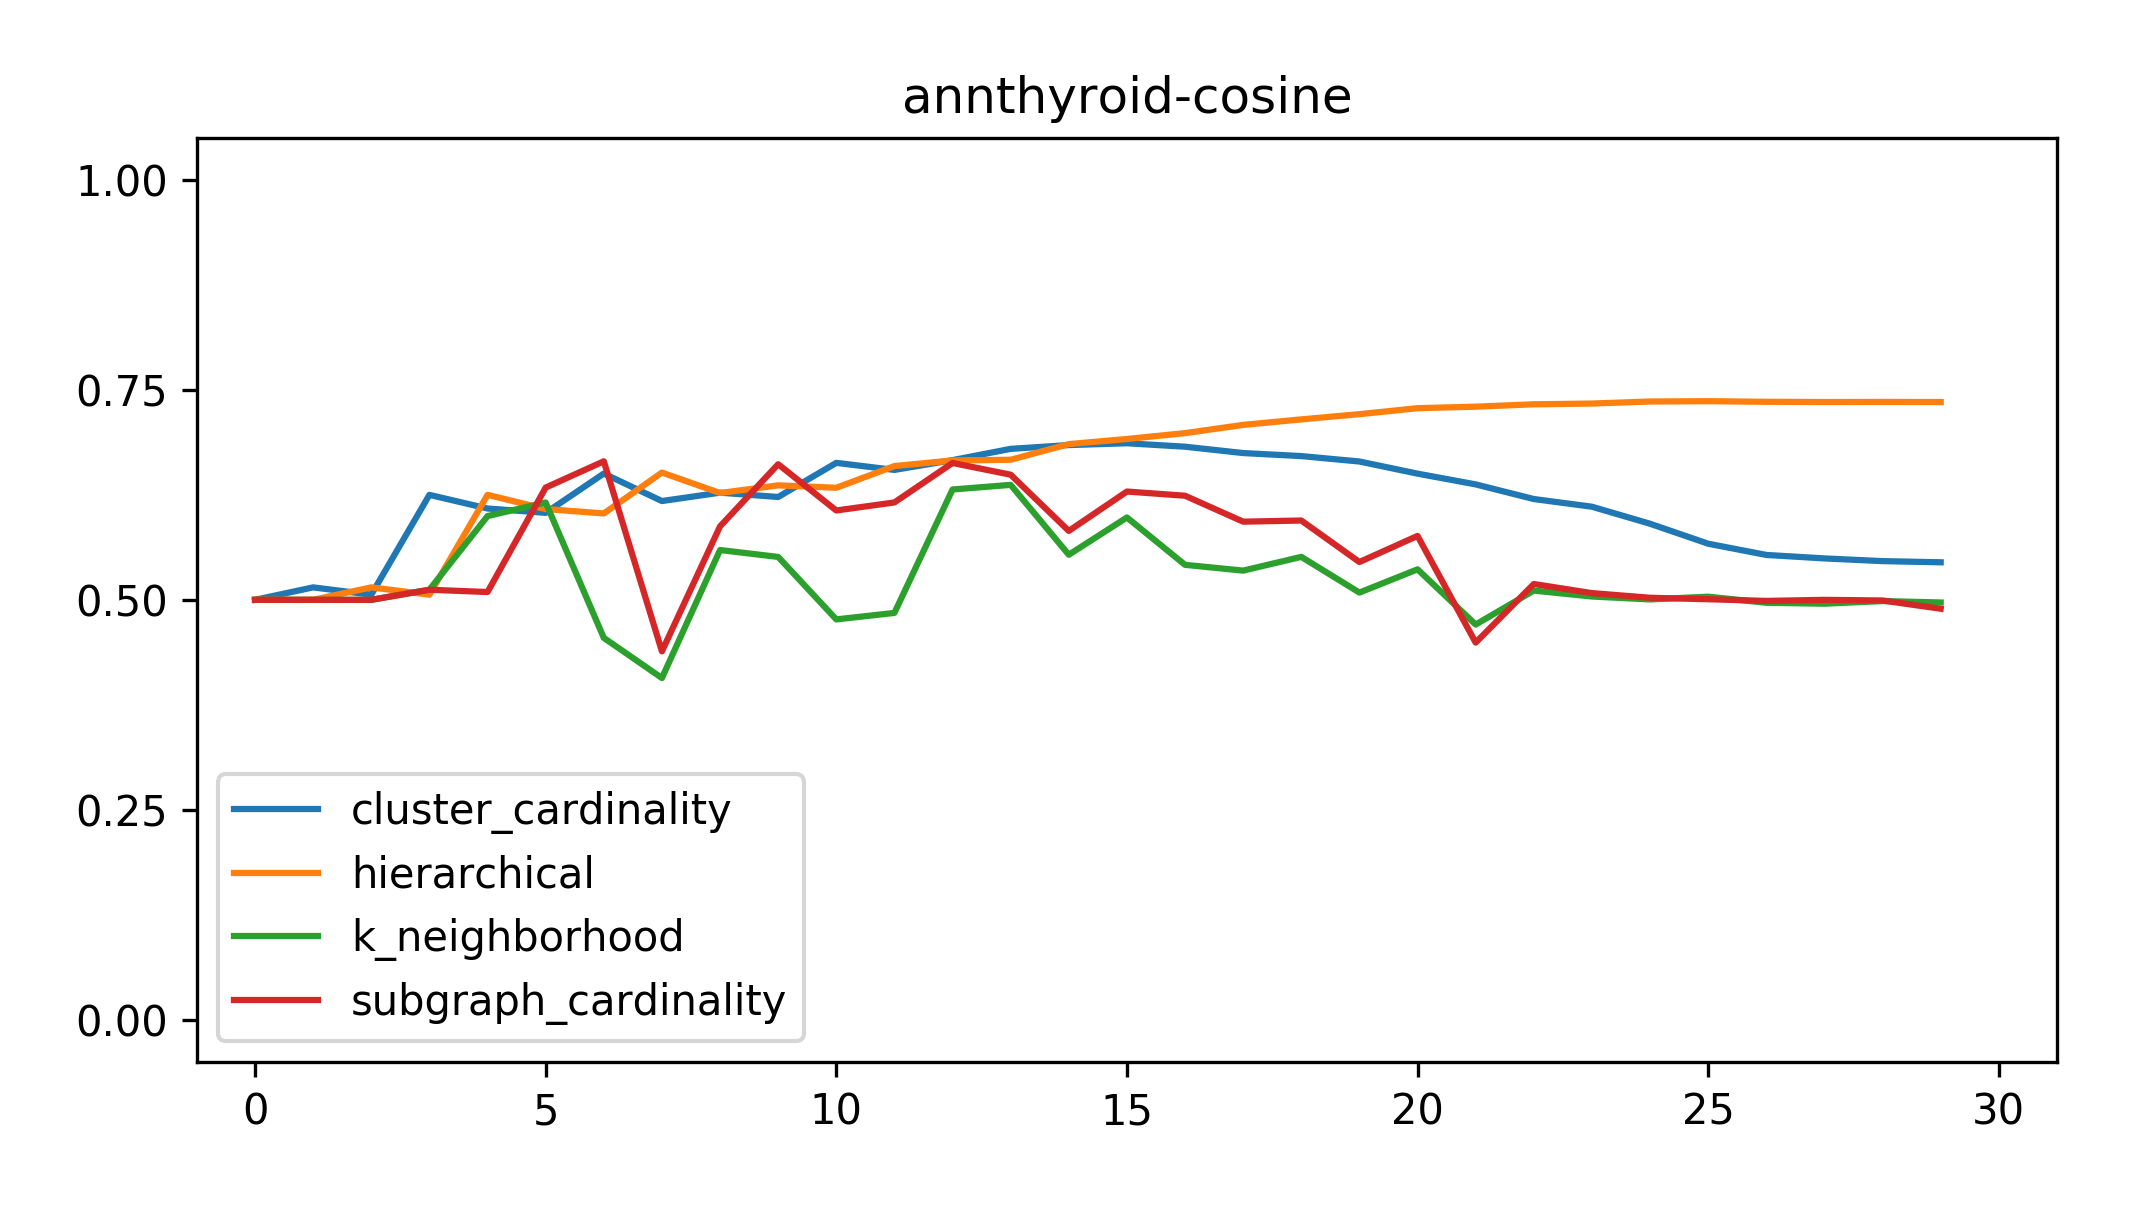
\includegraphics[width=2.2in]{kdd/static/auc_vs_depth/annthyroid-cosine.png}
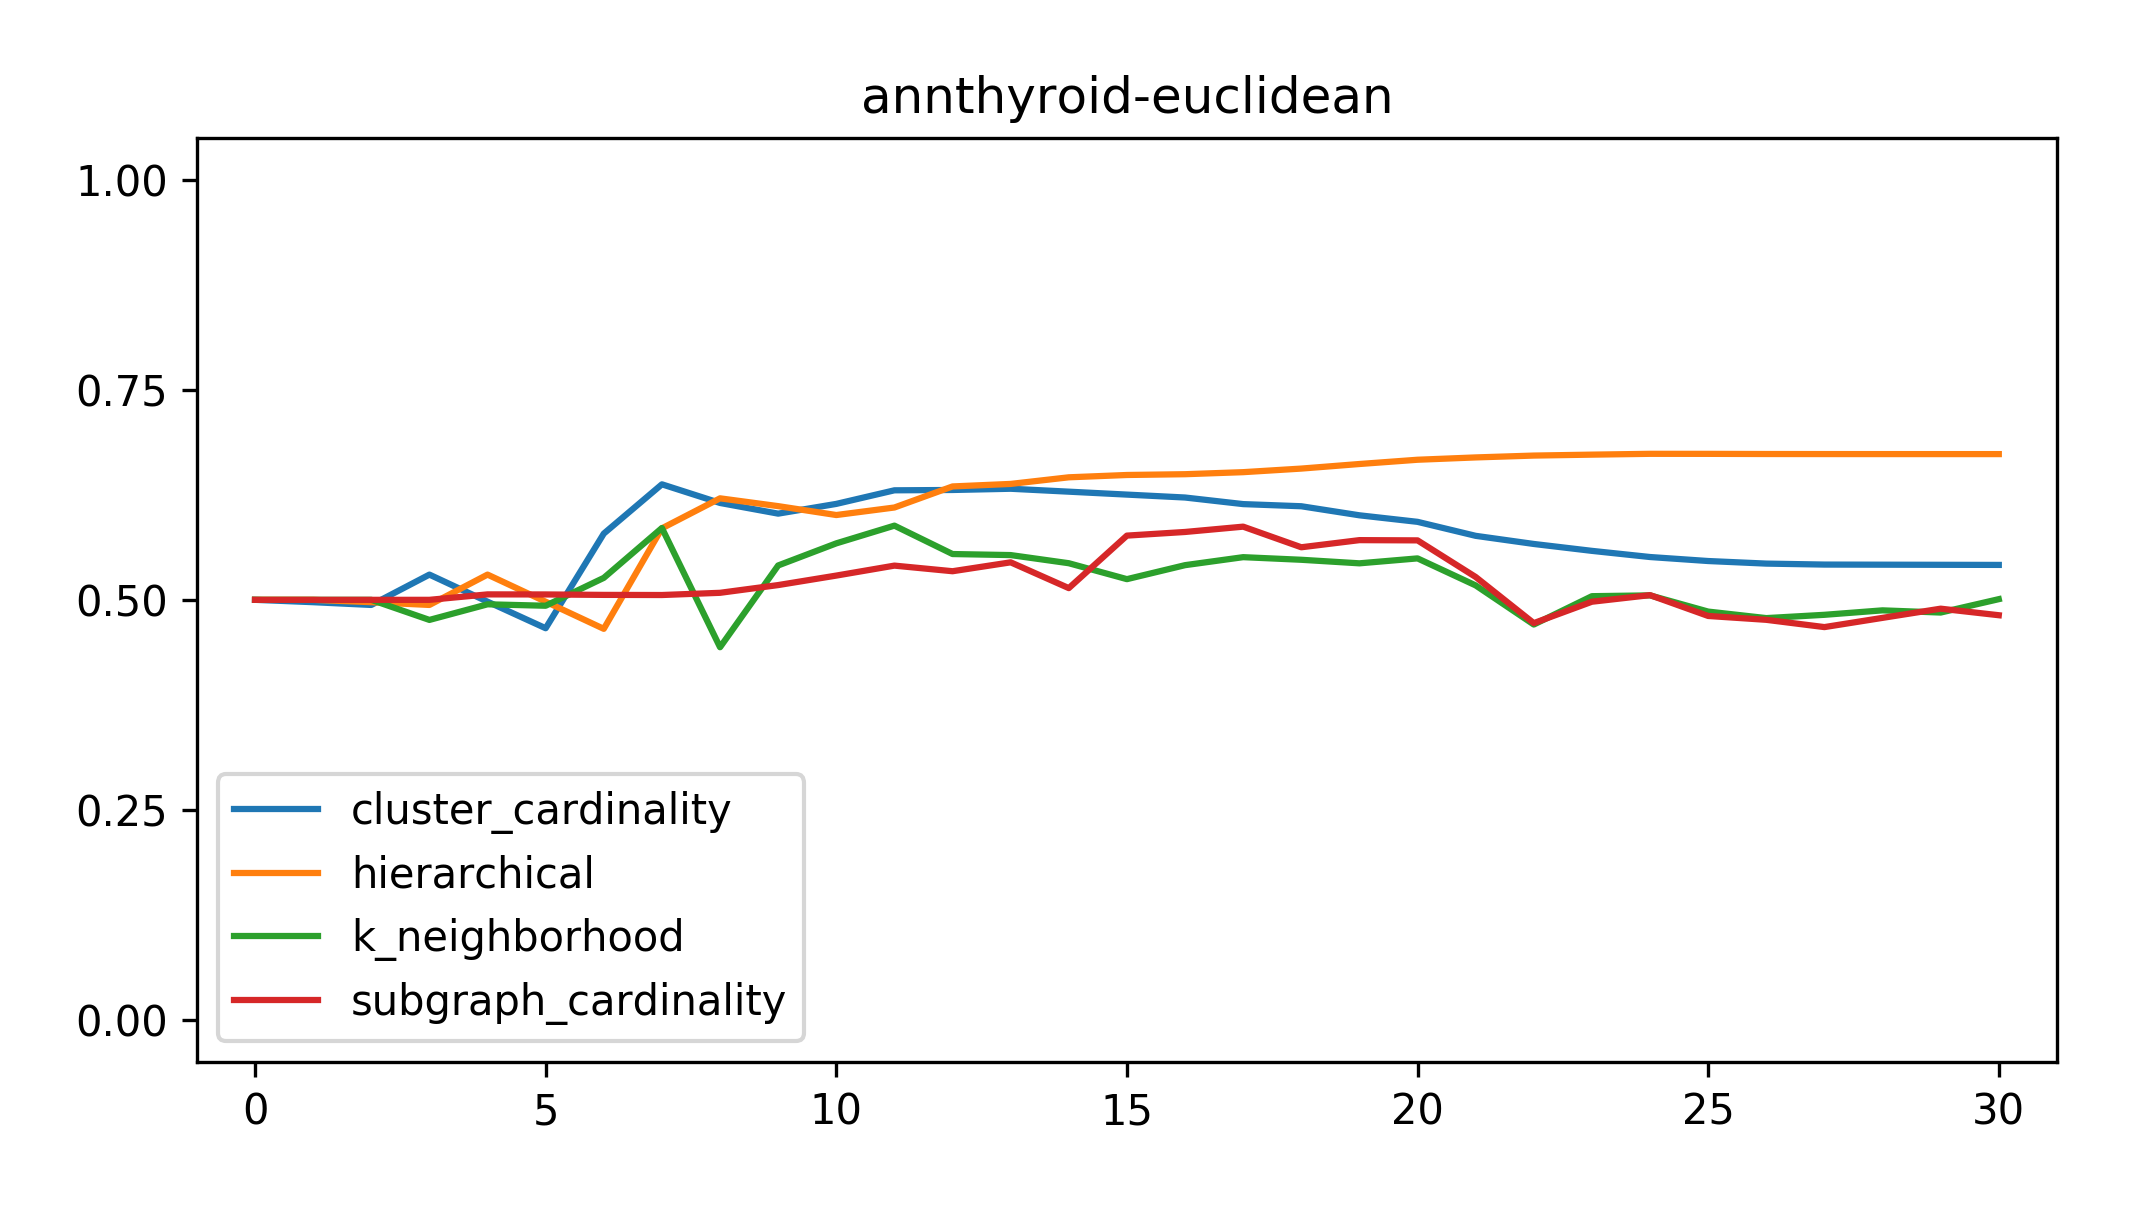
\includegraphics[width=2.2in]{kdd/static/auc_vs_depth/annthyroid-euclidean.png}
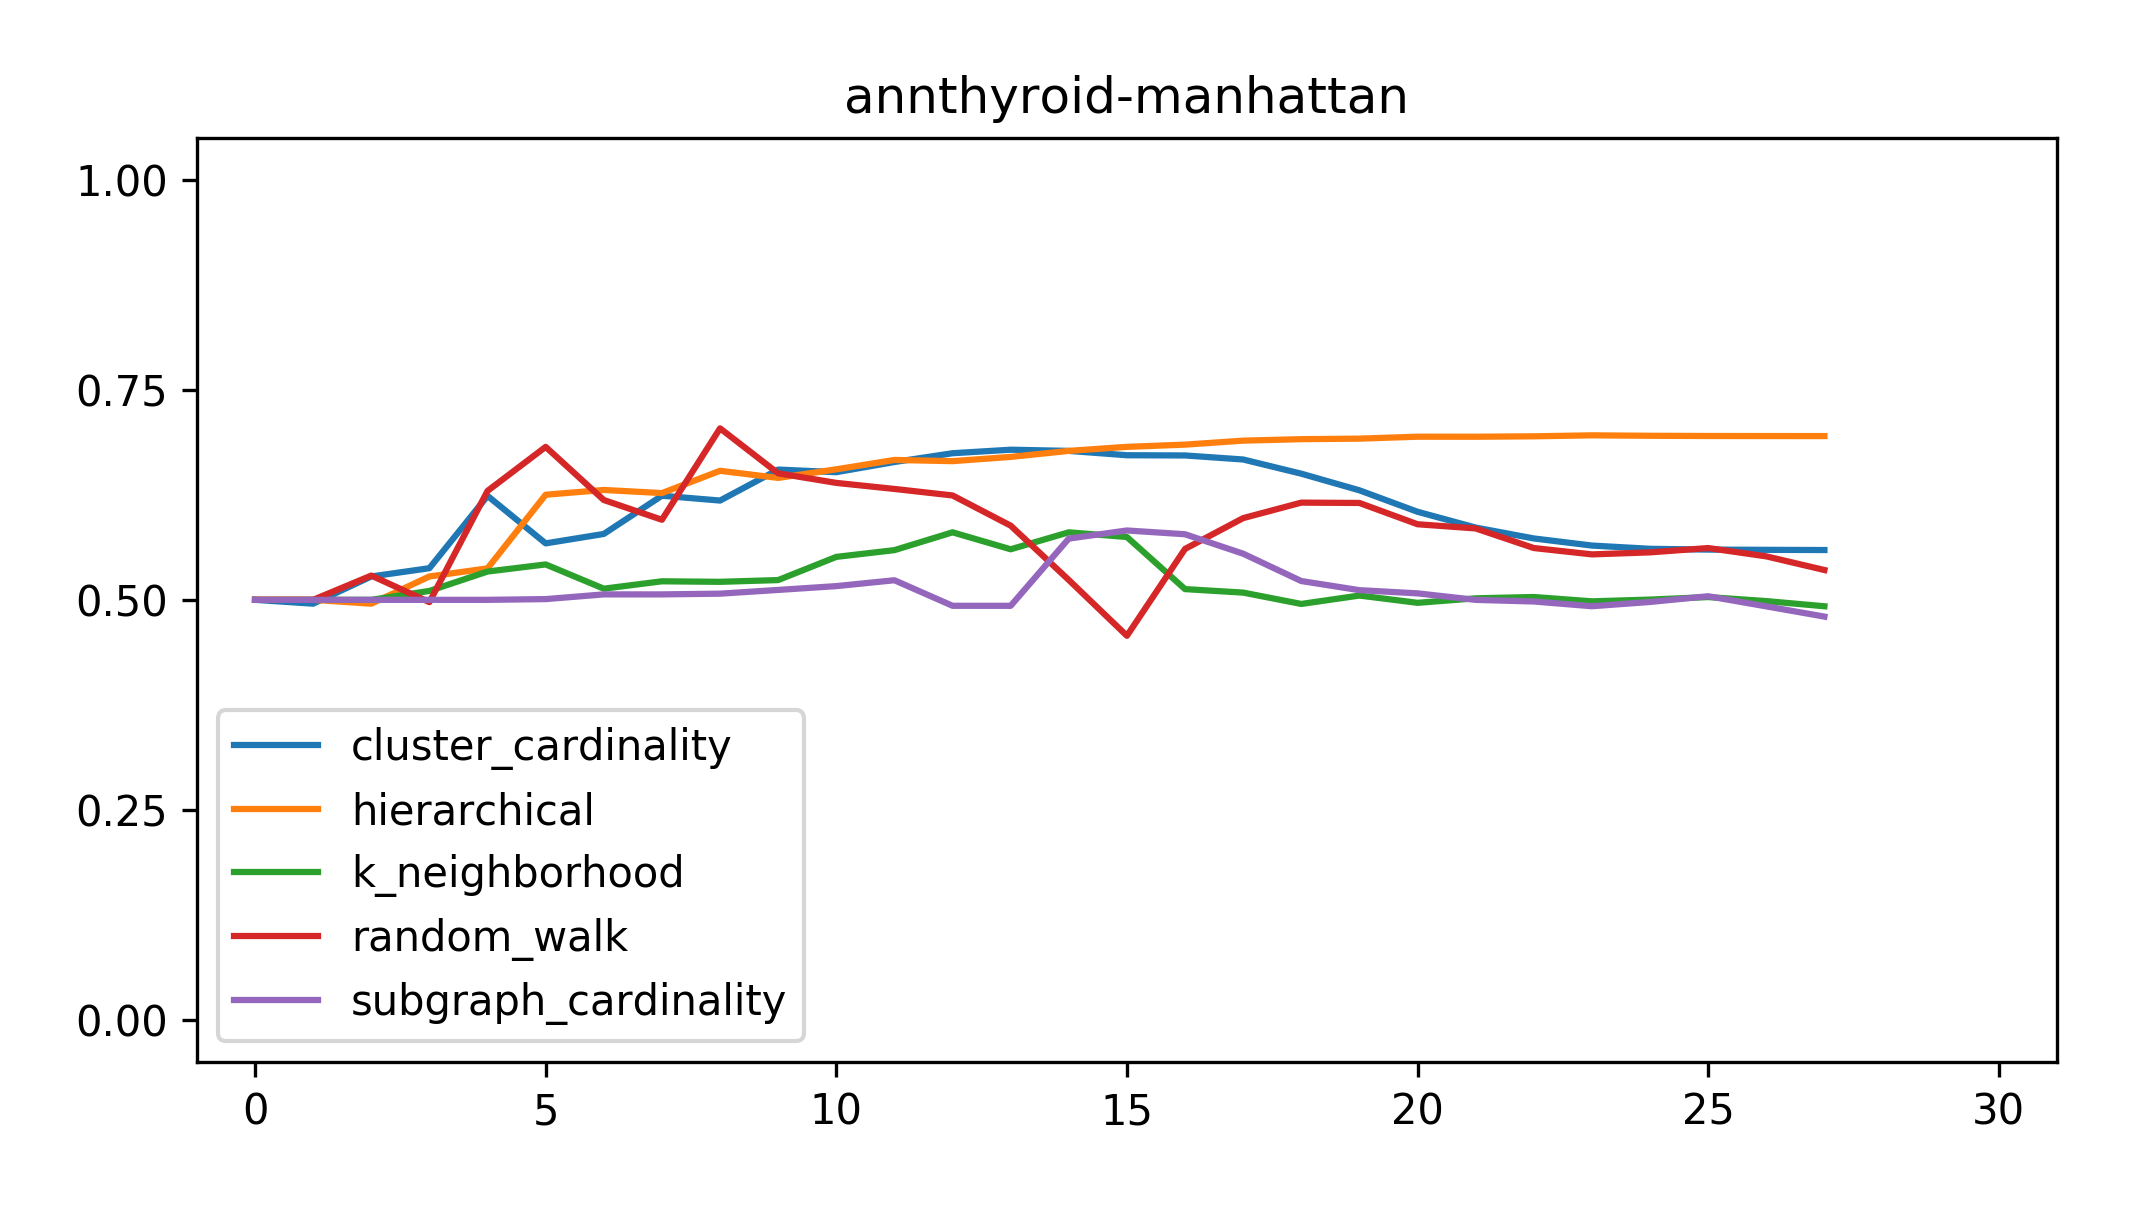
\includegraphics[width=2.2in]{kdd/static/auc_vs_depth/annthyroid-manhattan.png}

% Arrhythmia
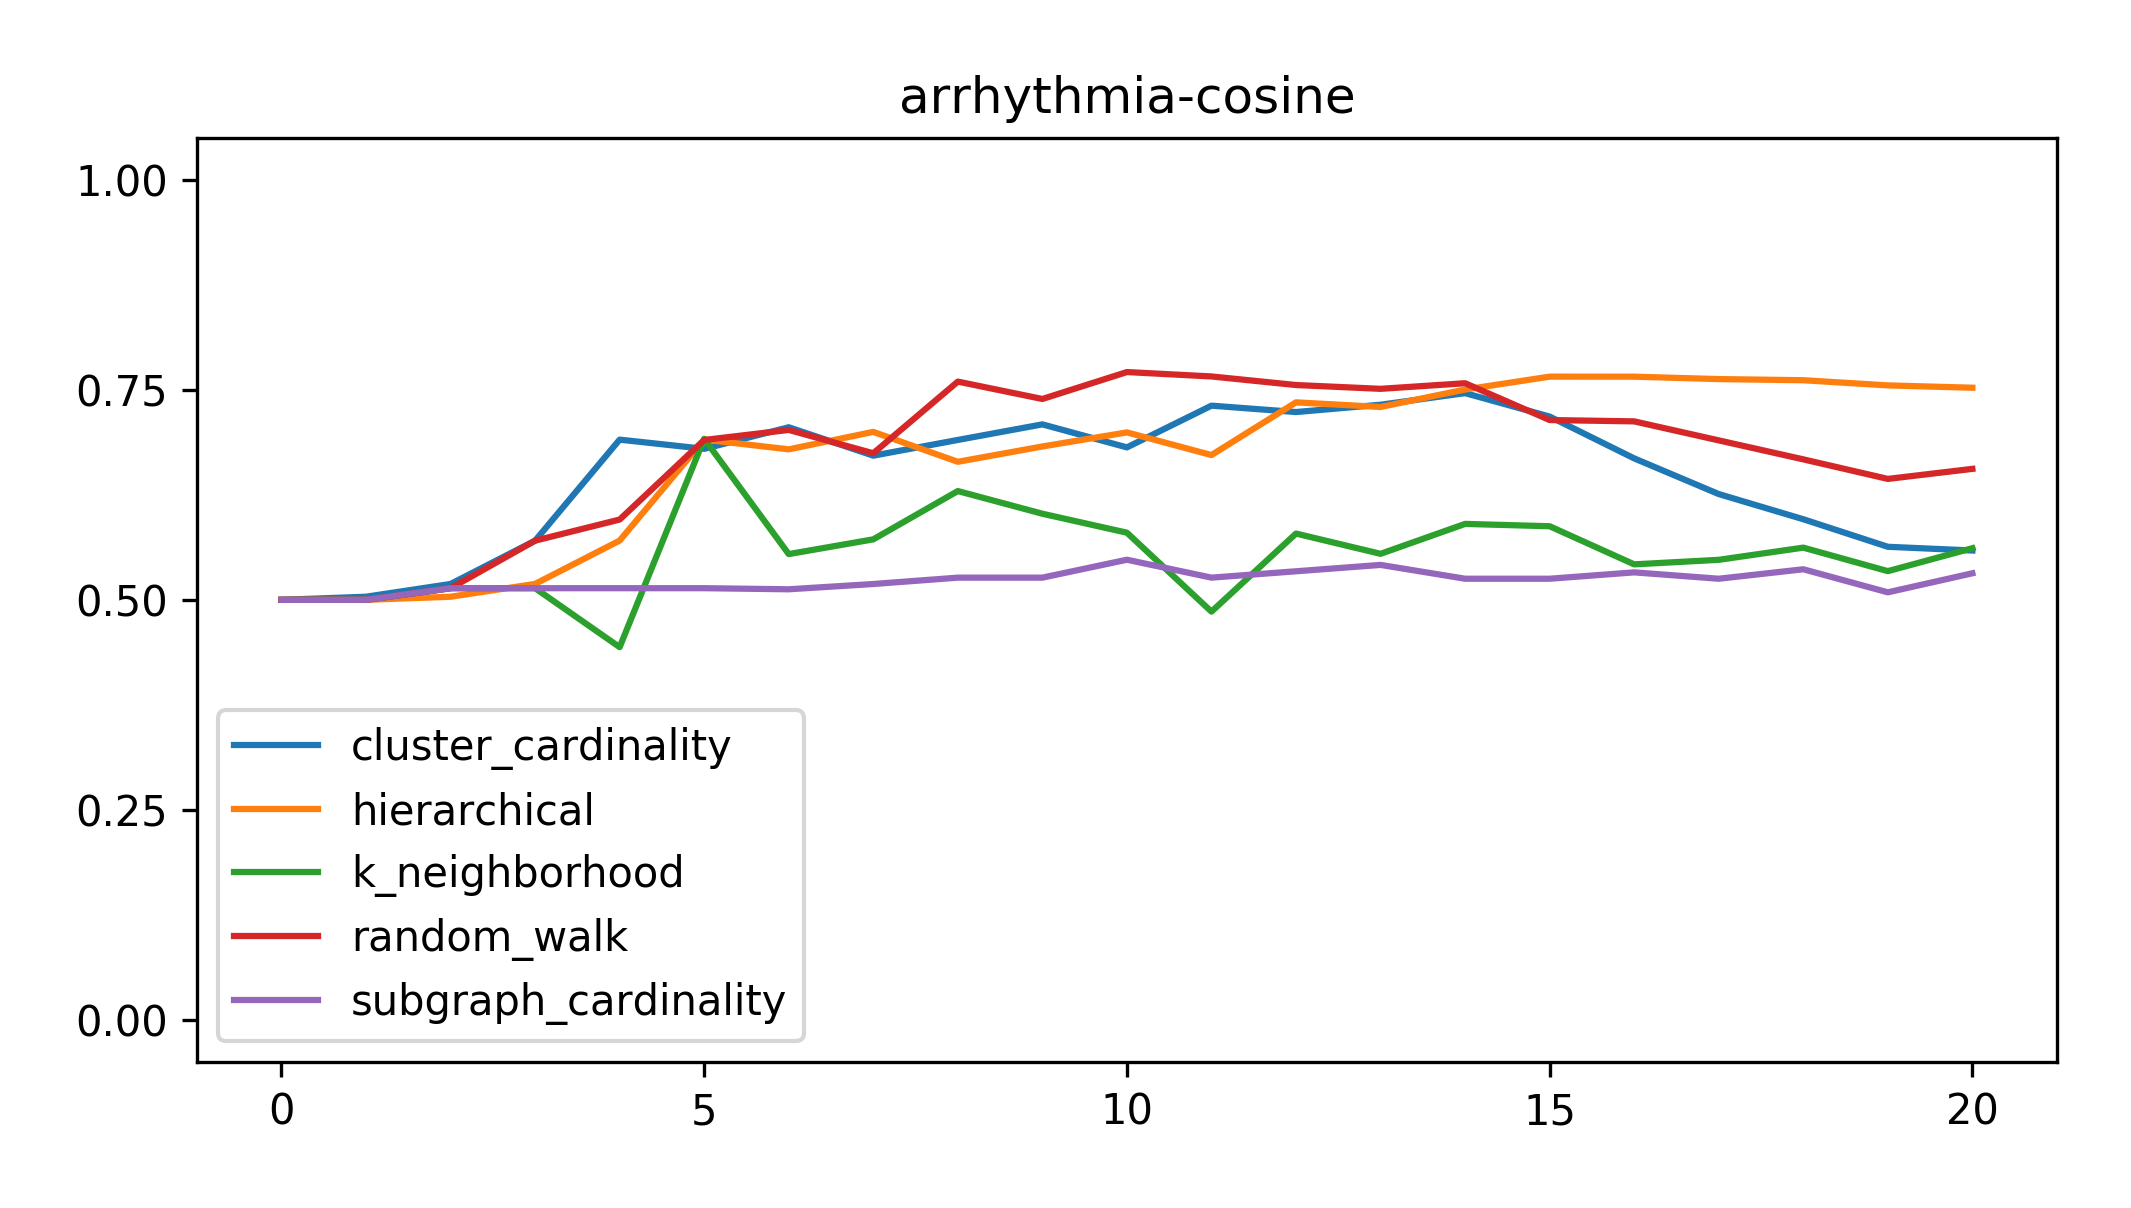
\includegraphics[width=2.2in]{kdd/static/auc_vs_depth/arrhythmia-cosine.png}
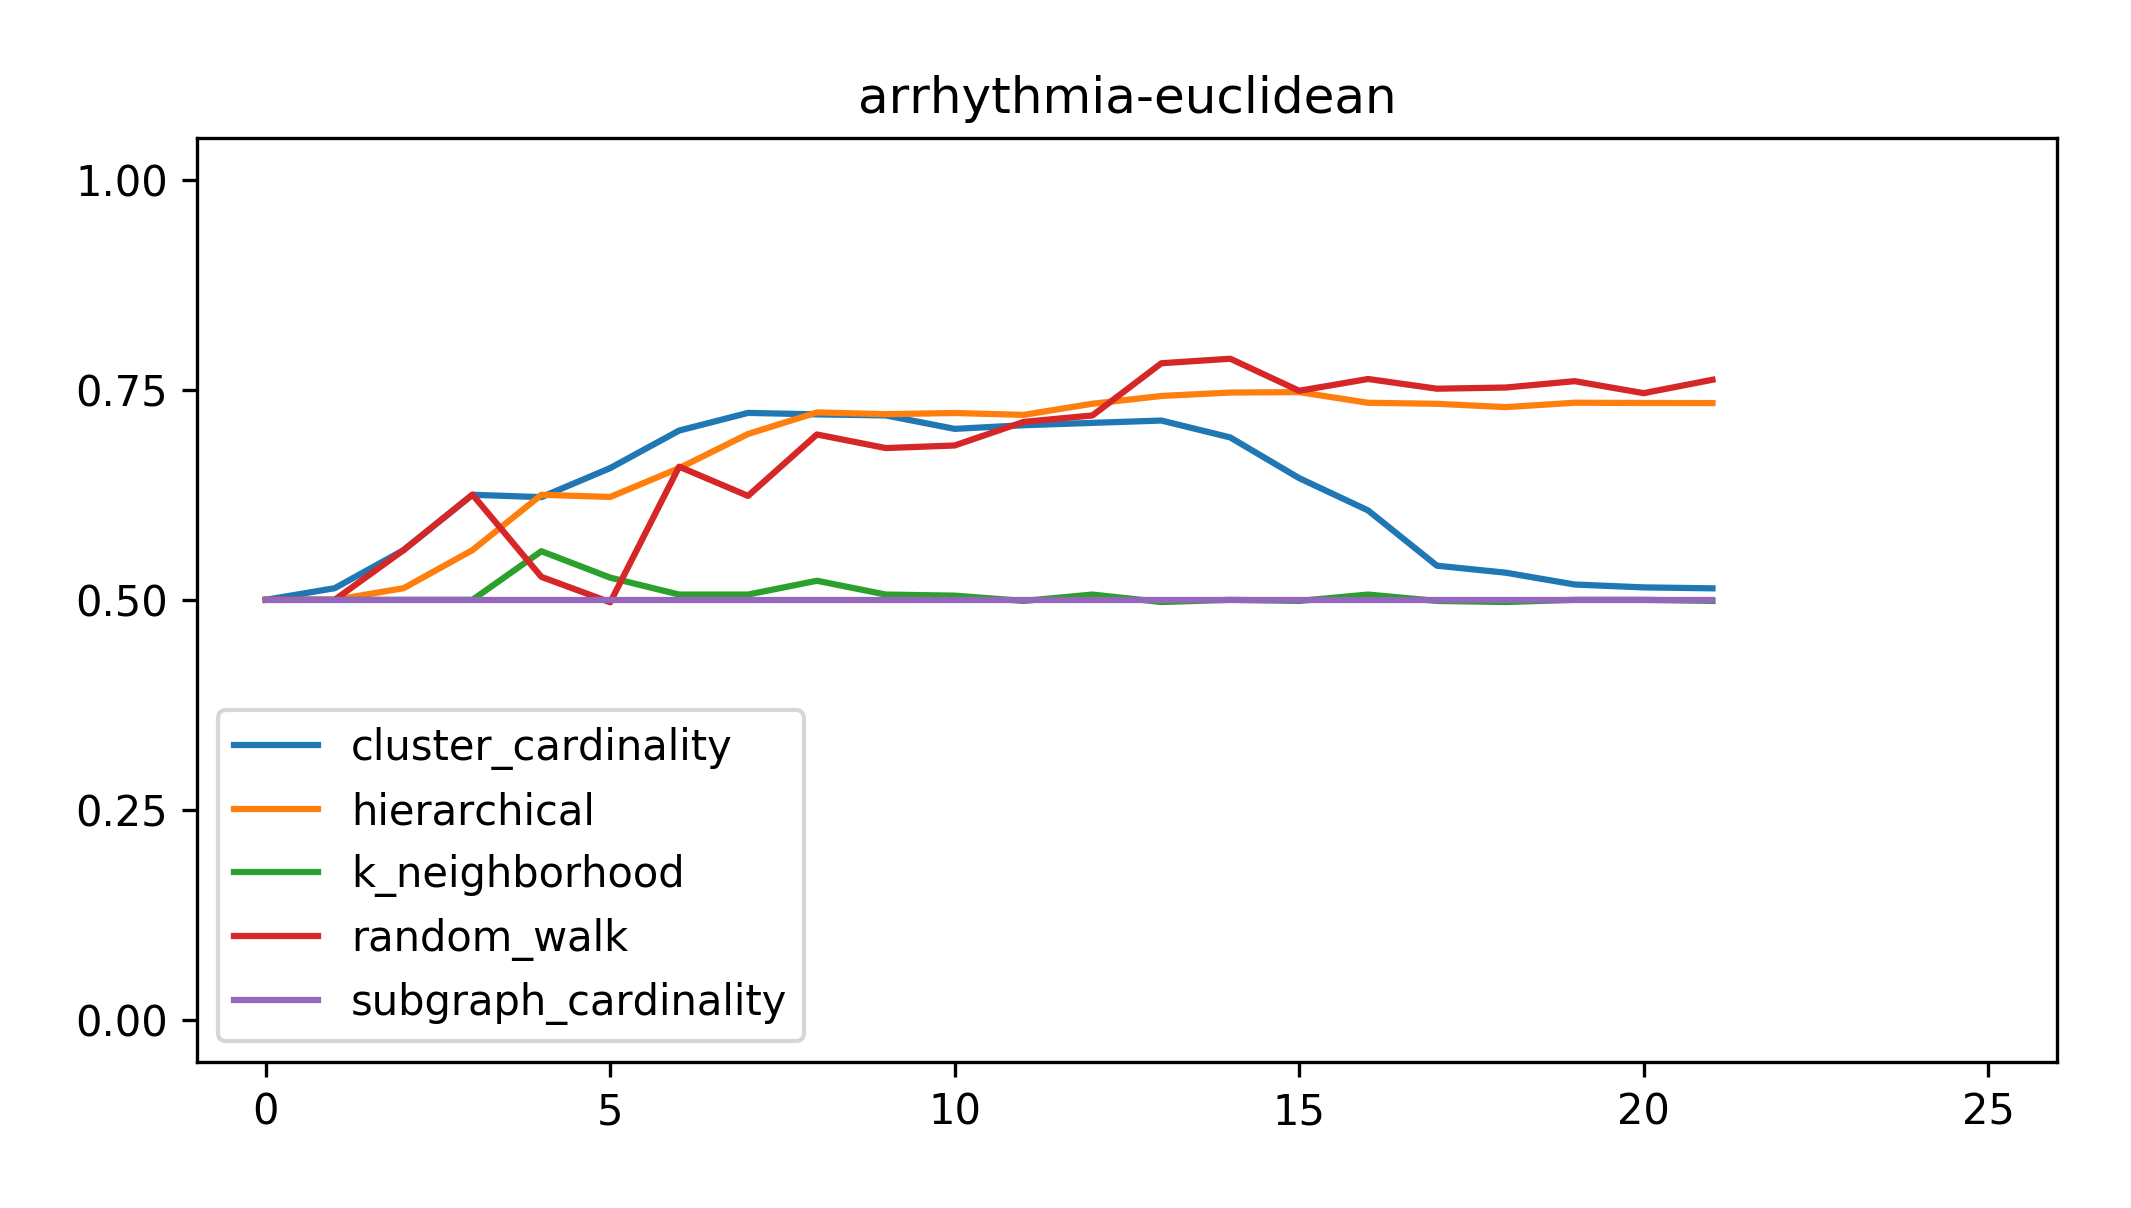
\includegraphics[width=2.2in]{kdd/static/auc_vs_depth/arrhythmia-euclidean.png}
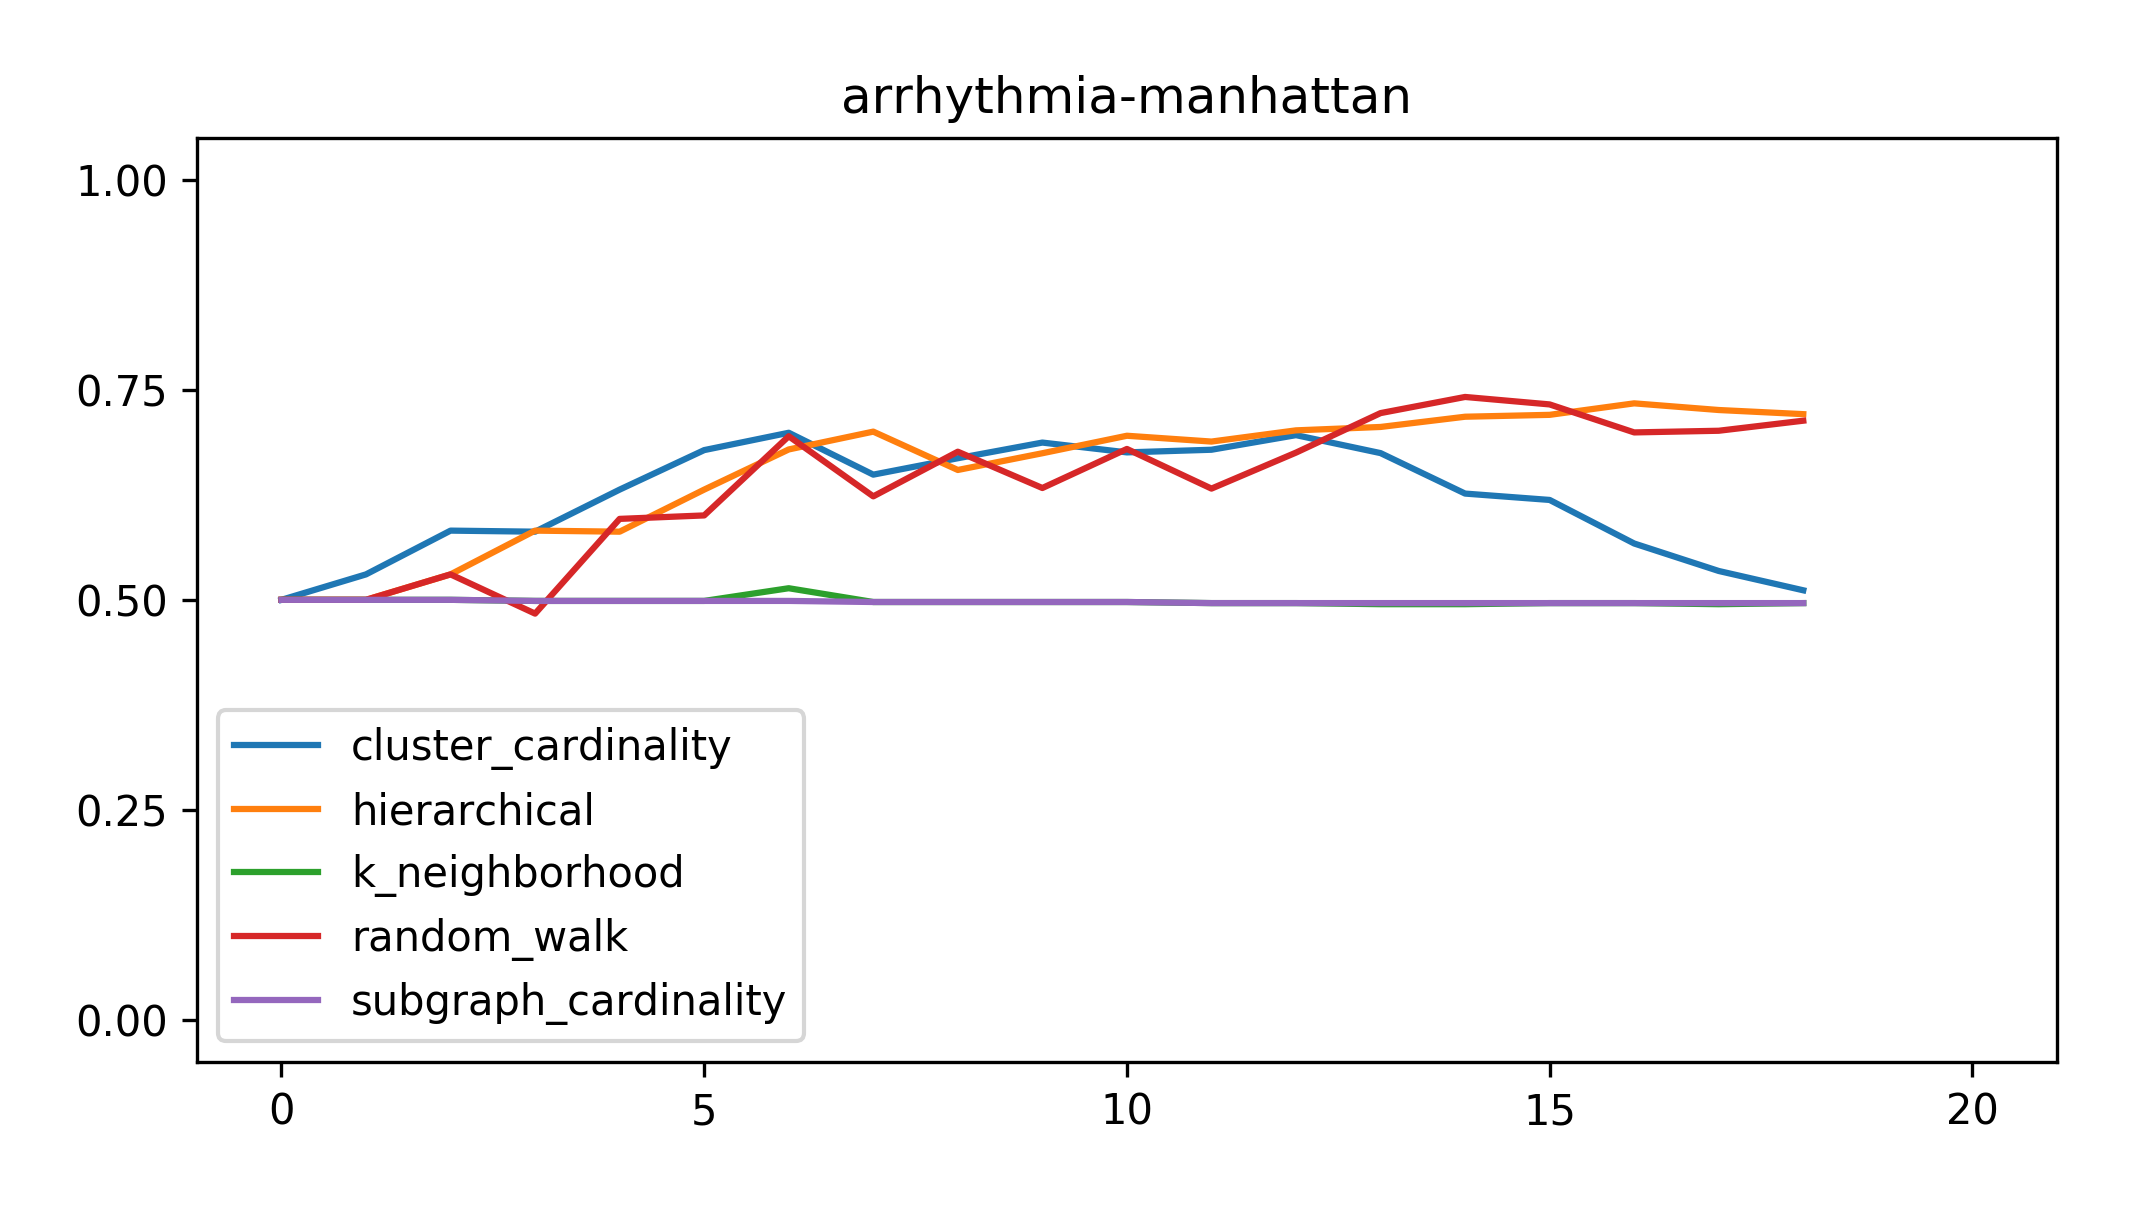
\includegraphics[width=2.2in]{kdd/static/auc_vs_depth/arrhythmia-manhattan.png}

% BreastW
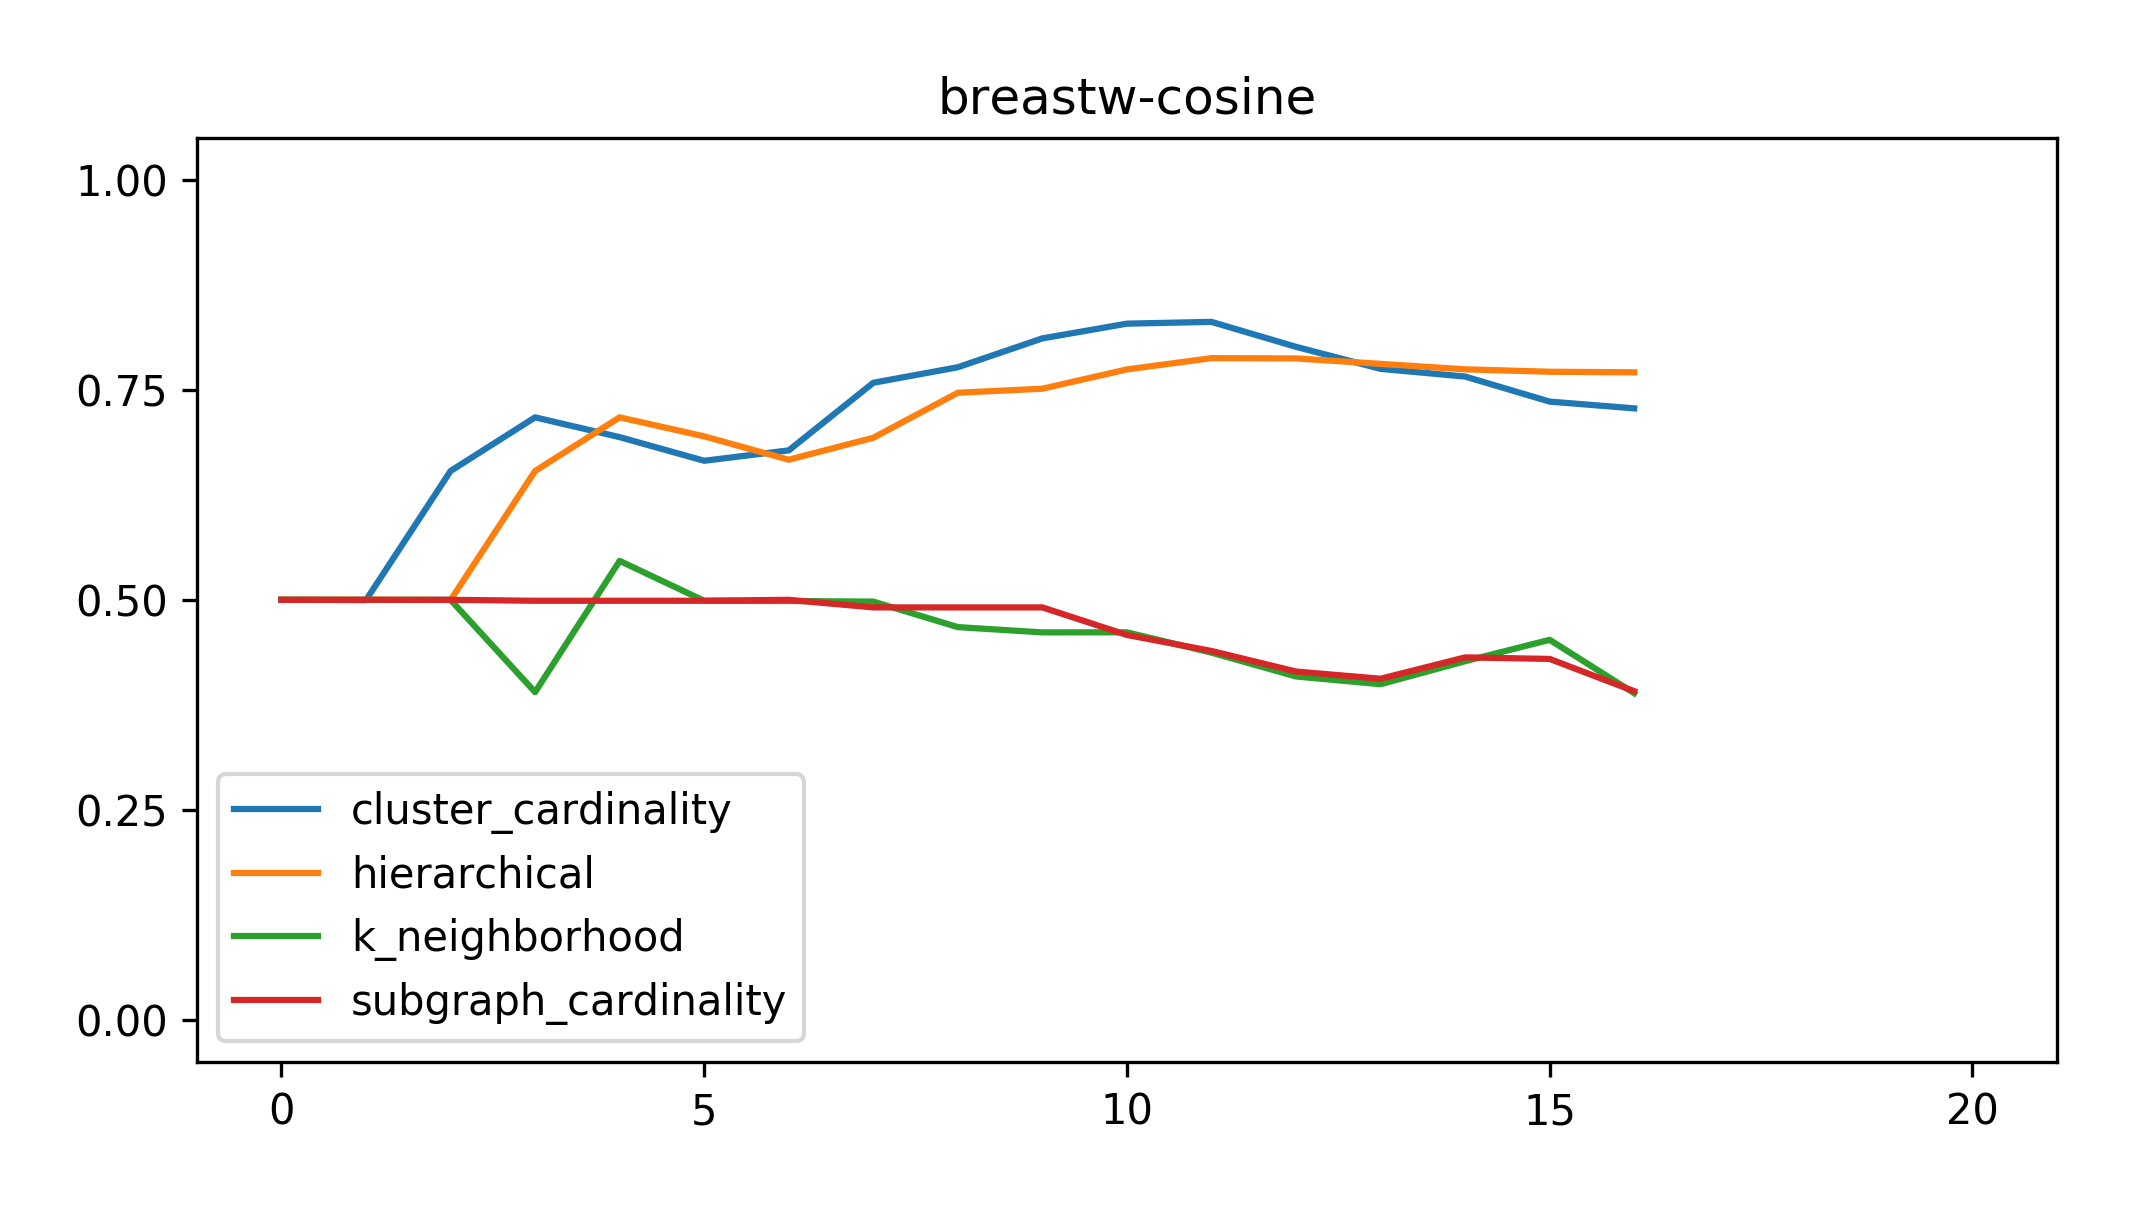
\includegraphics[width=2.2in]{kdd/static/auc_vs_depth/breastw-cosine.png}
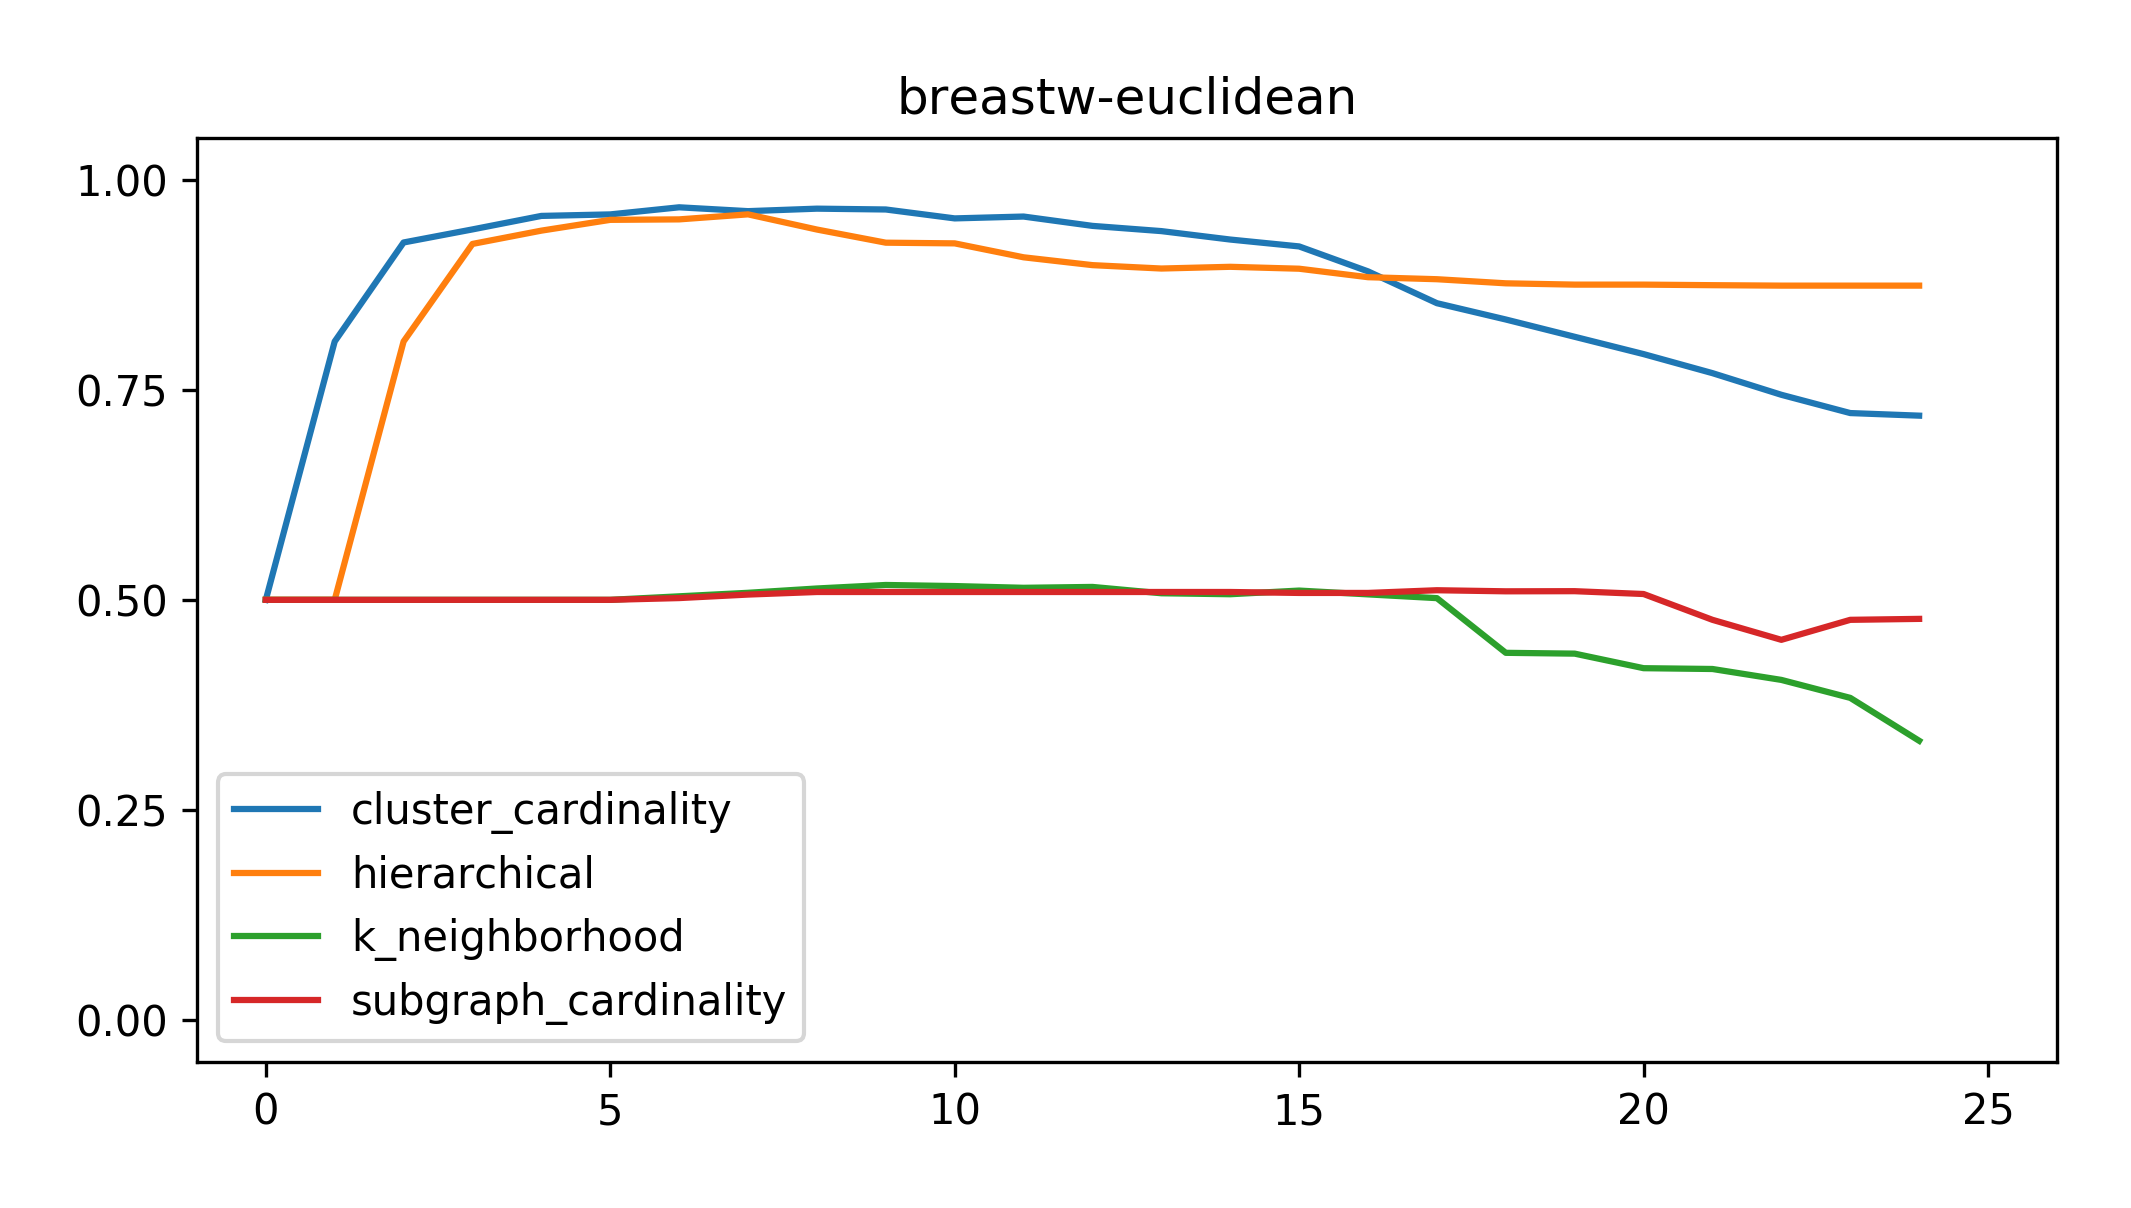
\includegraphics[width=2.2in]{kdd/static/auc_vs_depth/breastw-euclidean.png}
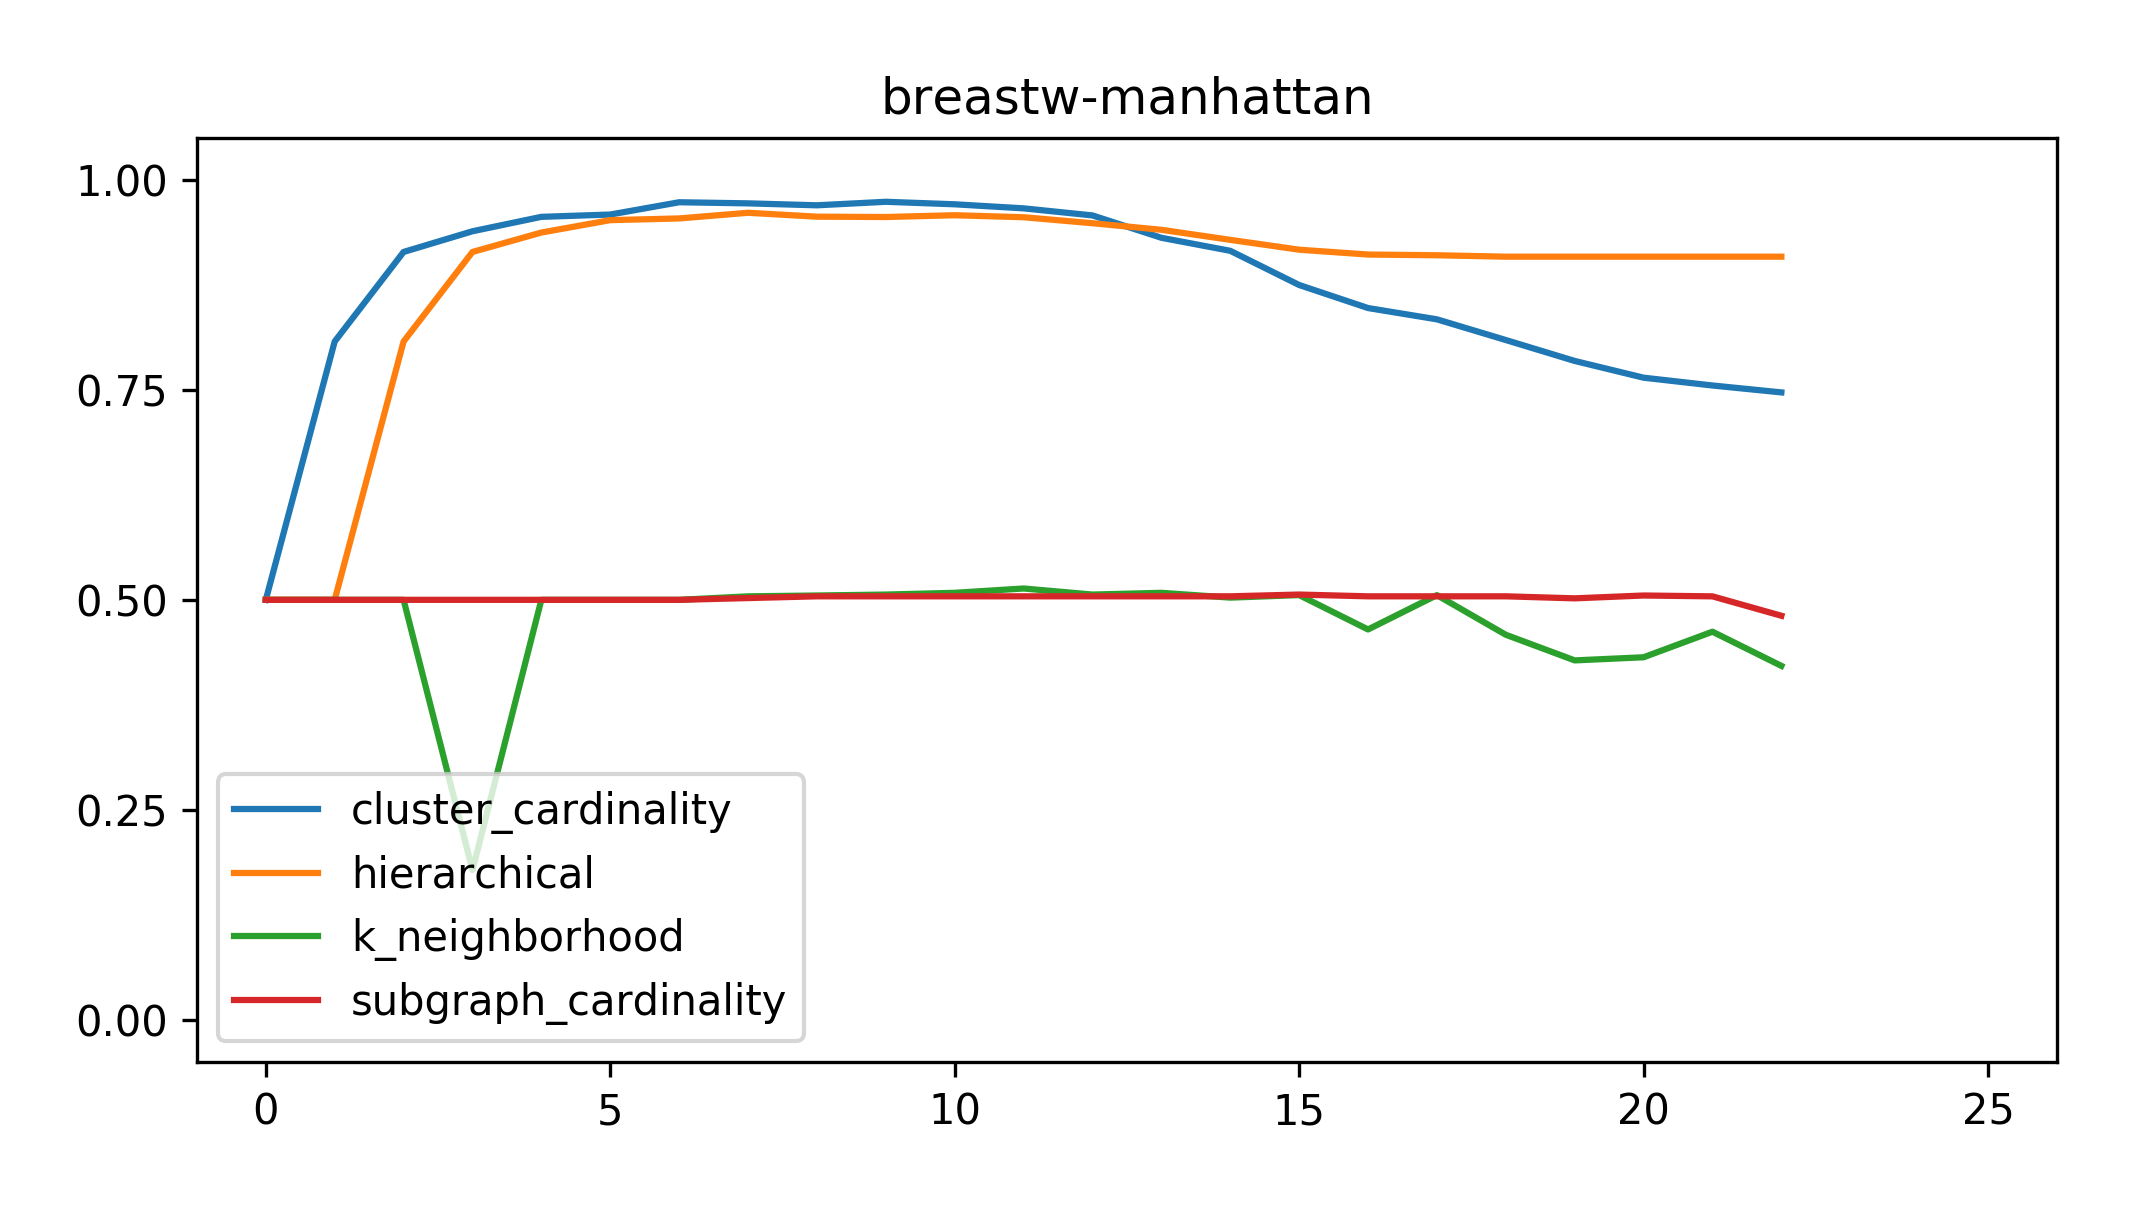
\includegraphics[width=2.2in]{kdd/static/auc_vs_depth/breastw-manhattan.png}

% Cardio
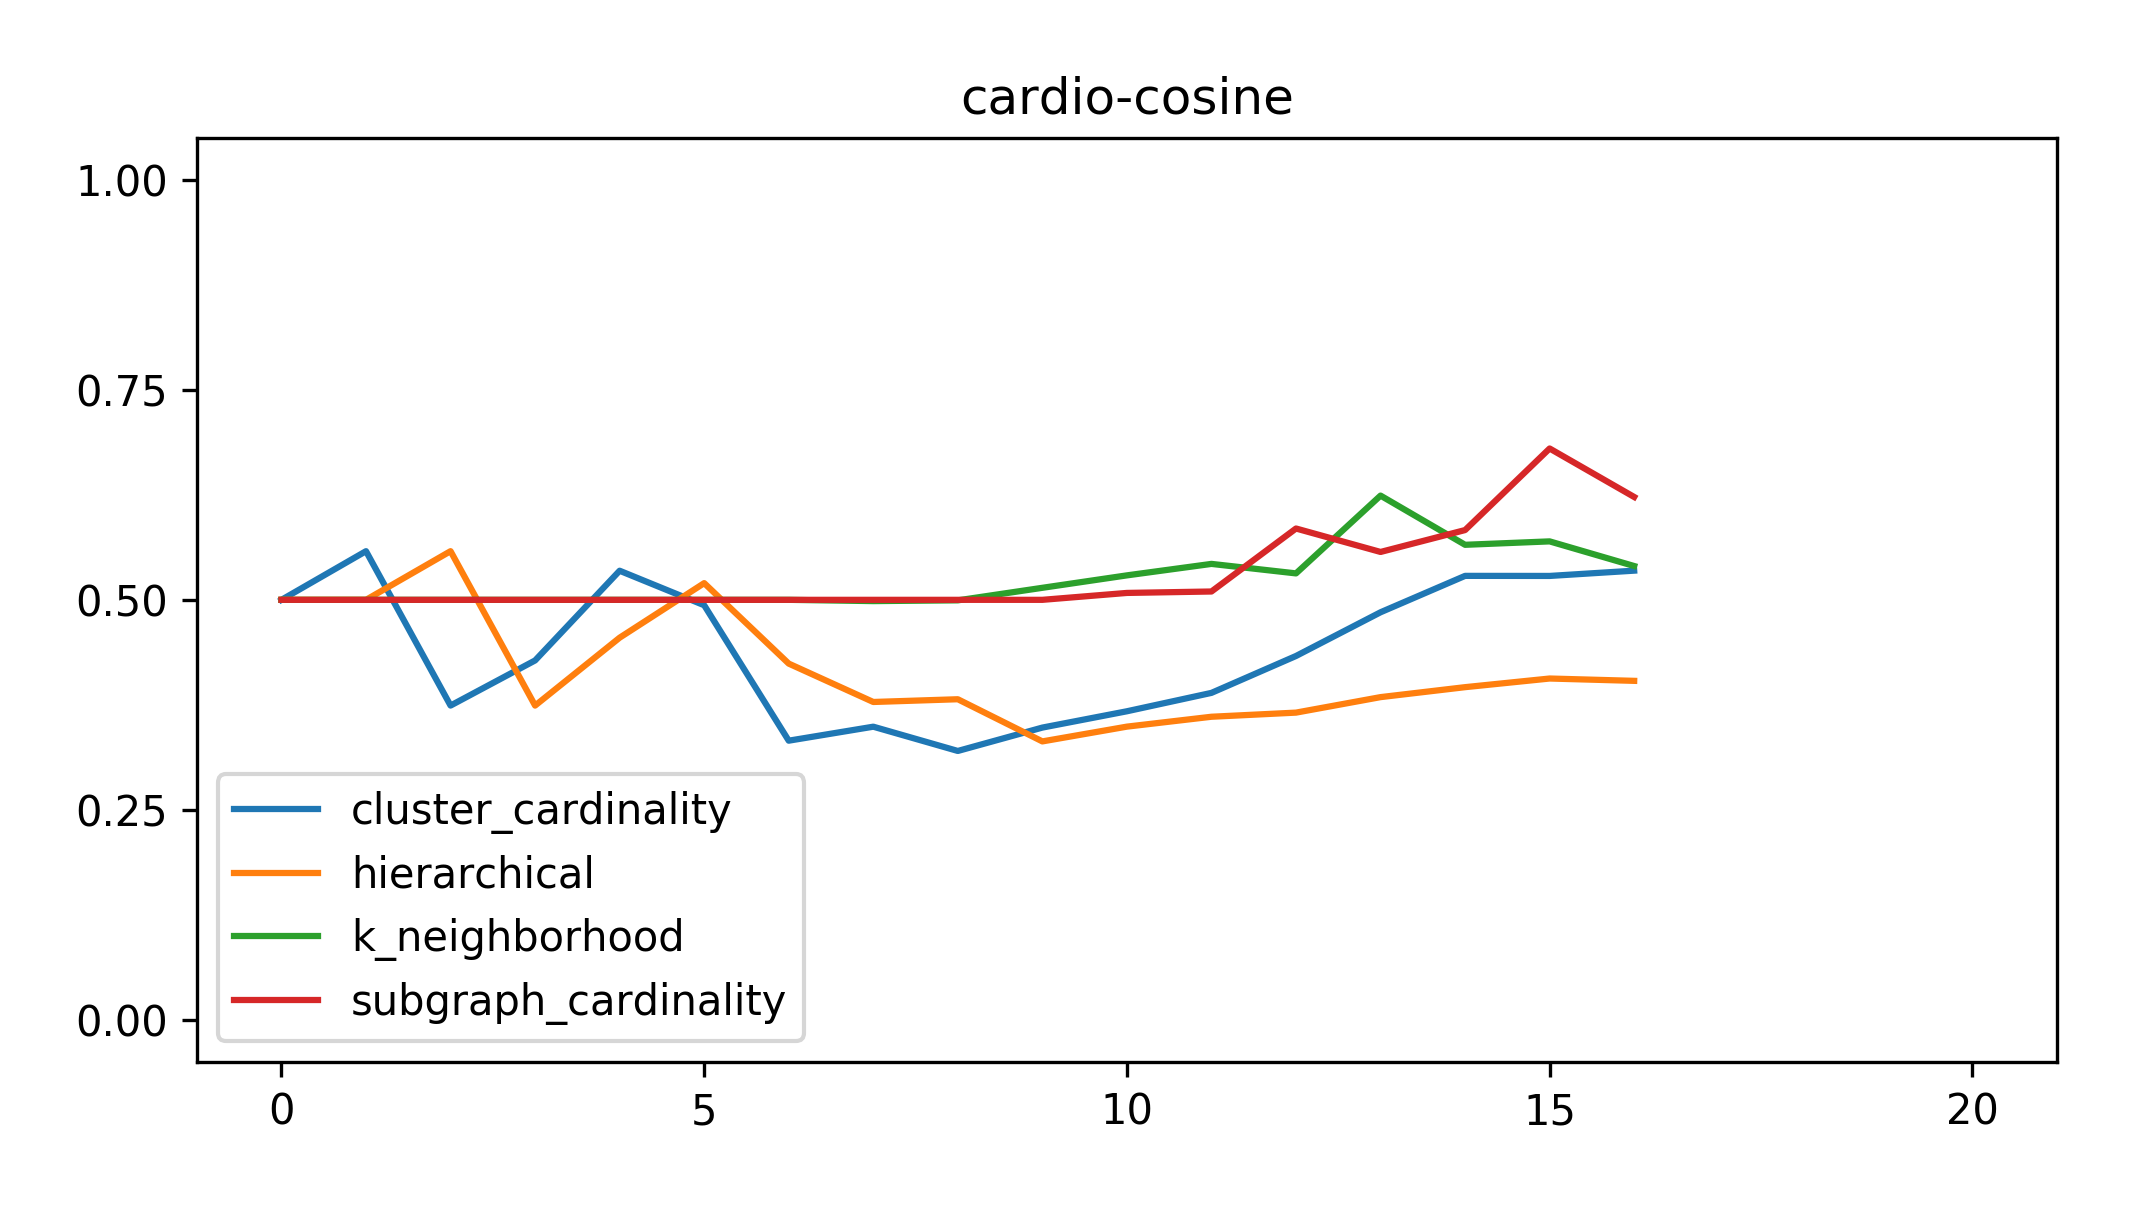
\includegraphics[width=2.2in]{kdd/static/auc_vs_depth/cardio-cosine.png}
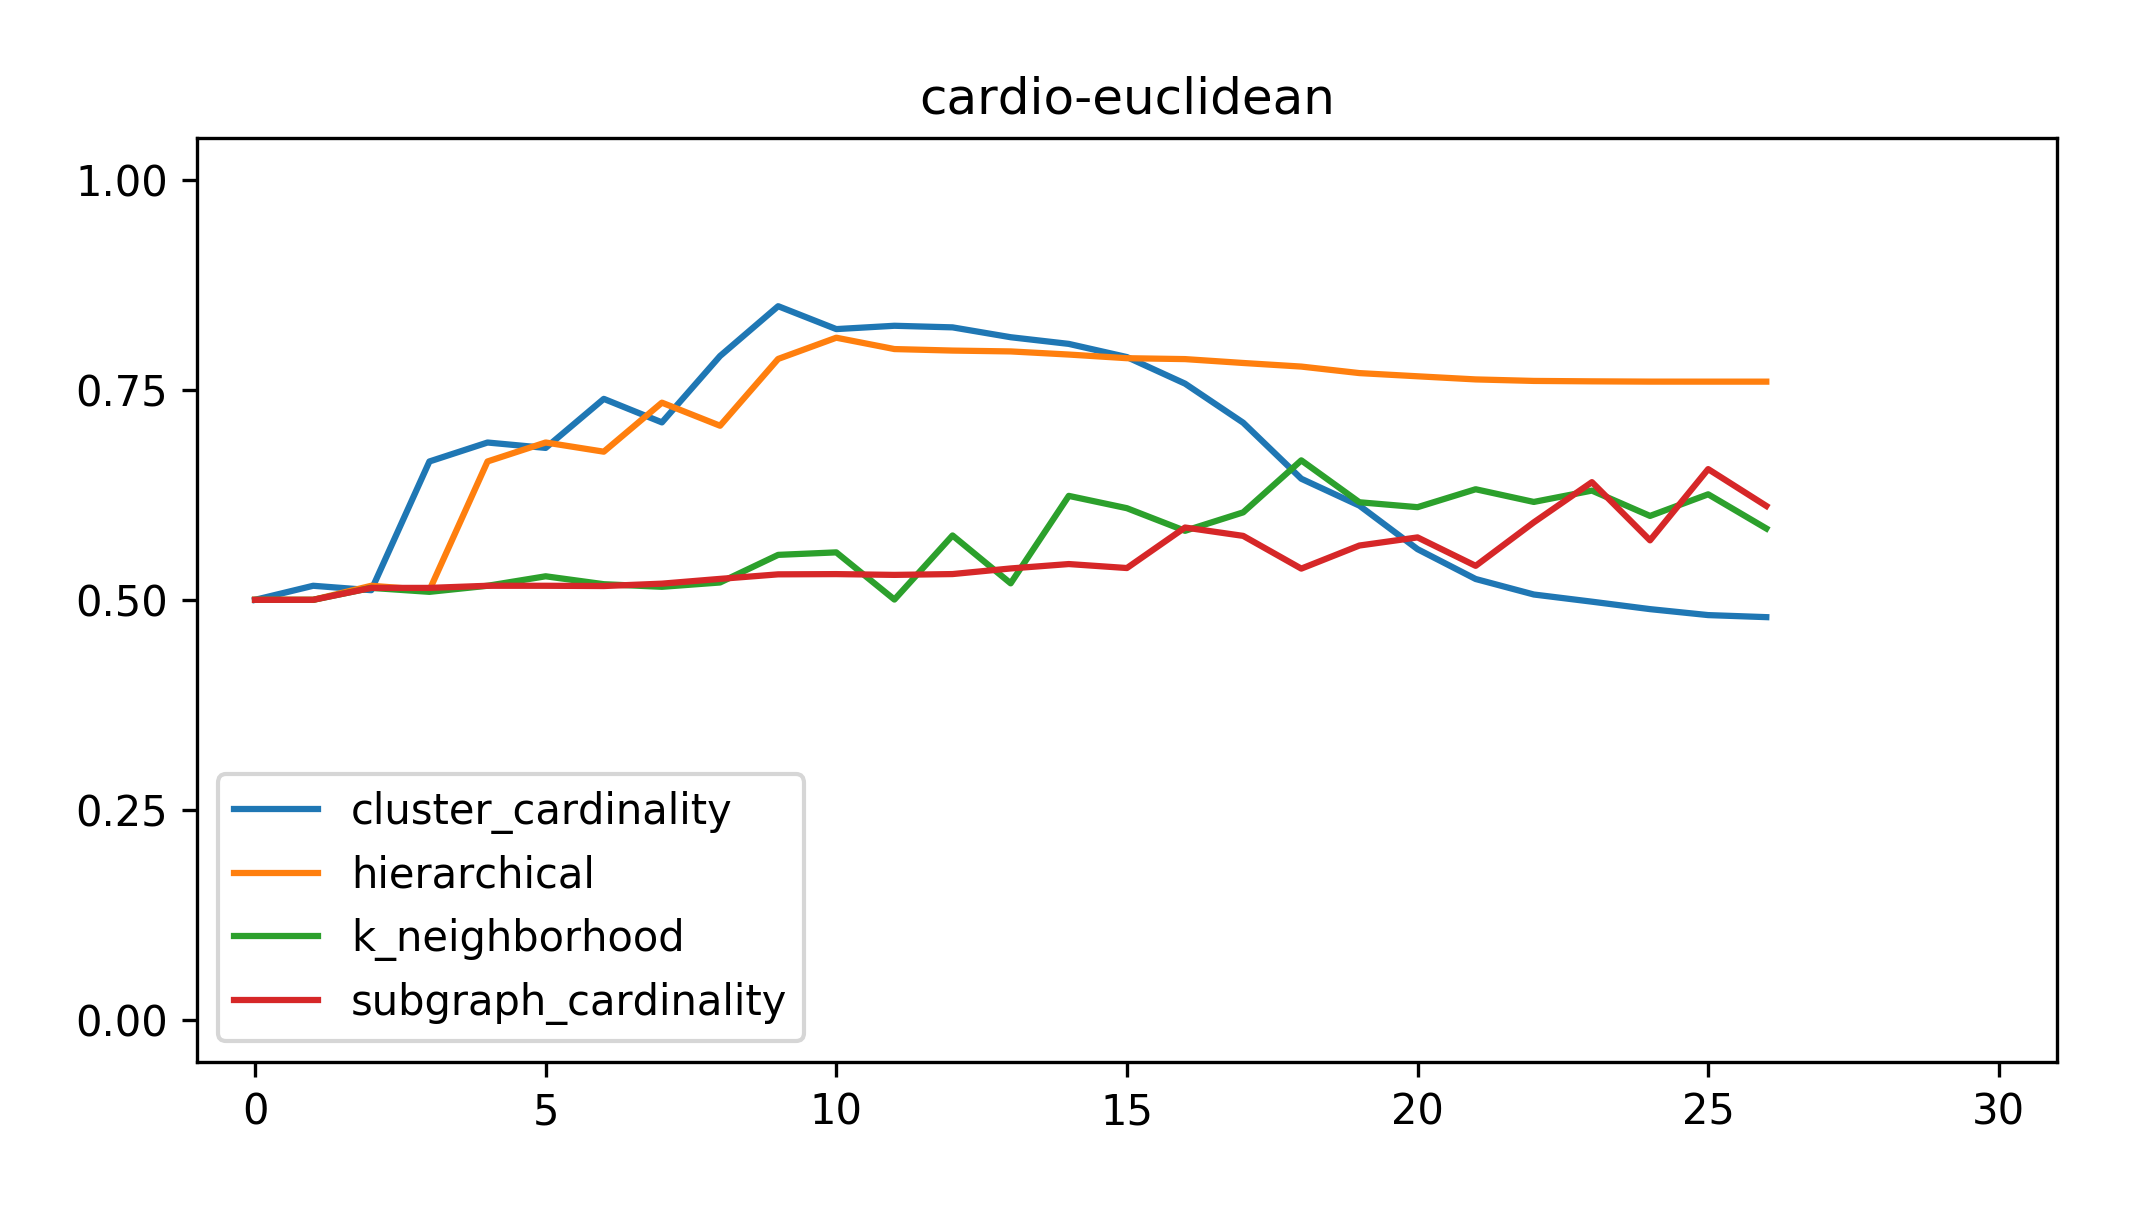
\includegraphics[width=2.2in]{kdd/static/auc_vs_depth/cardio-euclidean.png}
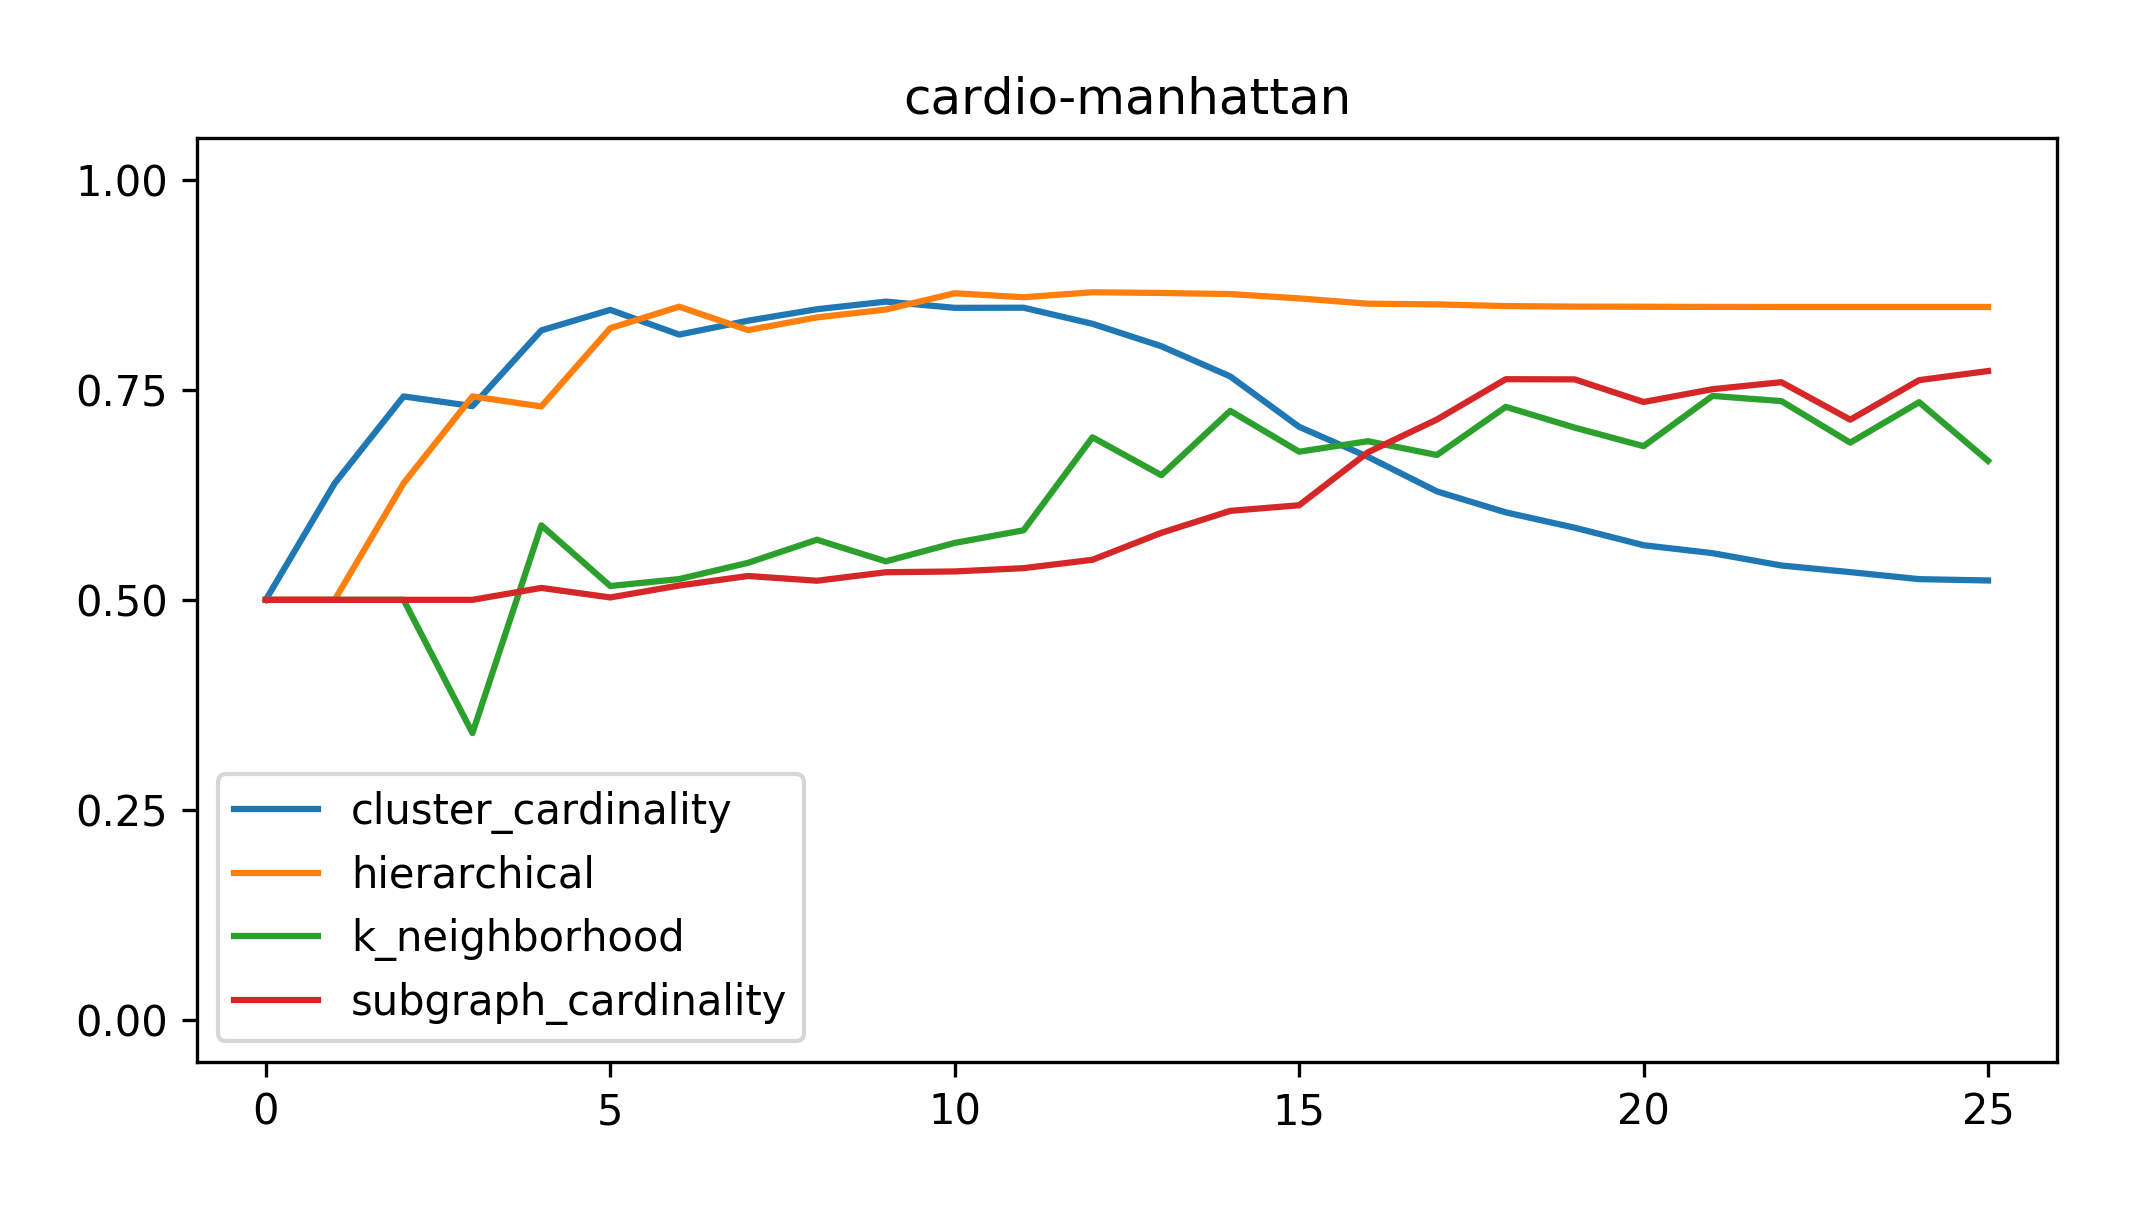
\includegraphics[width=2.2in]{kdd/static/auc_vs_depth/cardio-manhattan.png}

% Glass
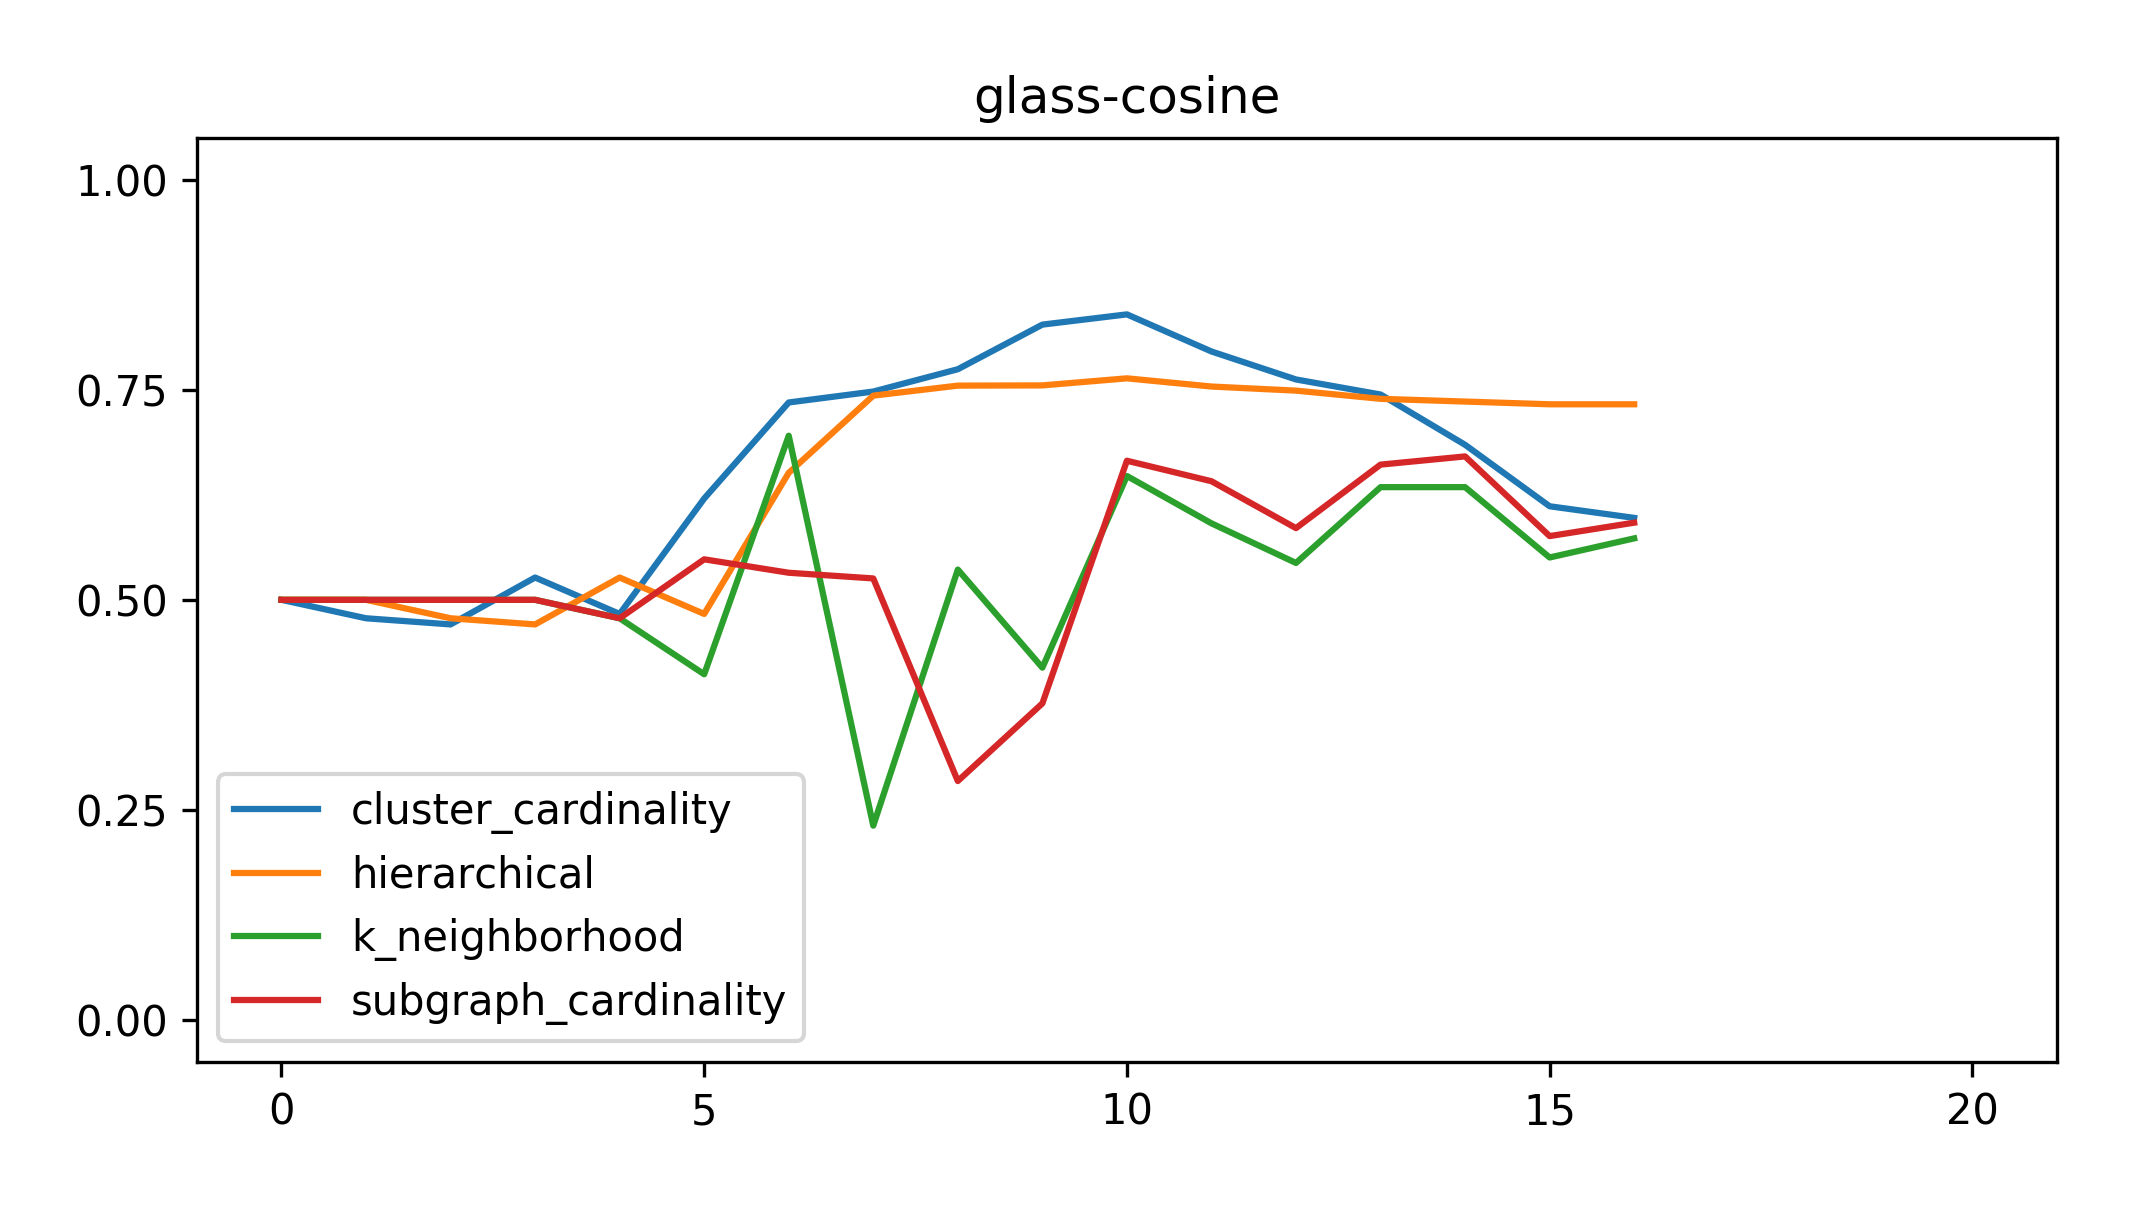
\includegraphics[width=2.2in]{kdd/static/auc_vs_depth/glass-cosine.png}
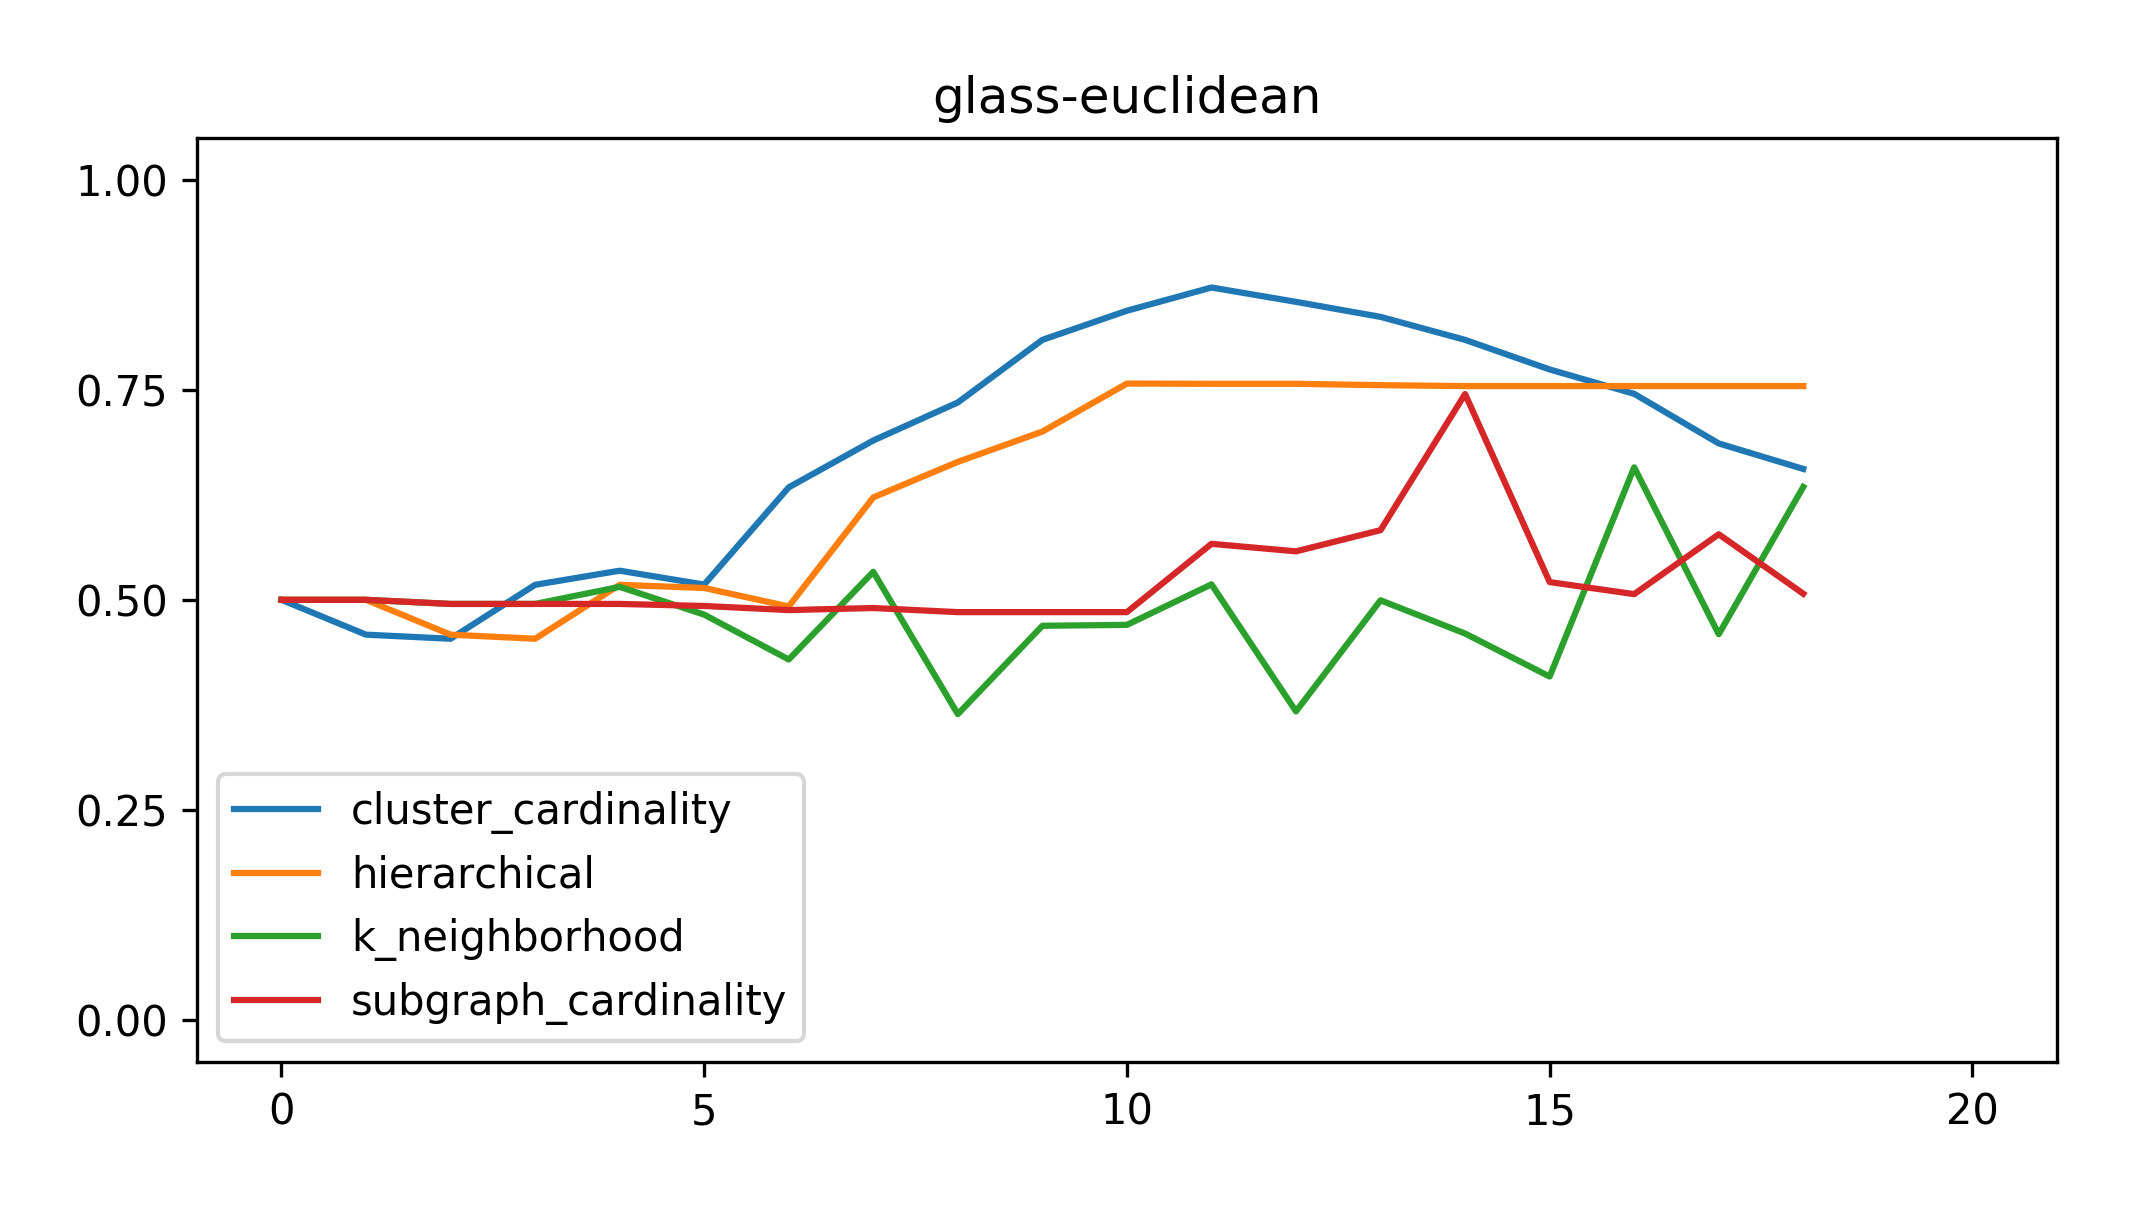
\includegraphics[width=2.2in]{kdd/static/auc_vs_depth/glass-euclidean.png}
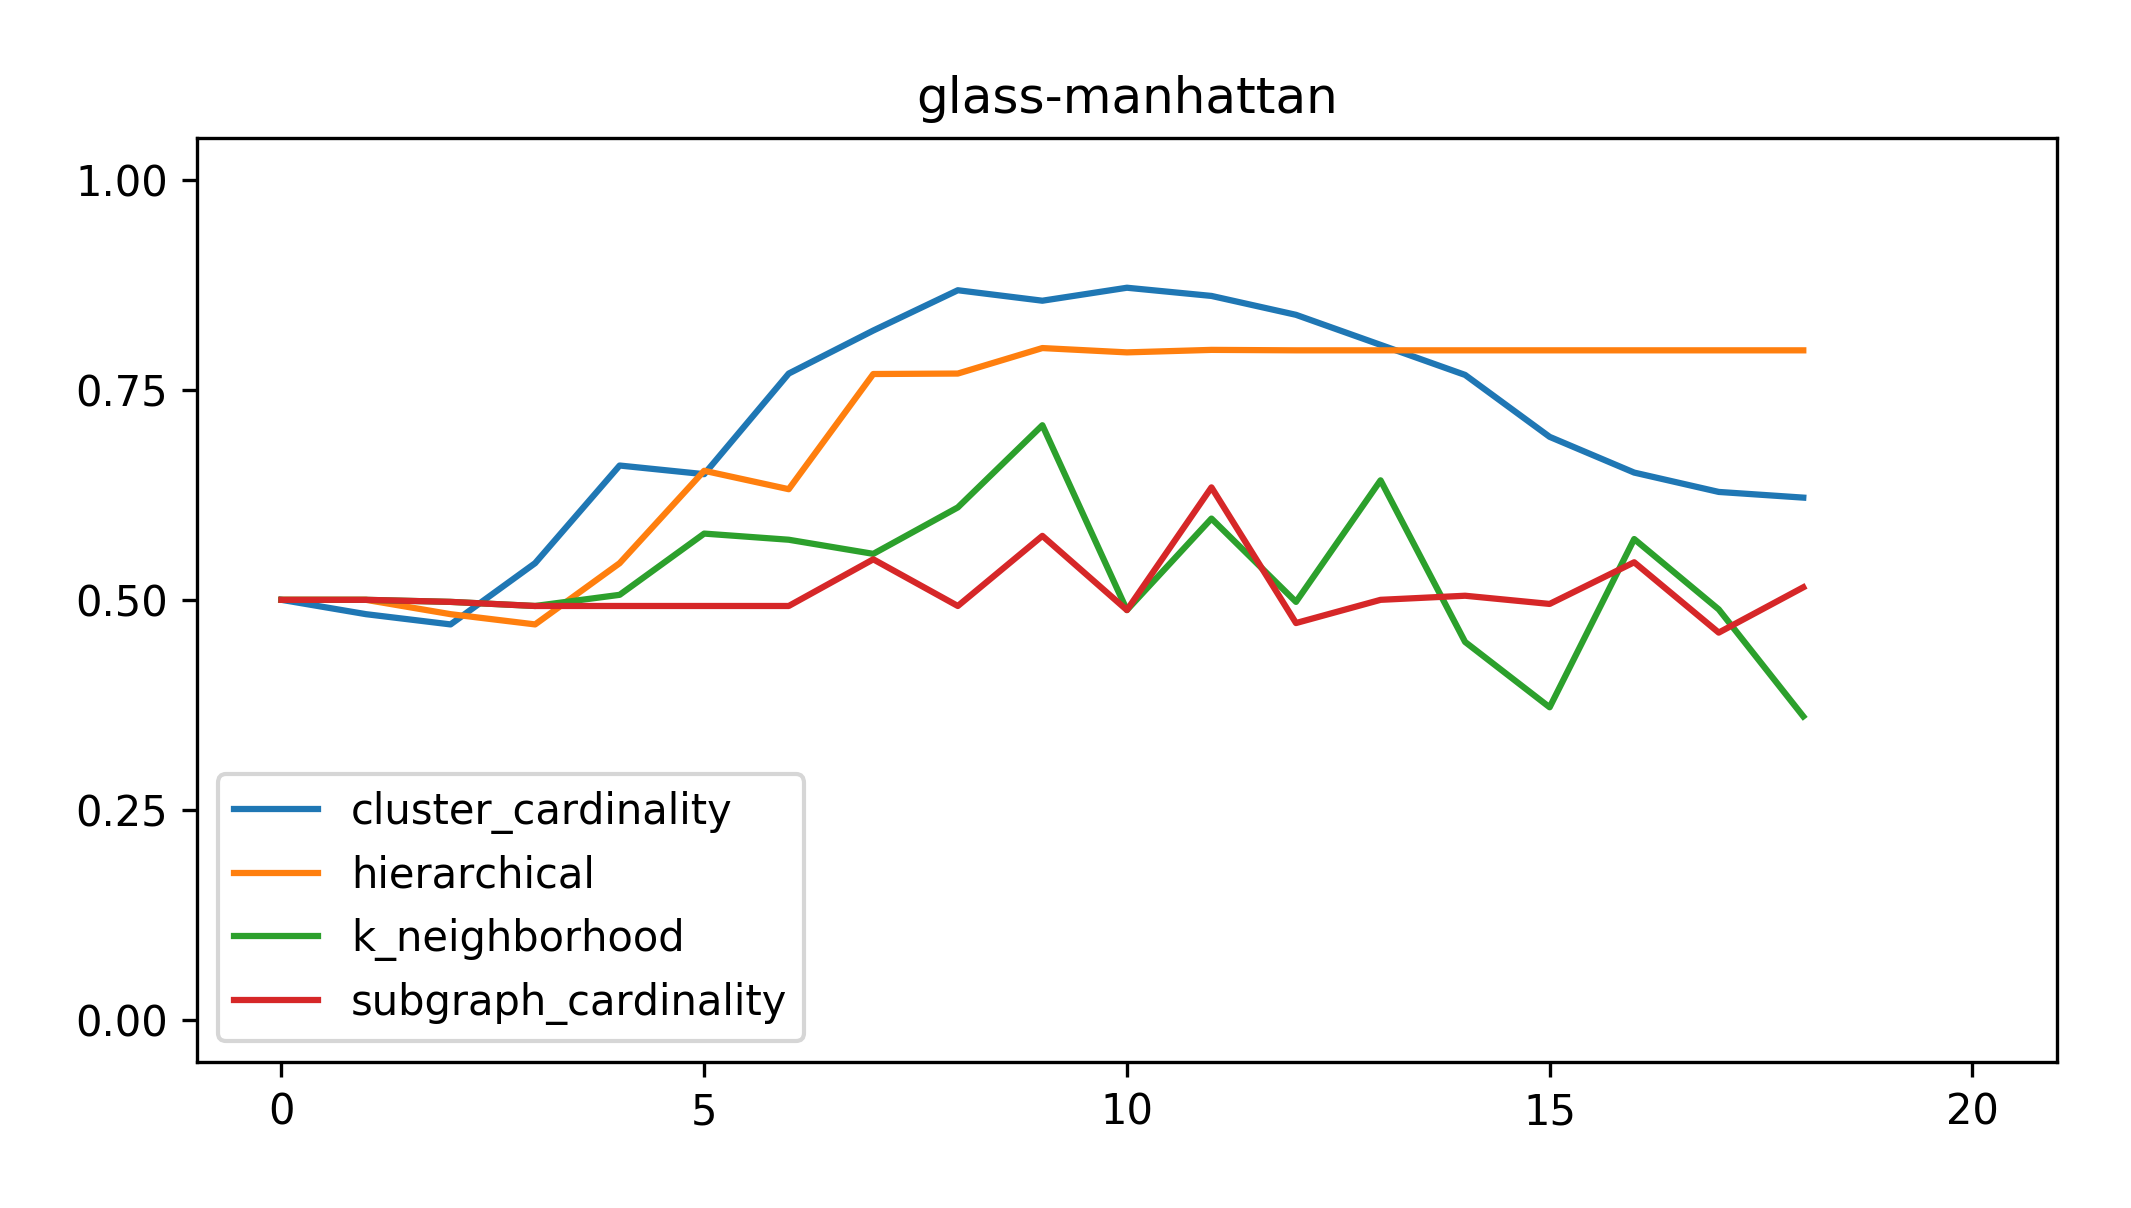
\includegraphics[width=2.2in]{kdd/static/auc_vs_depth/glass-manhattan.png}

% Ionosphere
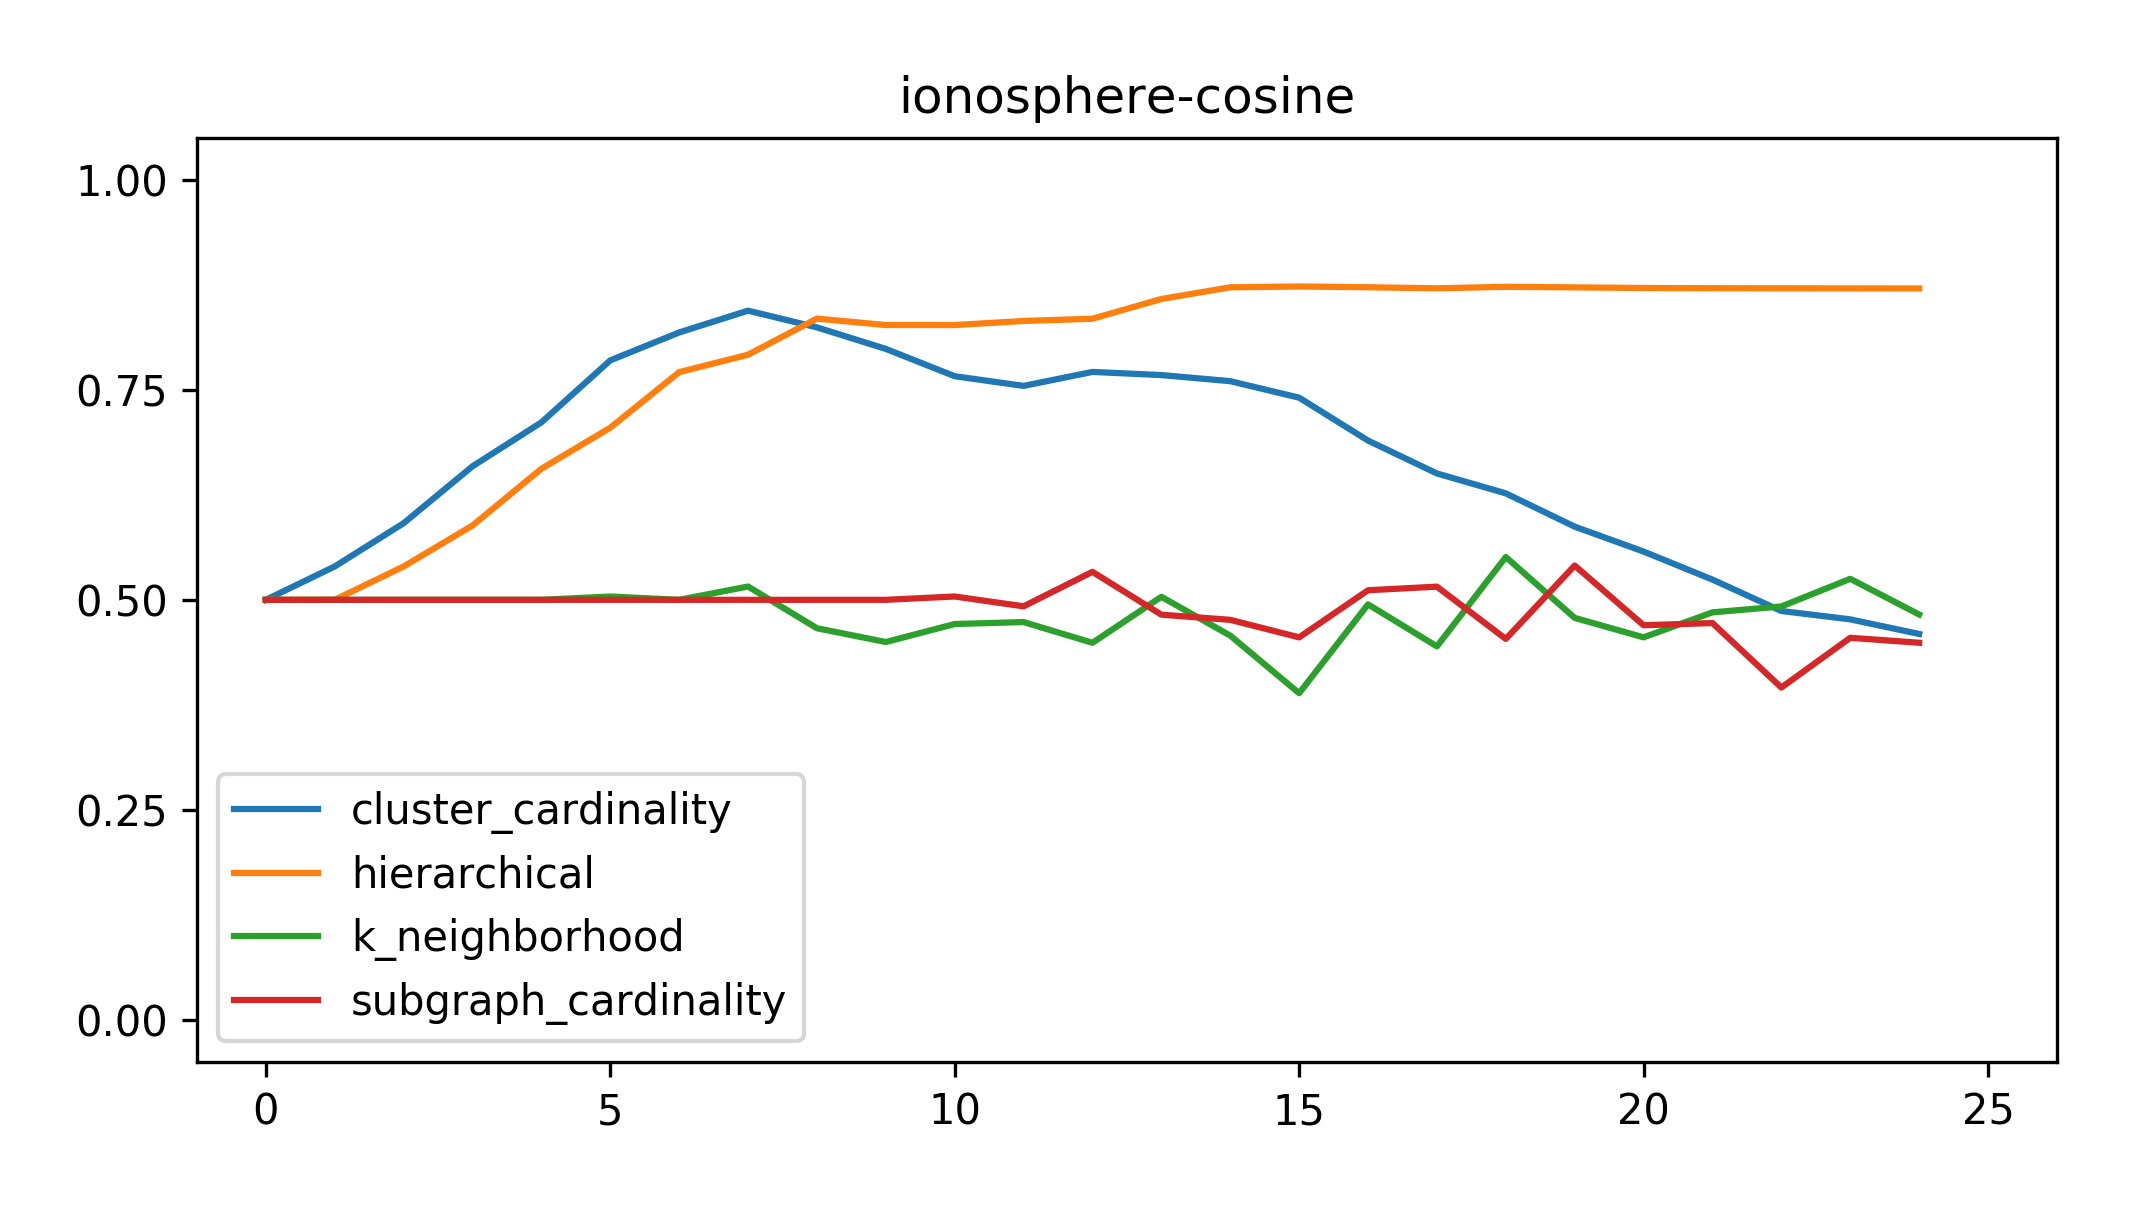
\includegraphics[width=2.2in]{kdd/static/auc_vs_depth/ionosphere-cosine.png}
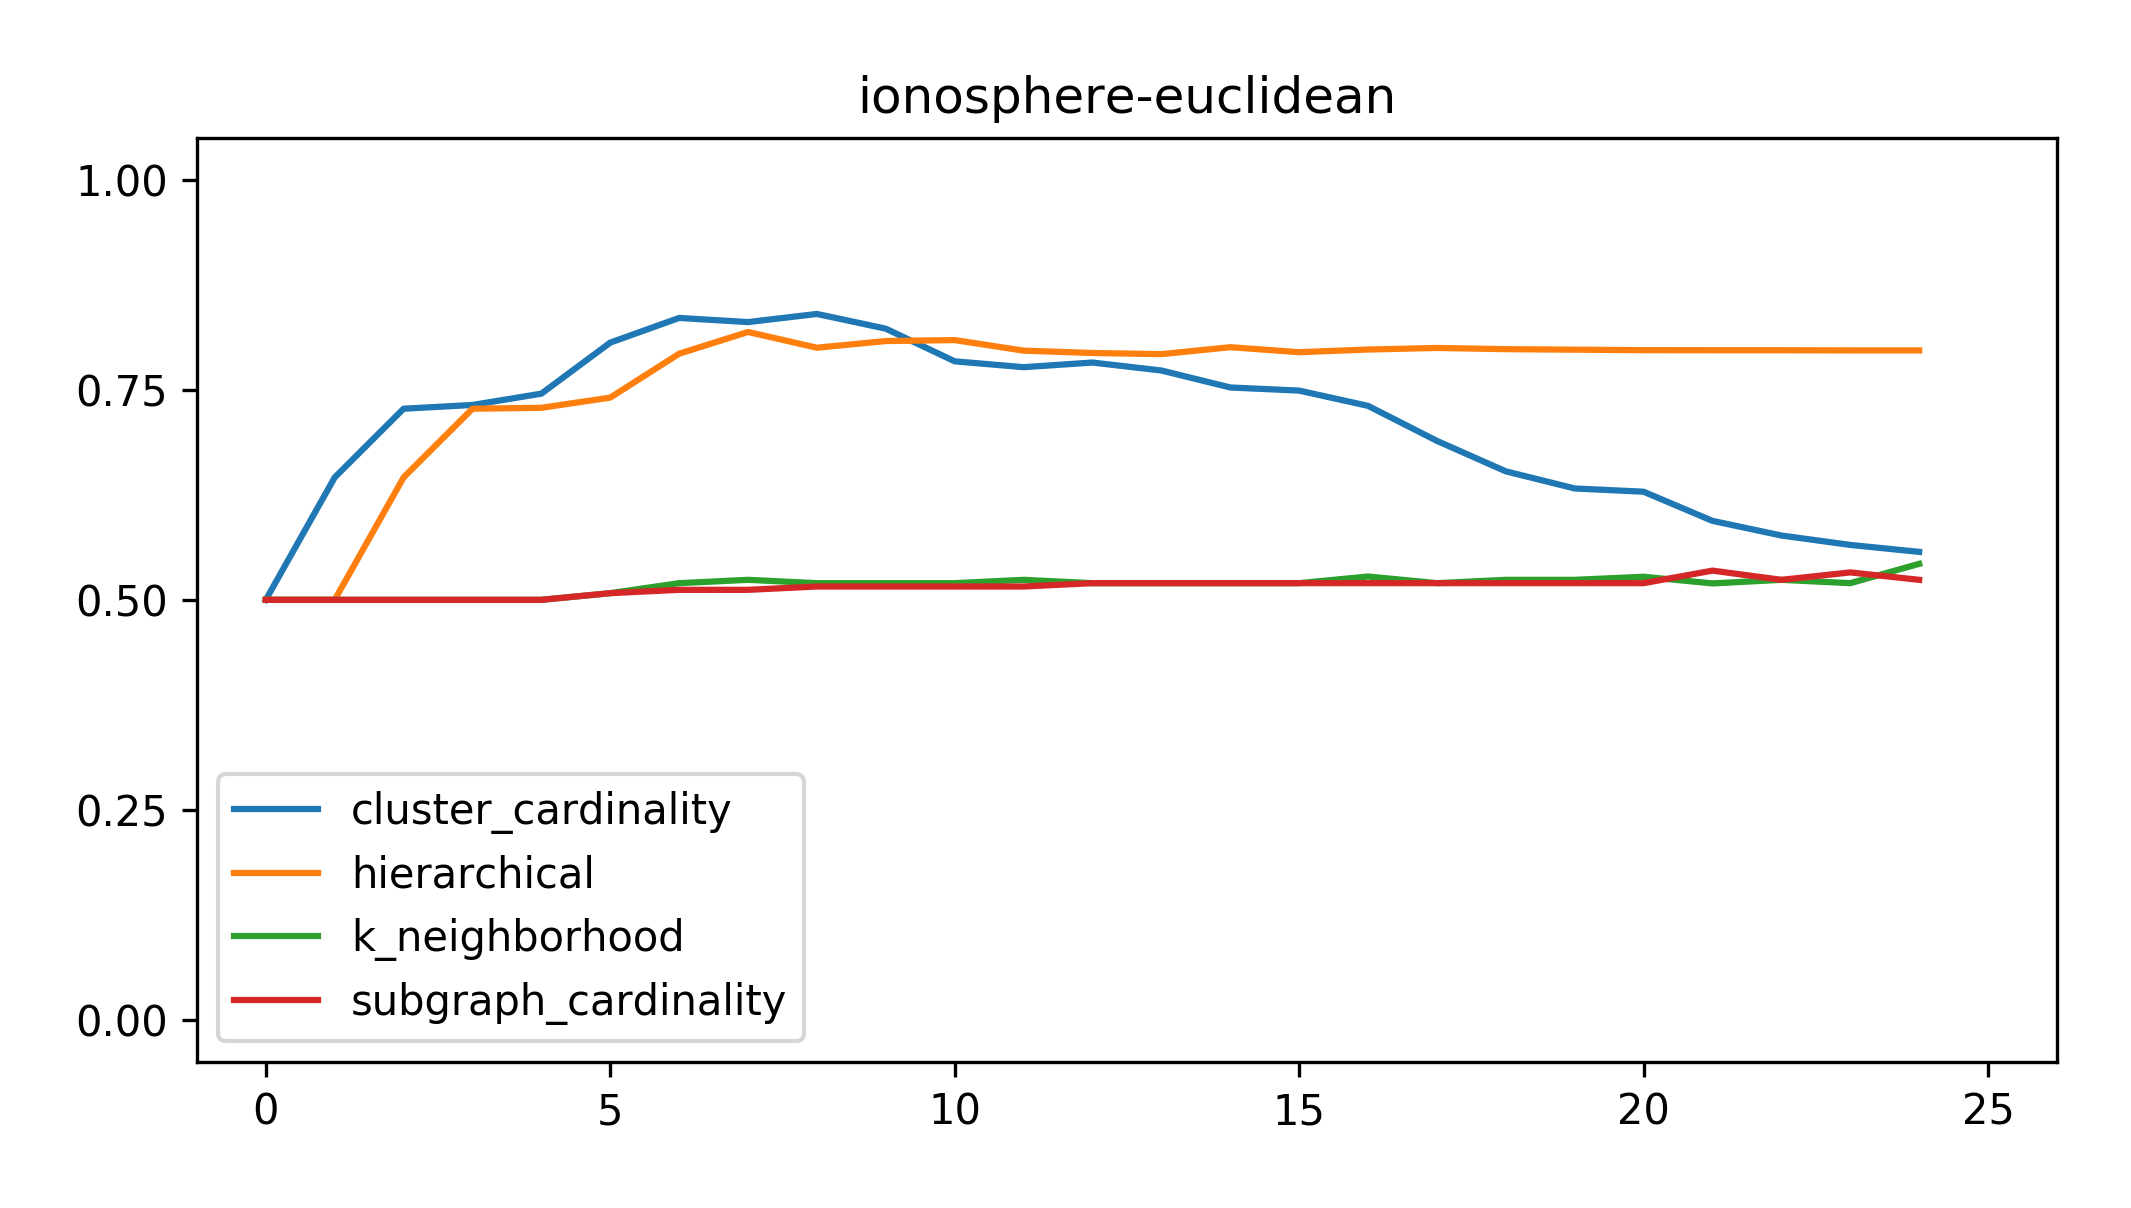
\includegraphics[width=2.2in]{kdd/static/auc_vs_depth/ionosphere-euclidean.png}
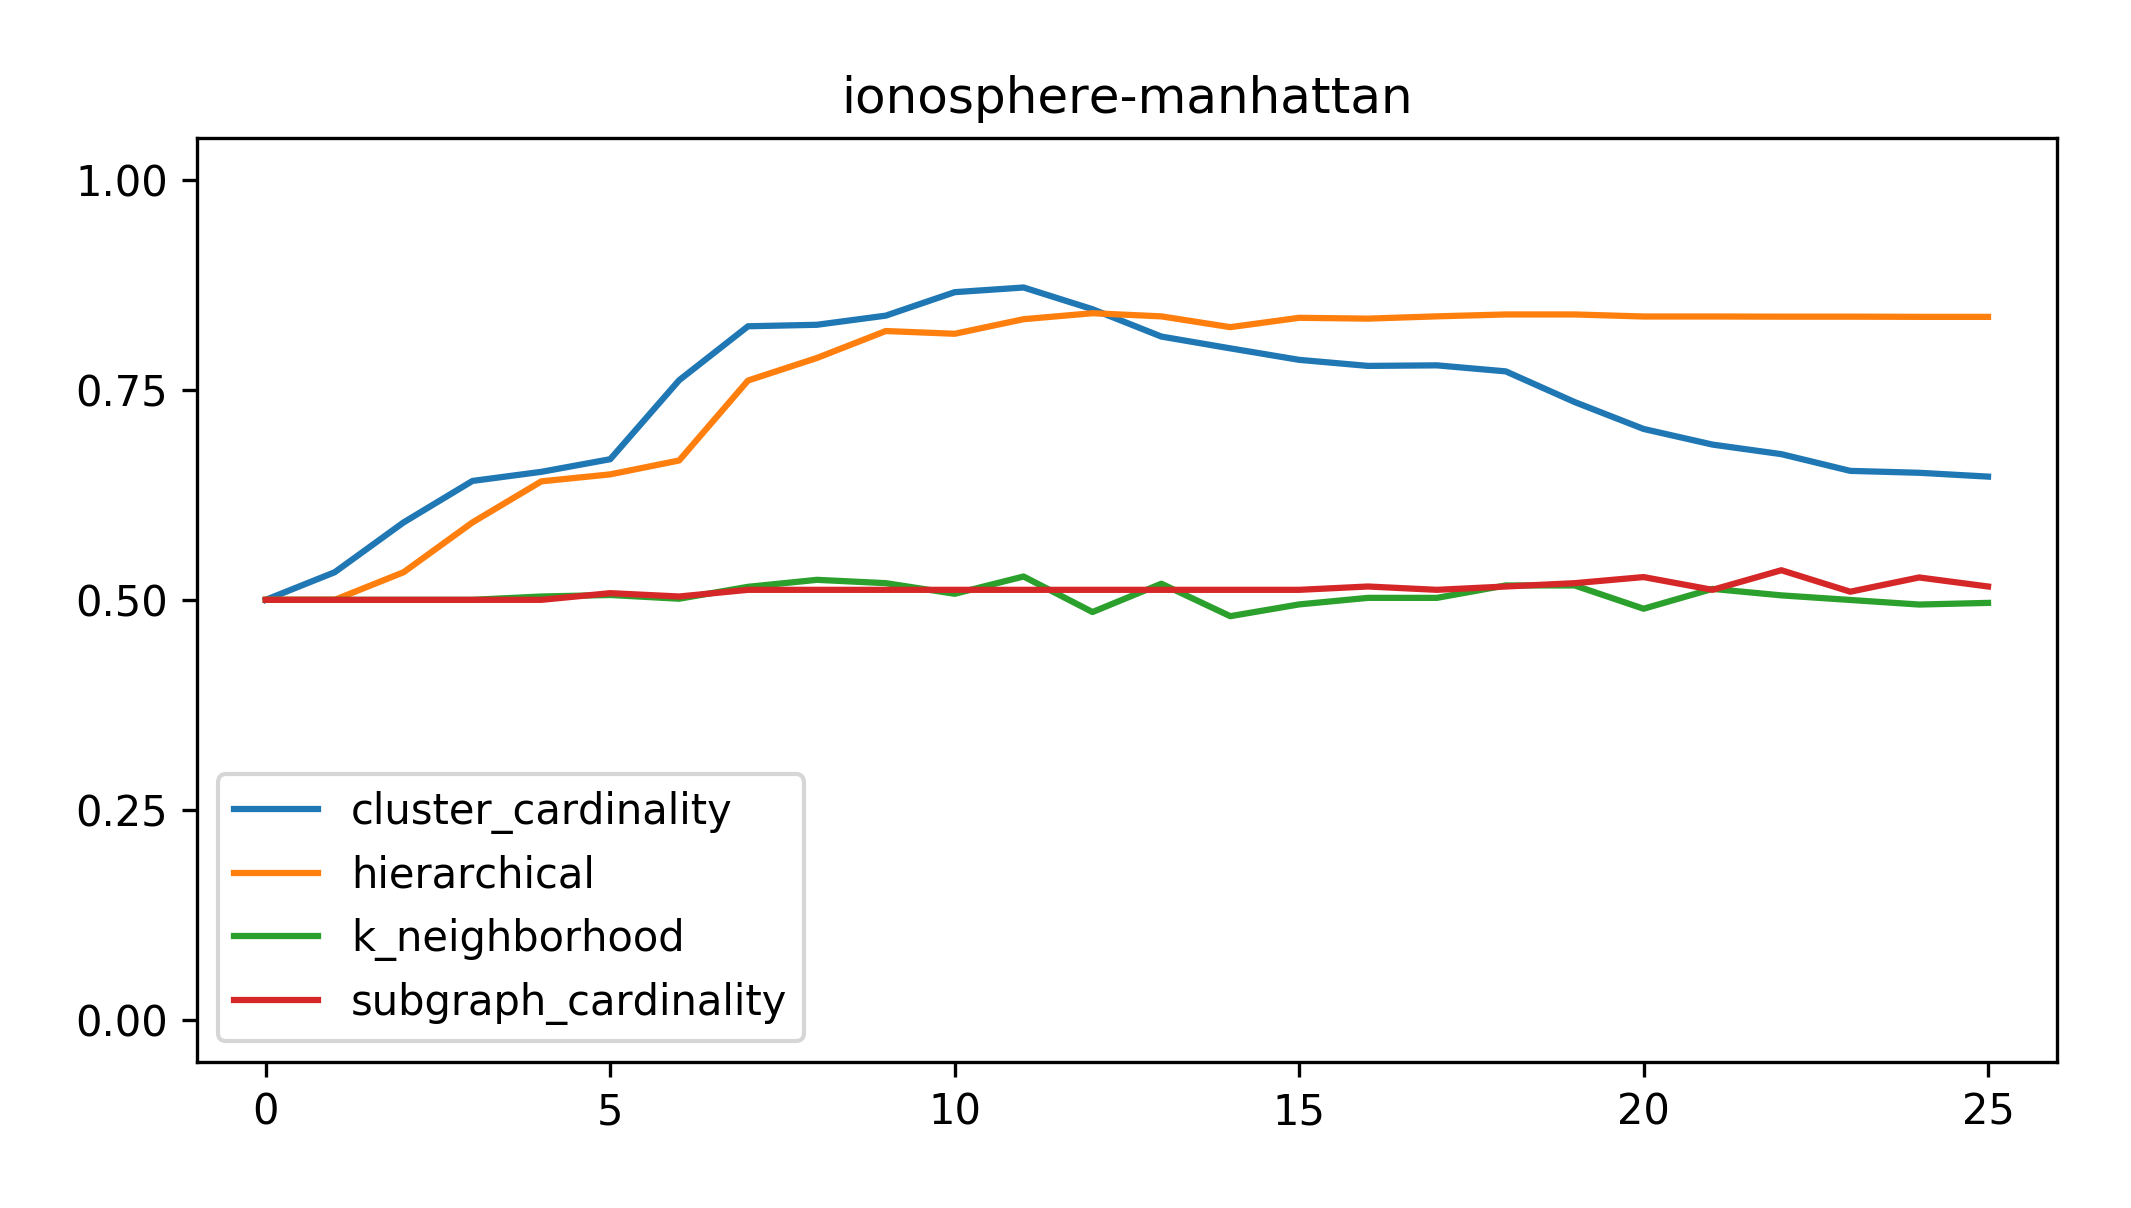
\includegraphics[width=2.2in]{kdd/static/auc_vs_depth/ionosphere-manhattan.png}

\caption{
Plots of ROC-AUC vs Depth for our measures of Anomolousness.
}

\label{results:datasets_1}
\end{figure*}

\begin{figure*}[!t]
\centering
% Lympho
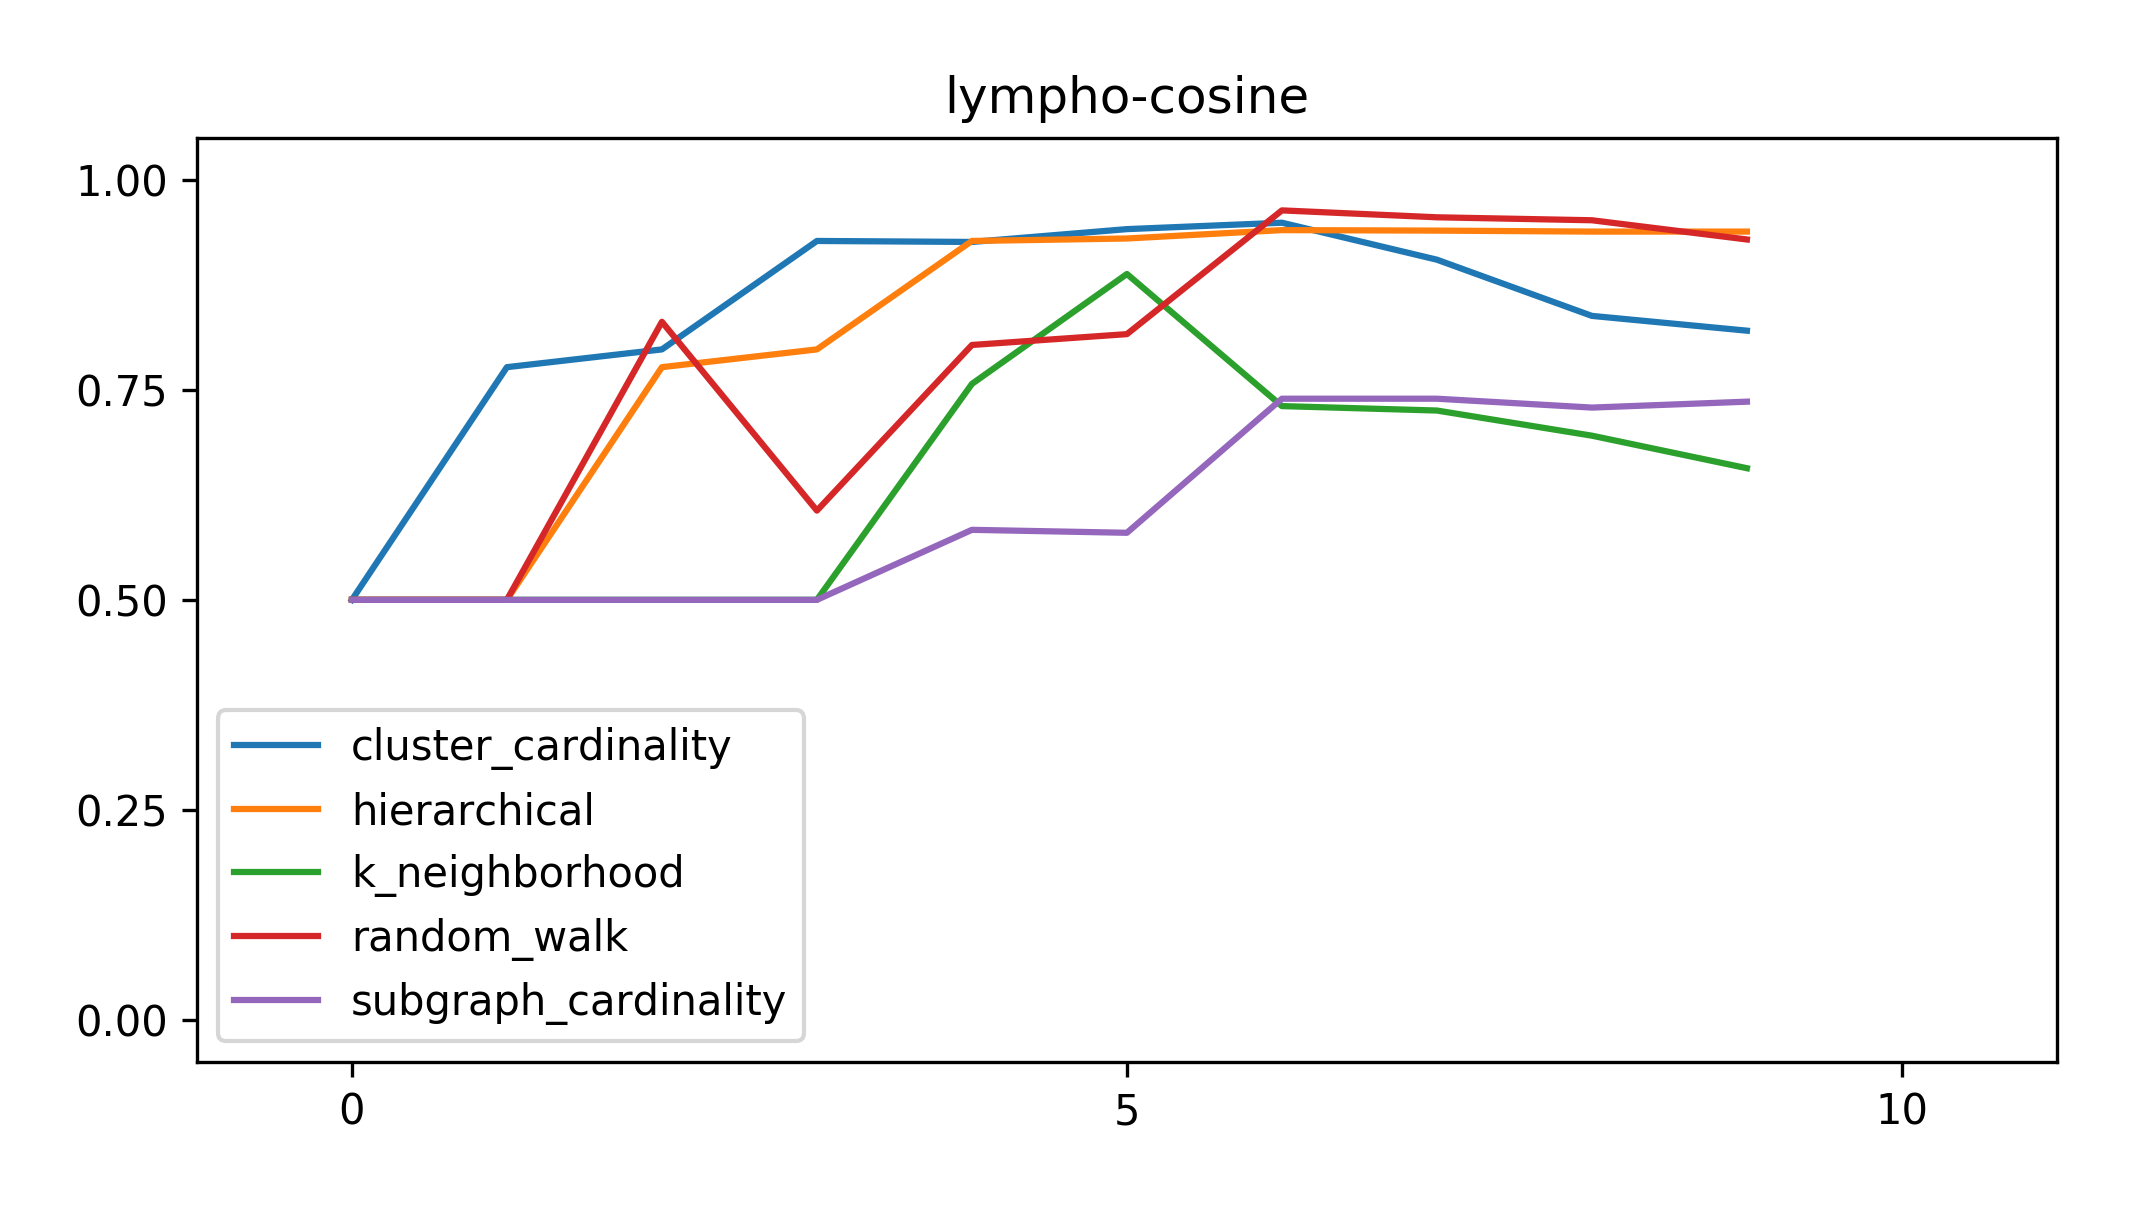
\includegraphics[width=2.2in]{kdd/static/auc_vs_depth/lympho-cosine.png}
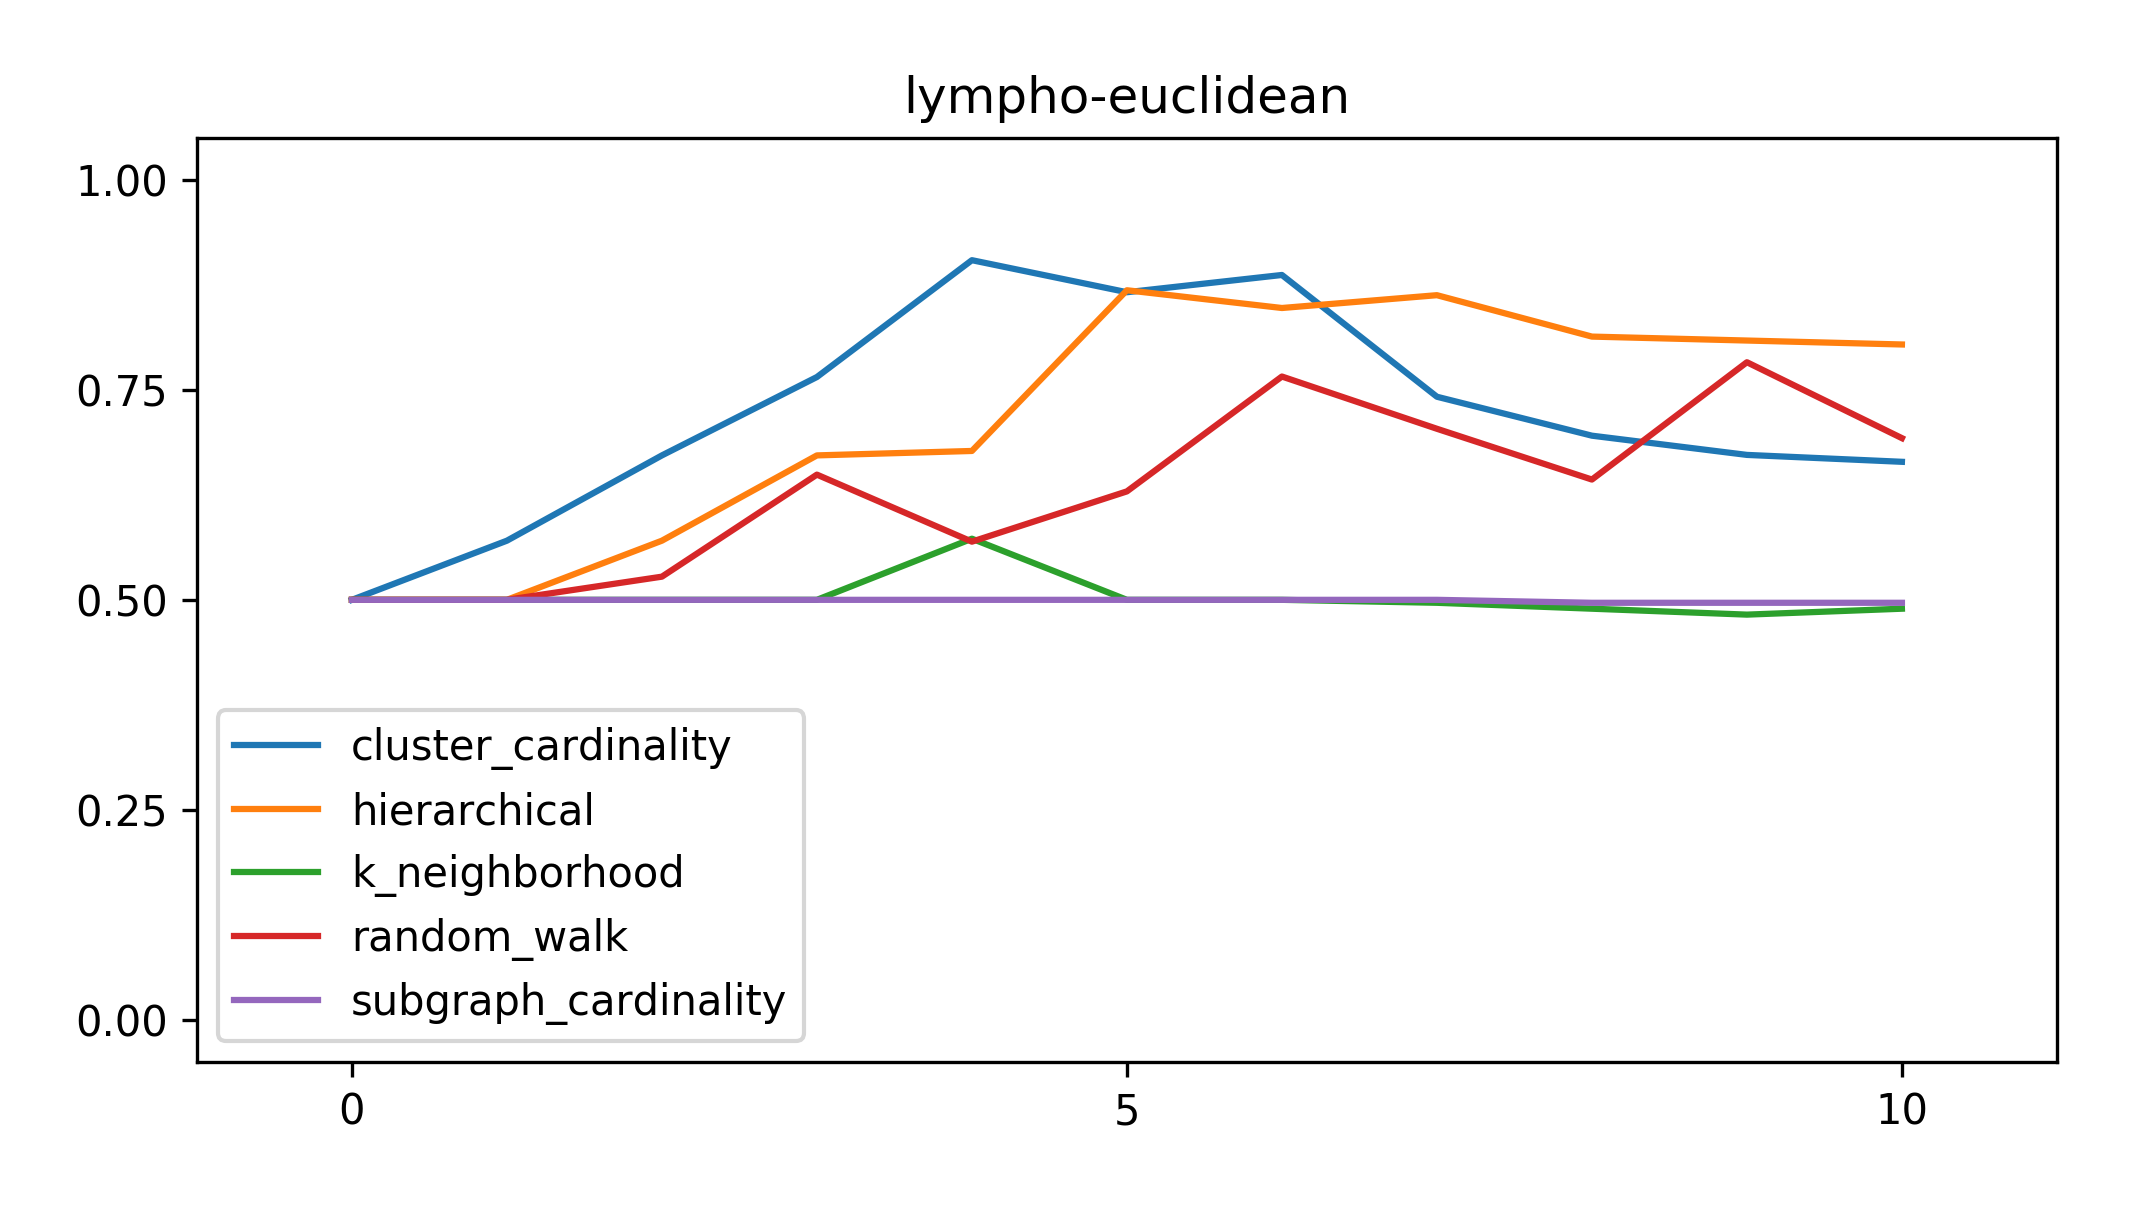
\includegraphics[width=2.2in]{kdd/static/auc_vs_depth/lympho-euclidean.png}
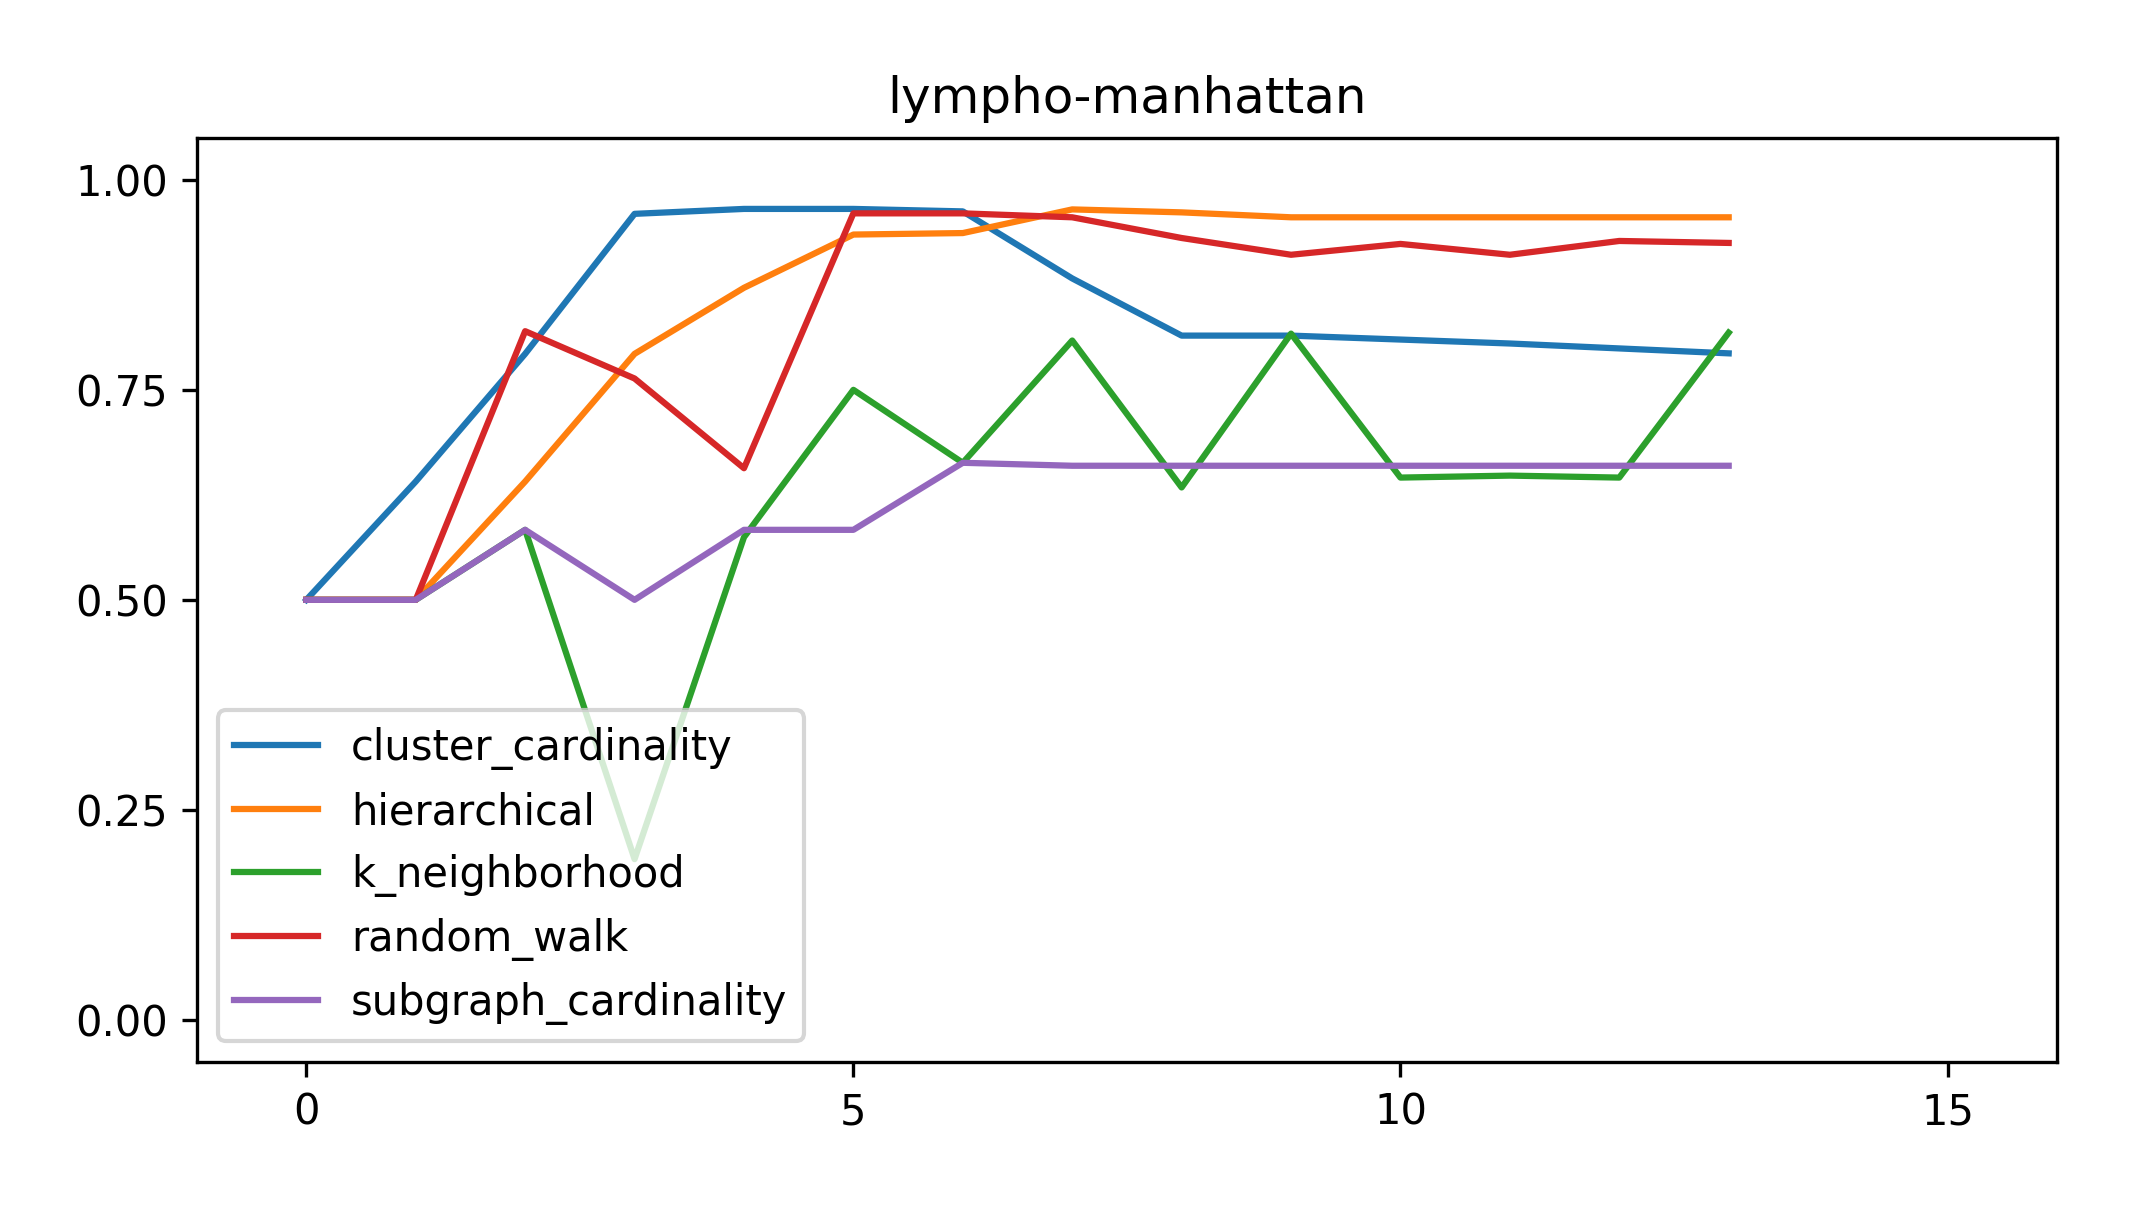
\includegraphics[width=2.2in]{kdd/static/auc_vs_depth/lympho-manhattan.png}

% Mnist
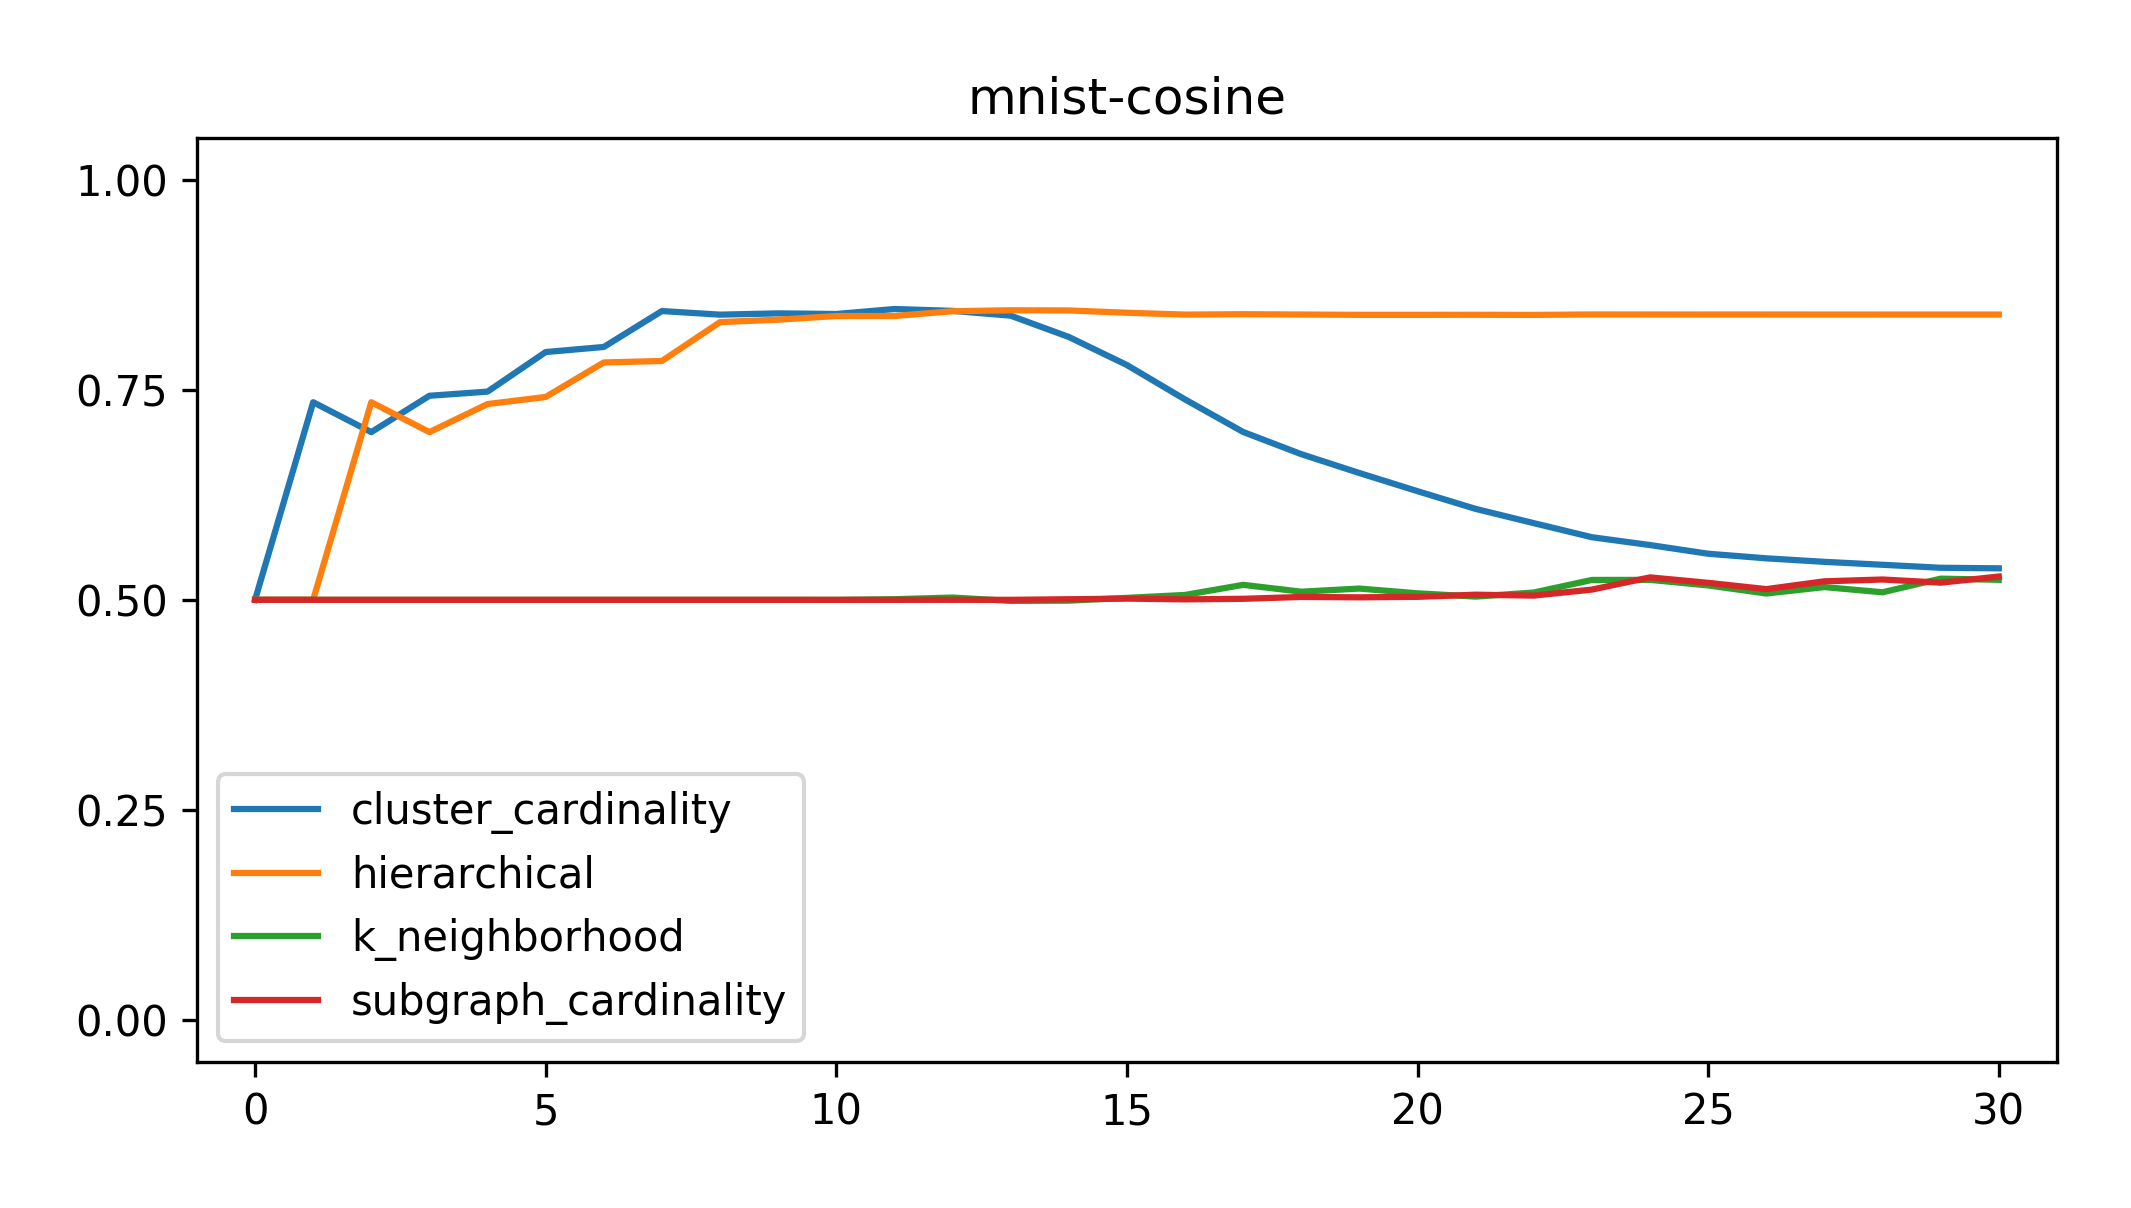
\includegraphics[width=2.2in]{kdd/static/auc_vs_depth/mnist-cosine.png}
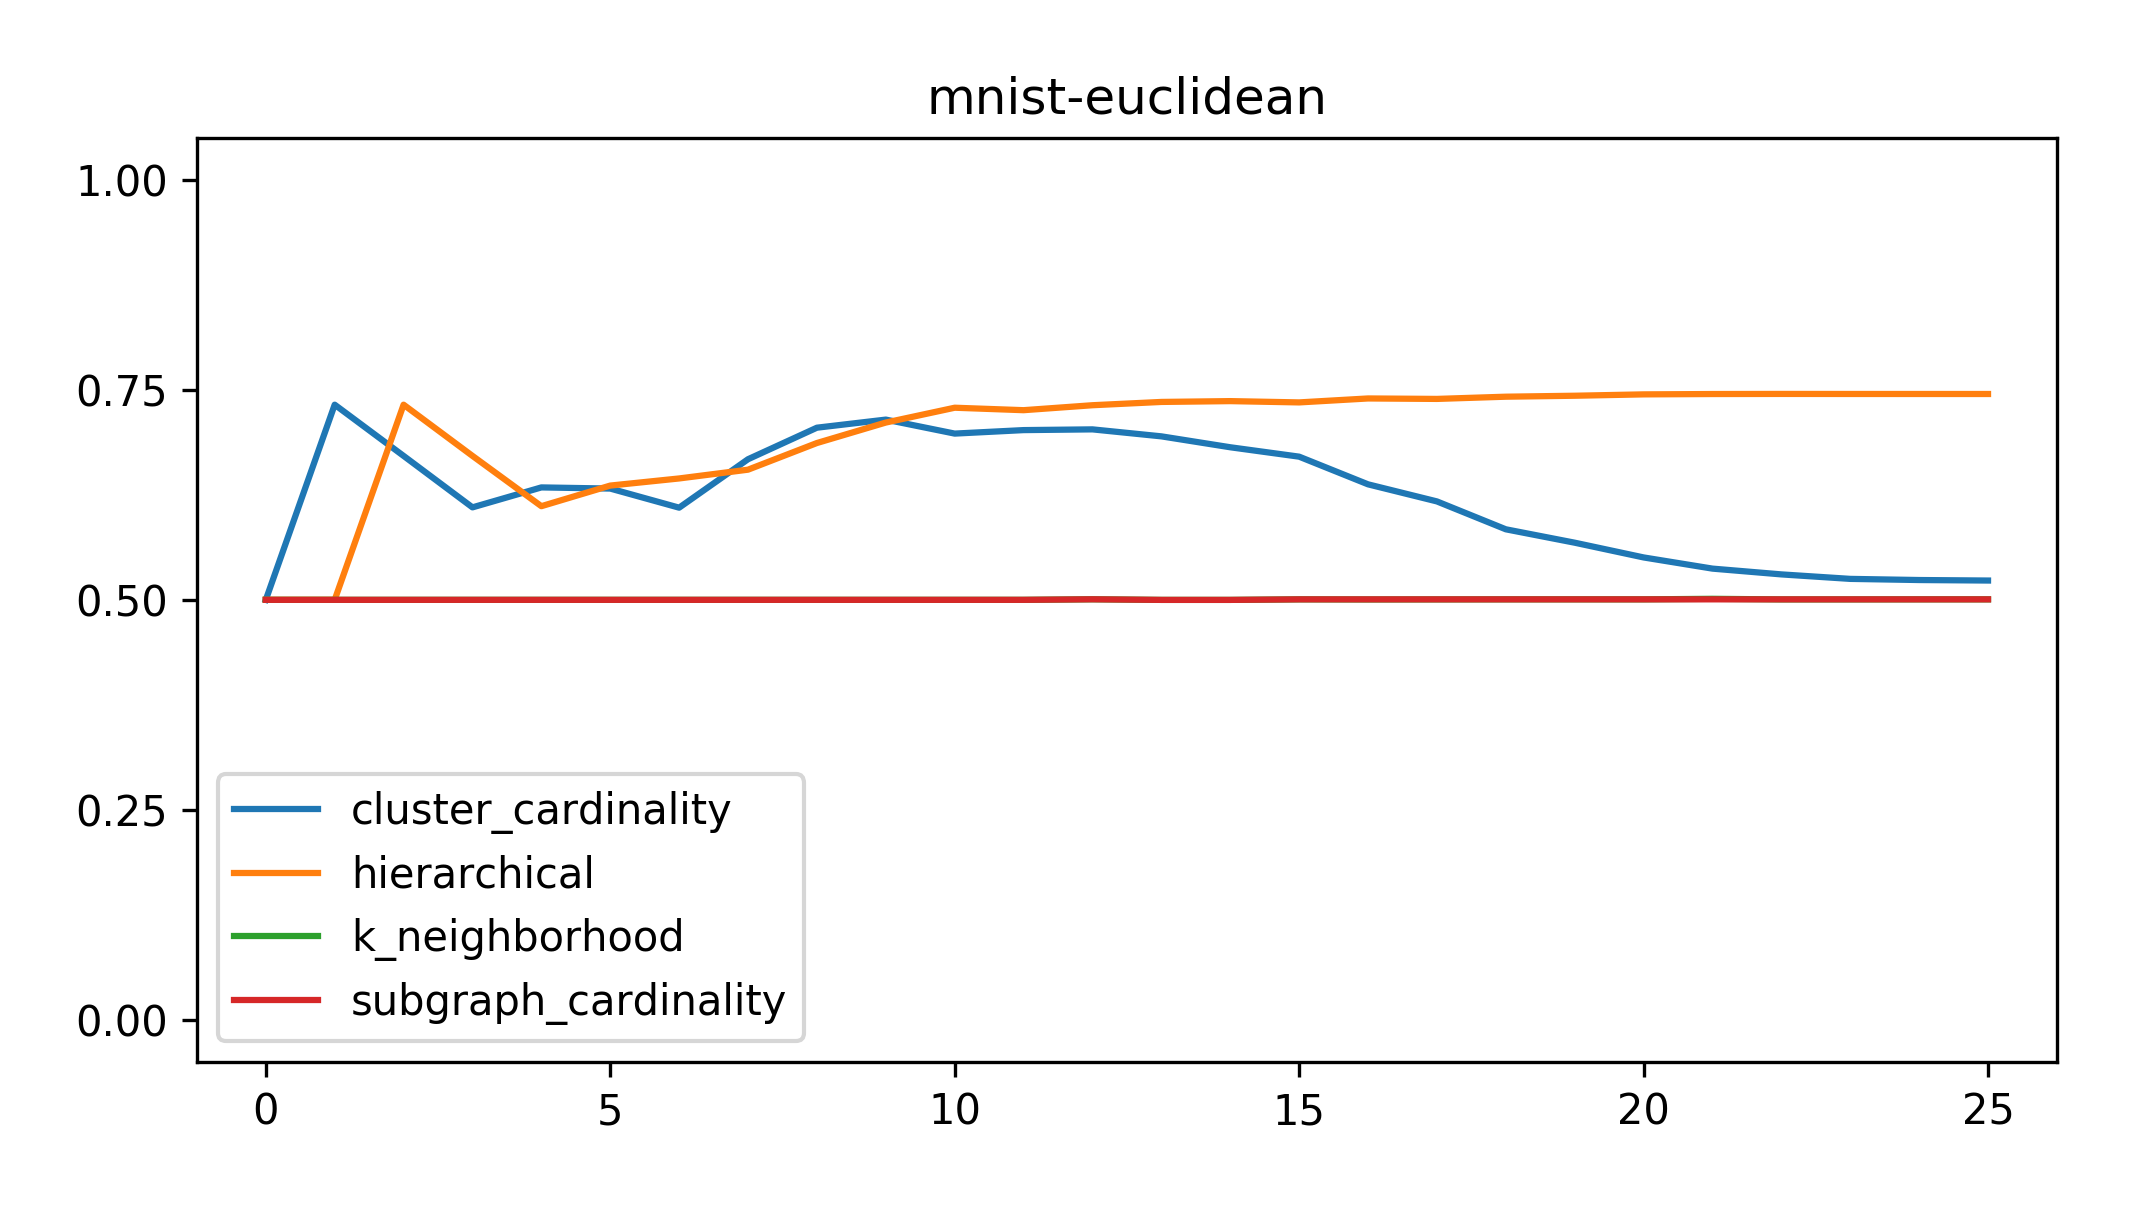
\includegraphics[width=2.2in]{kdd/static/auc_vs_depth/mnist-euclidean.png}
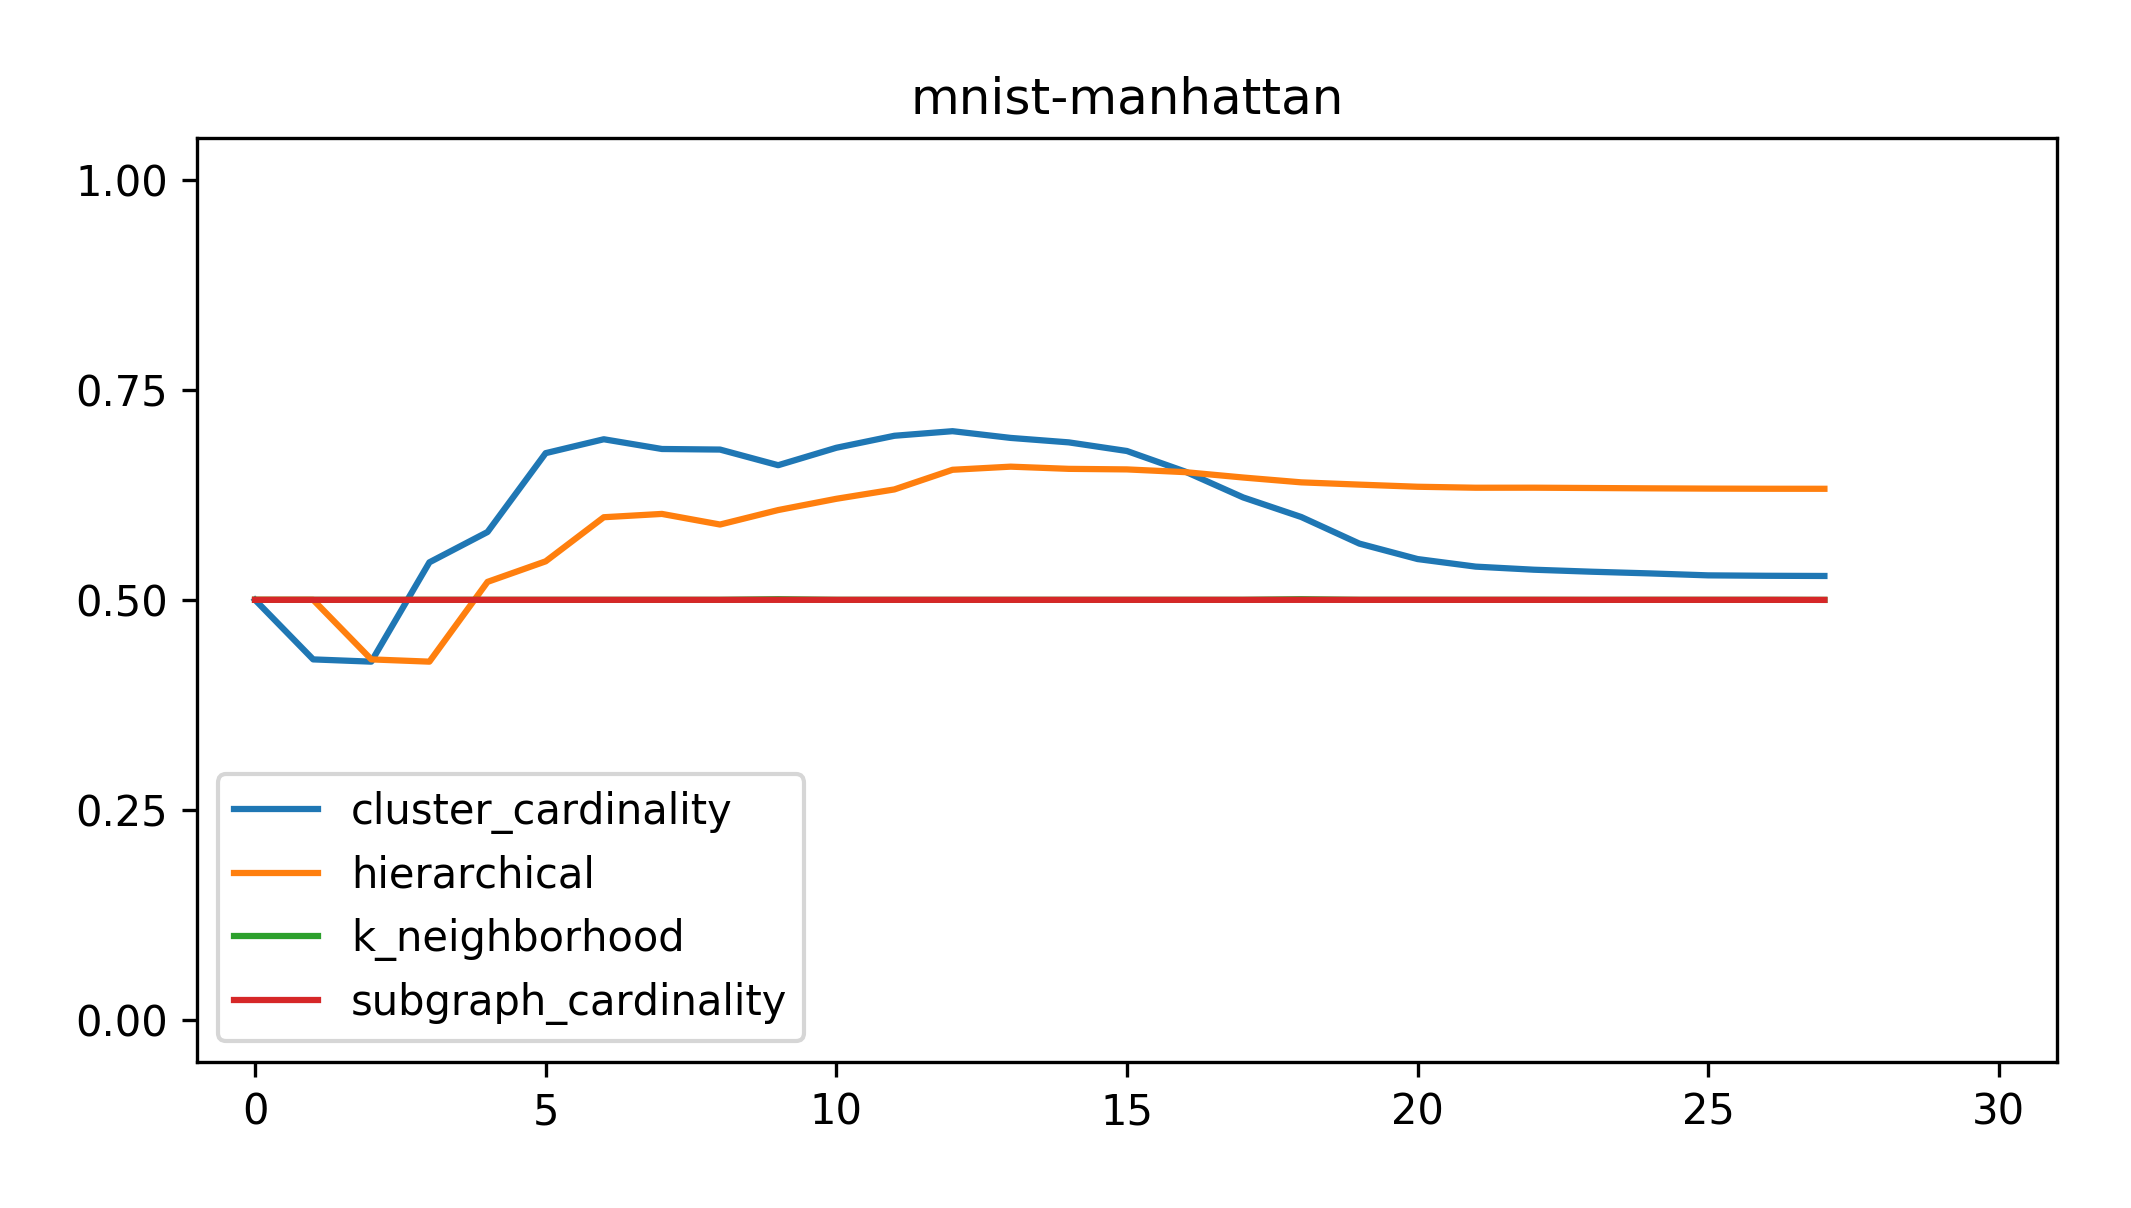
\includegraphics[width=2.2in]{kdd/static/auc_vs_depth/mnist-manhattan.png}

% Musk
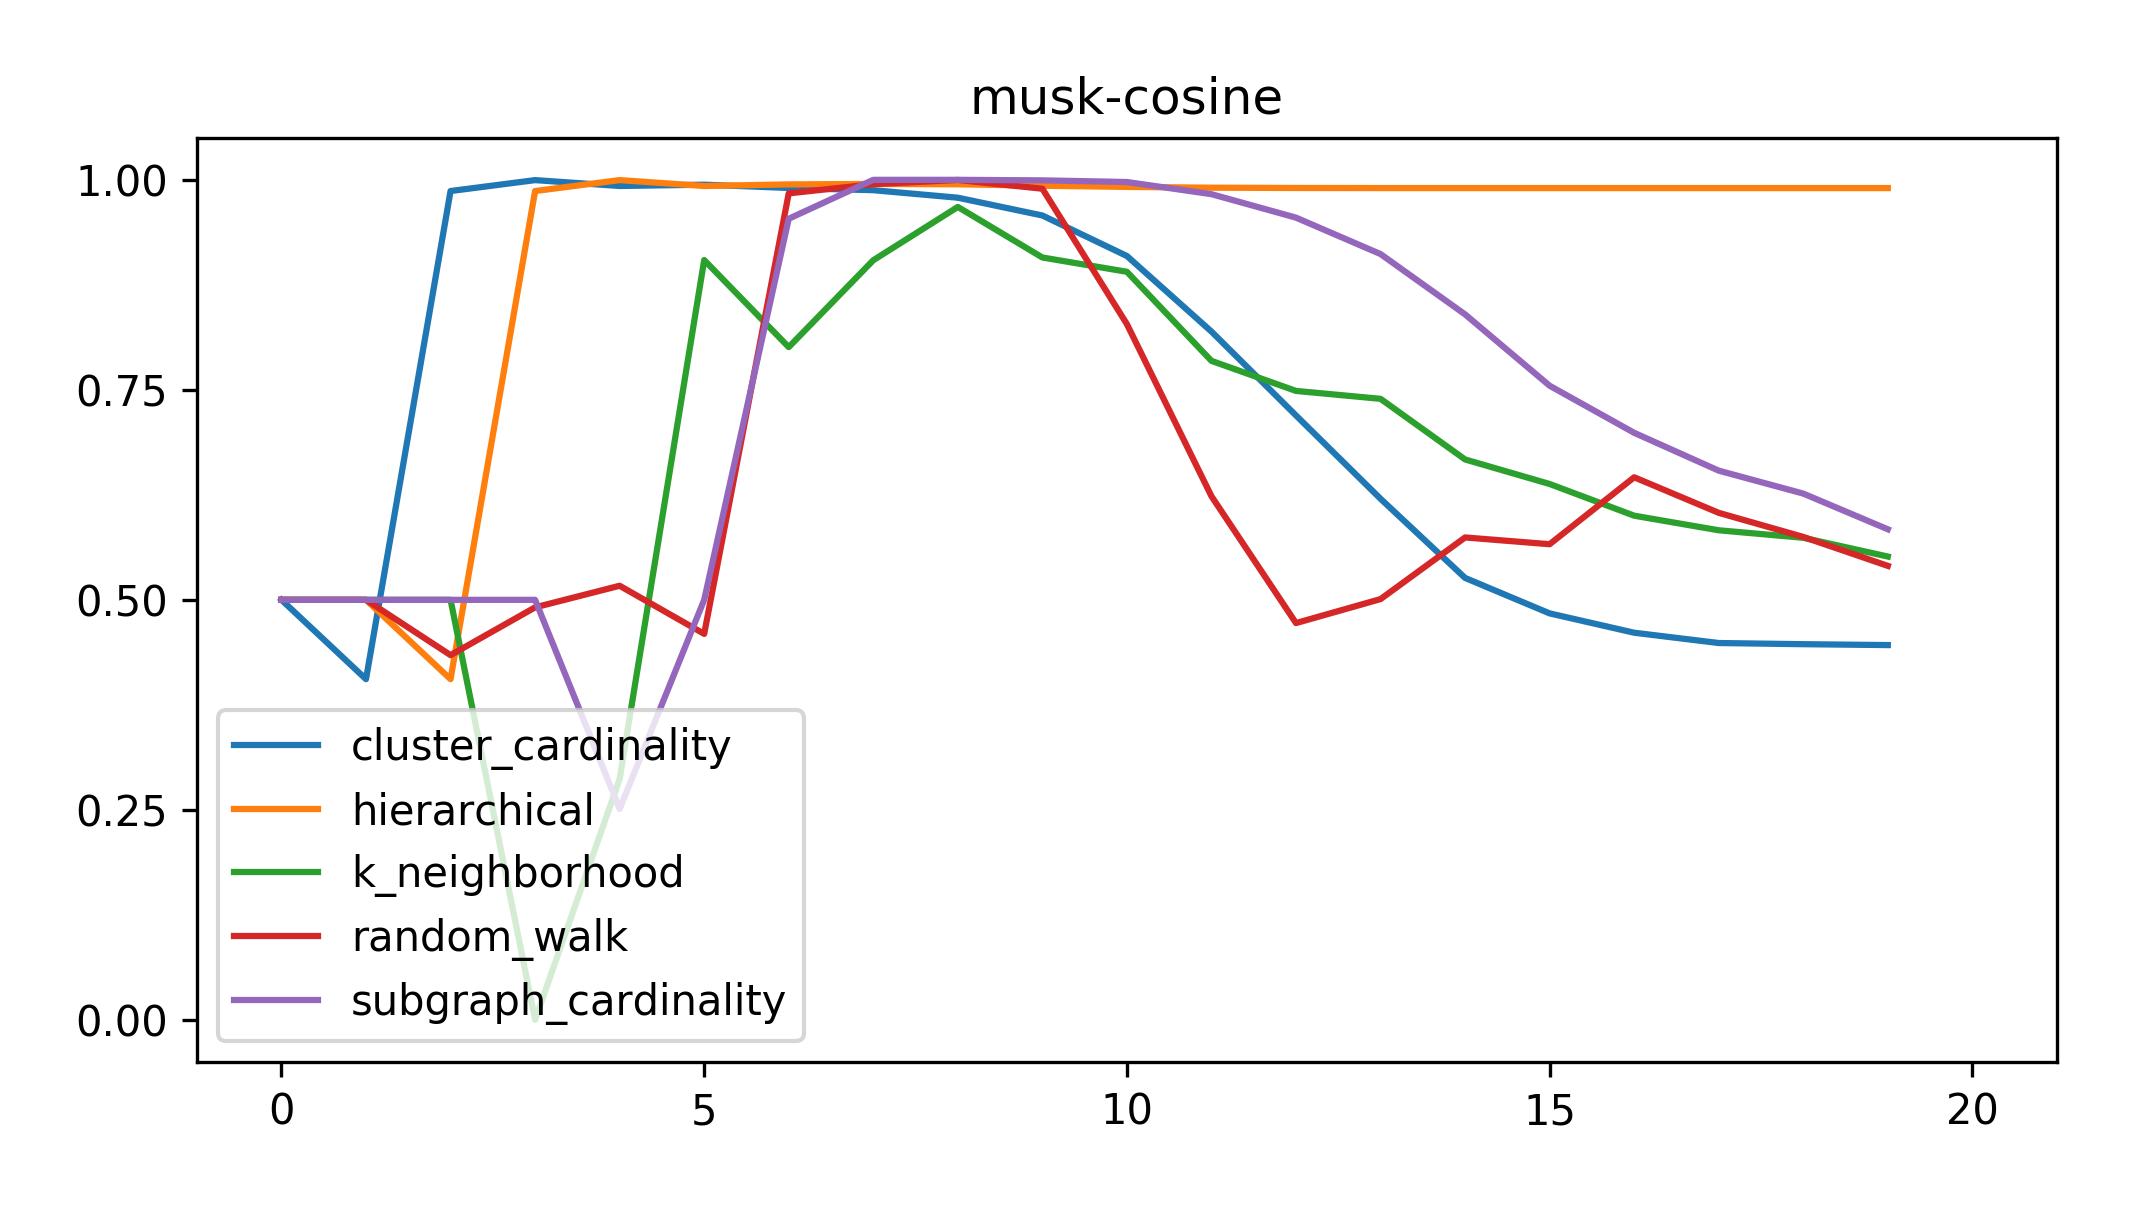
\includegraphics[width=2.2in]{kdd/static/auc_vs_depth/musk-cosine.png}
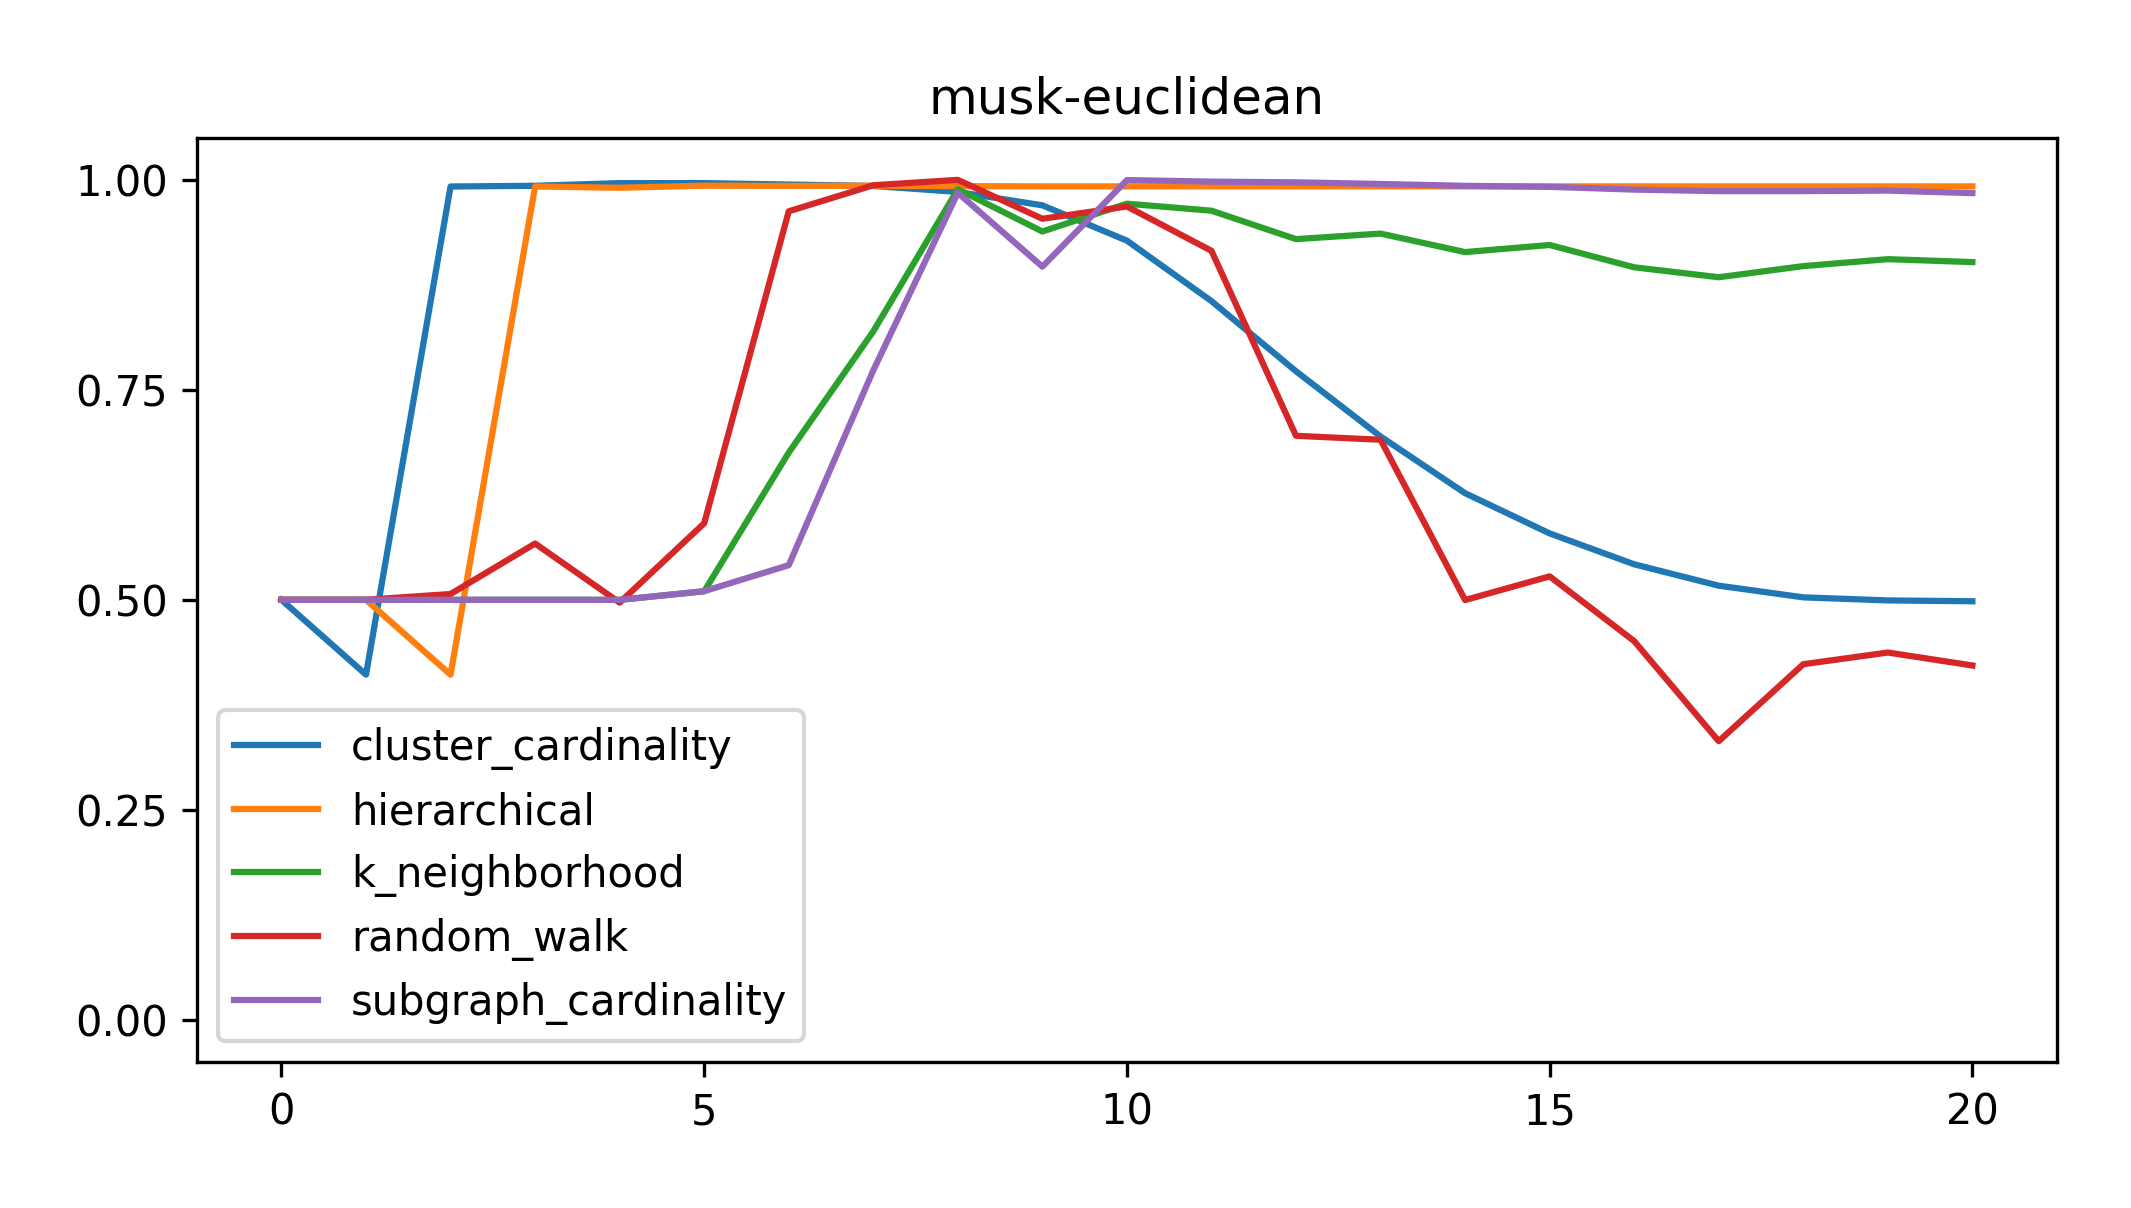
\includegraphics[width=2.2in]{kdd/static/auc_vs_depth/musk-euclidean.png}
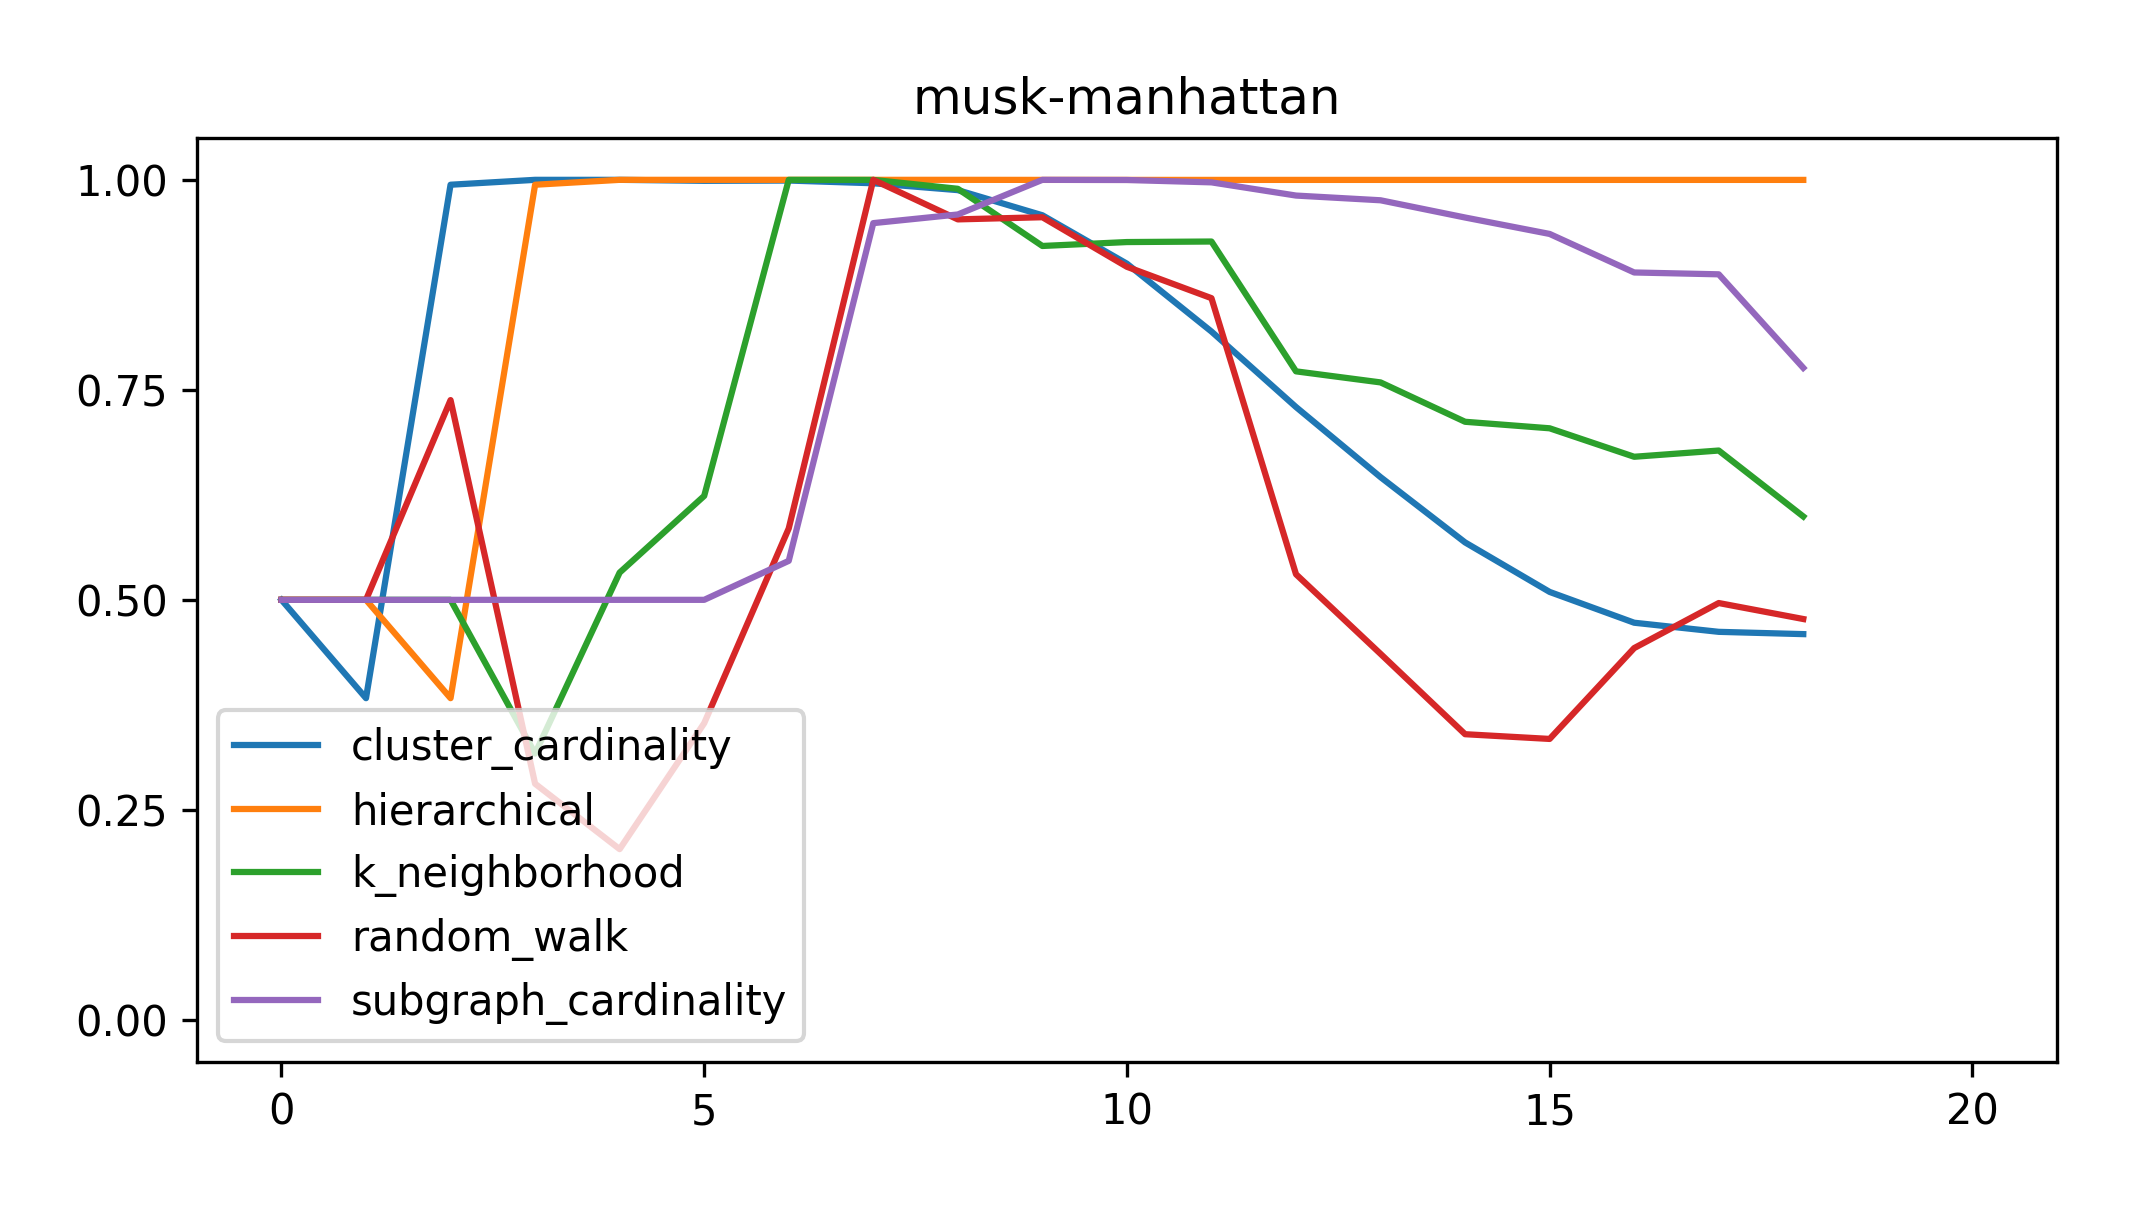
\includegraphics[width=2.2in]{kdd/static/auc_vs_depth/musk-manhattan.png}

% Optdigits
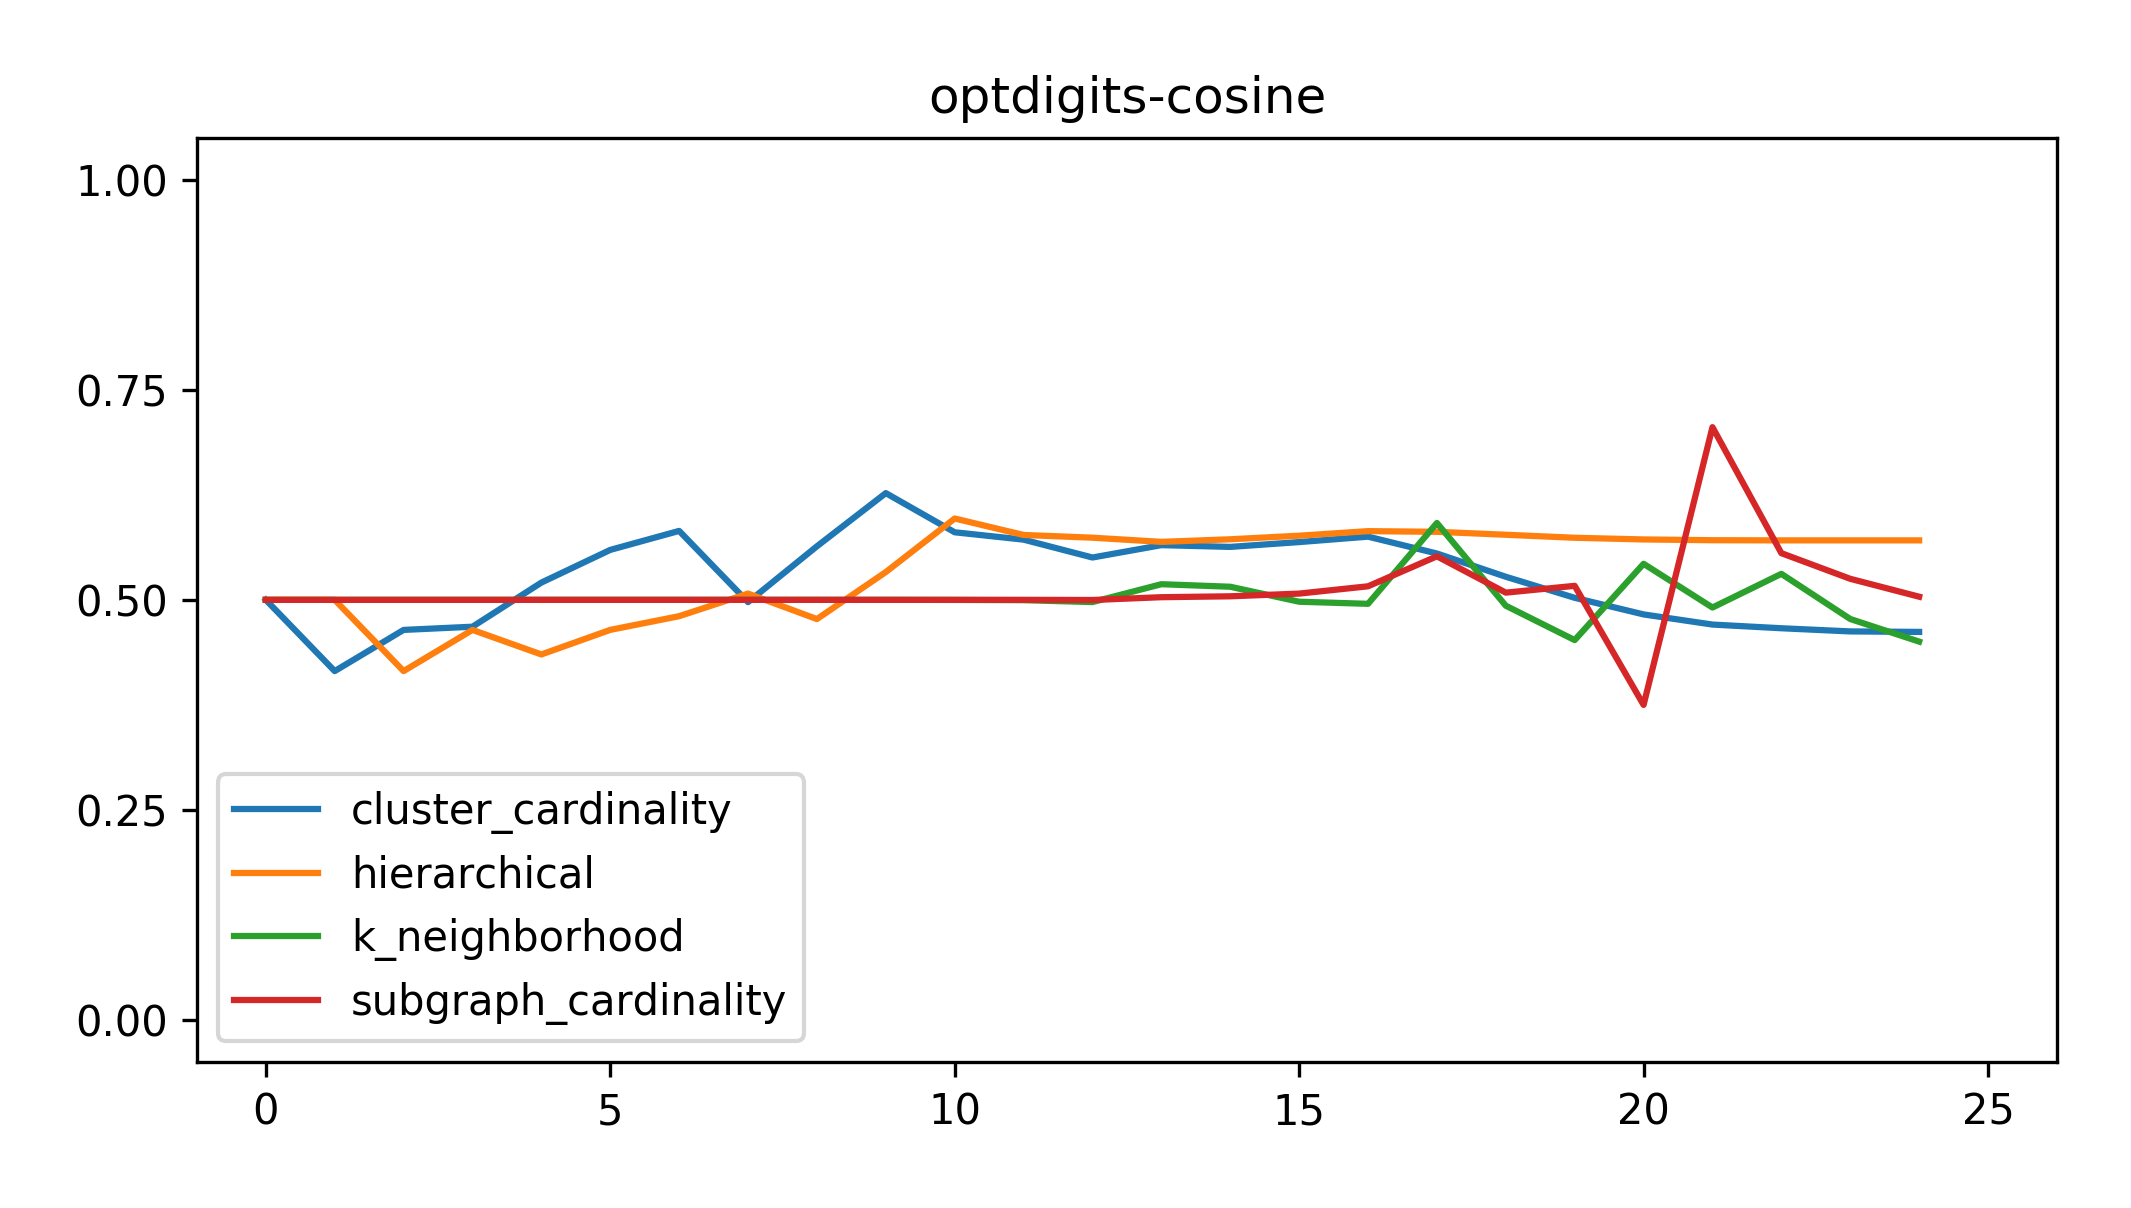
\includegraphics[width=2.2in]{kdd/static/auc_vs_depth/optdigits-cosine.png}
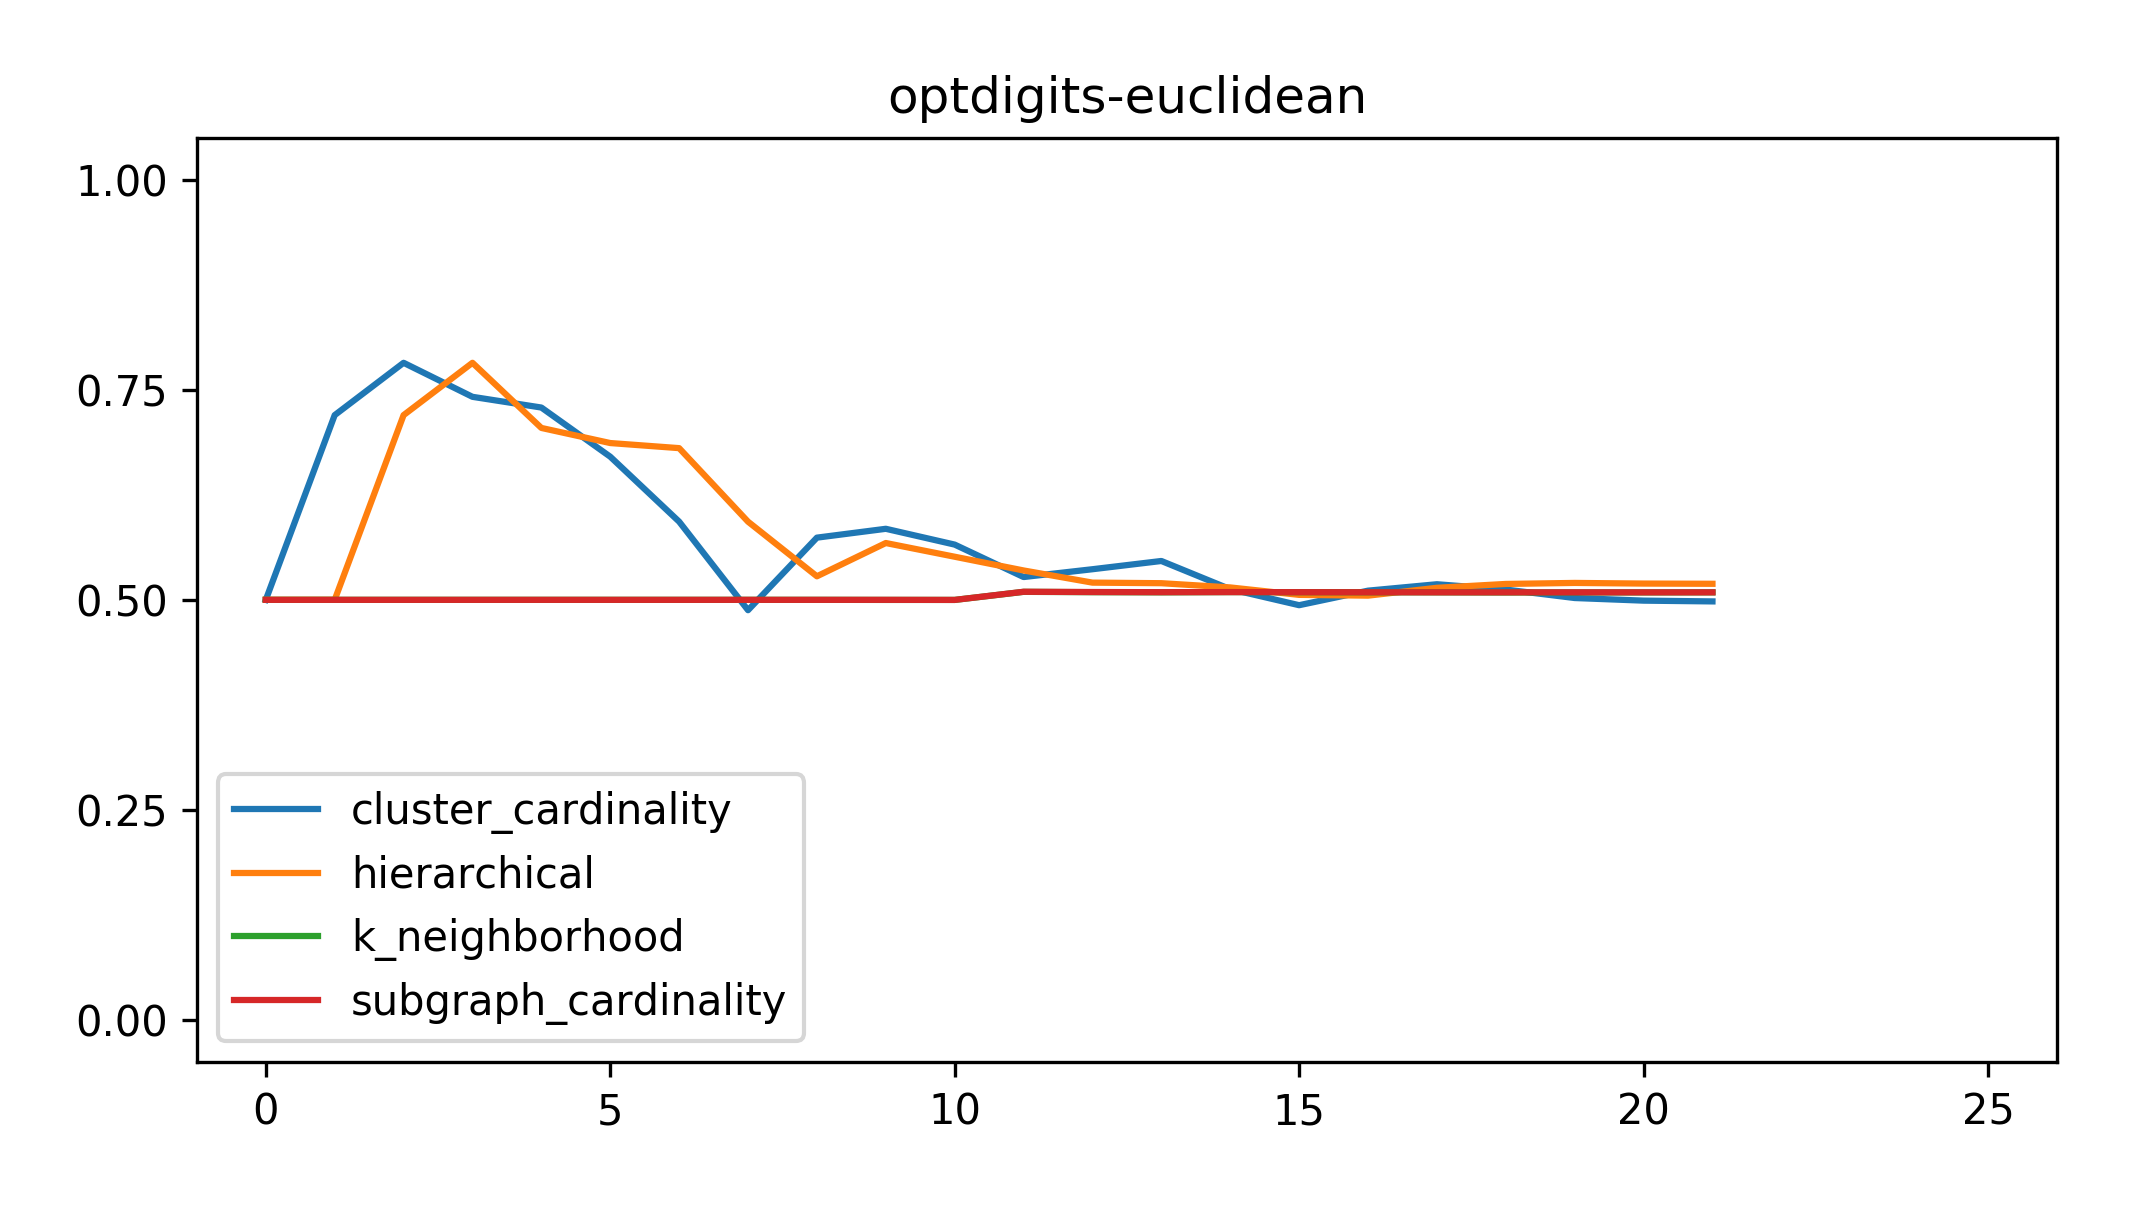
\includegraphics[width=2.2in]{kdd/static/auc_vs_depth/optdigits-euclidean.png}
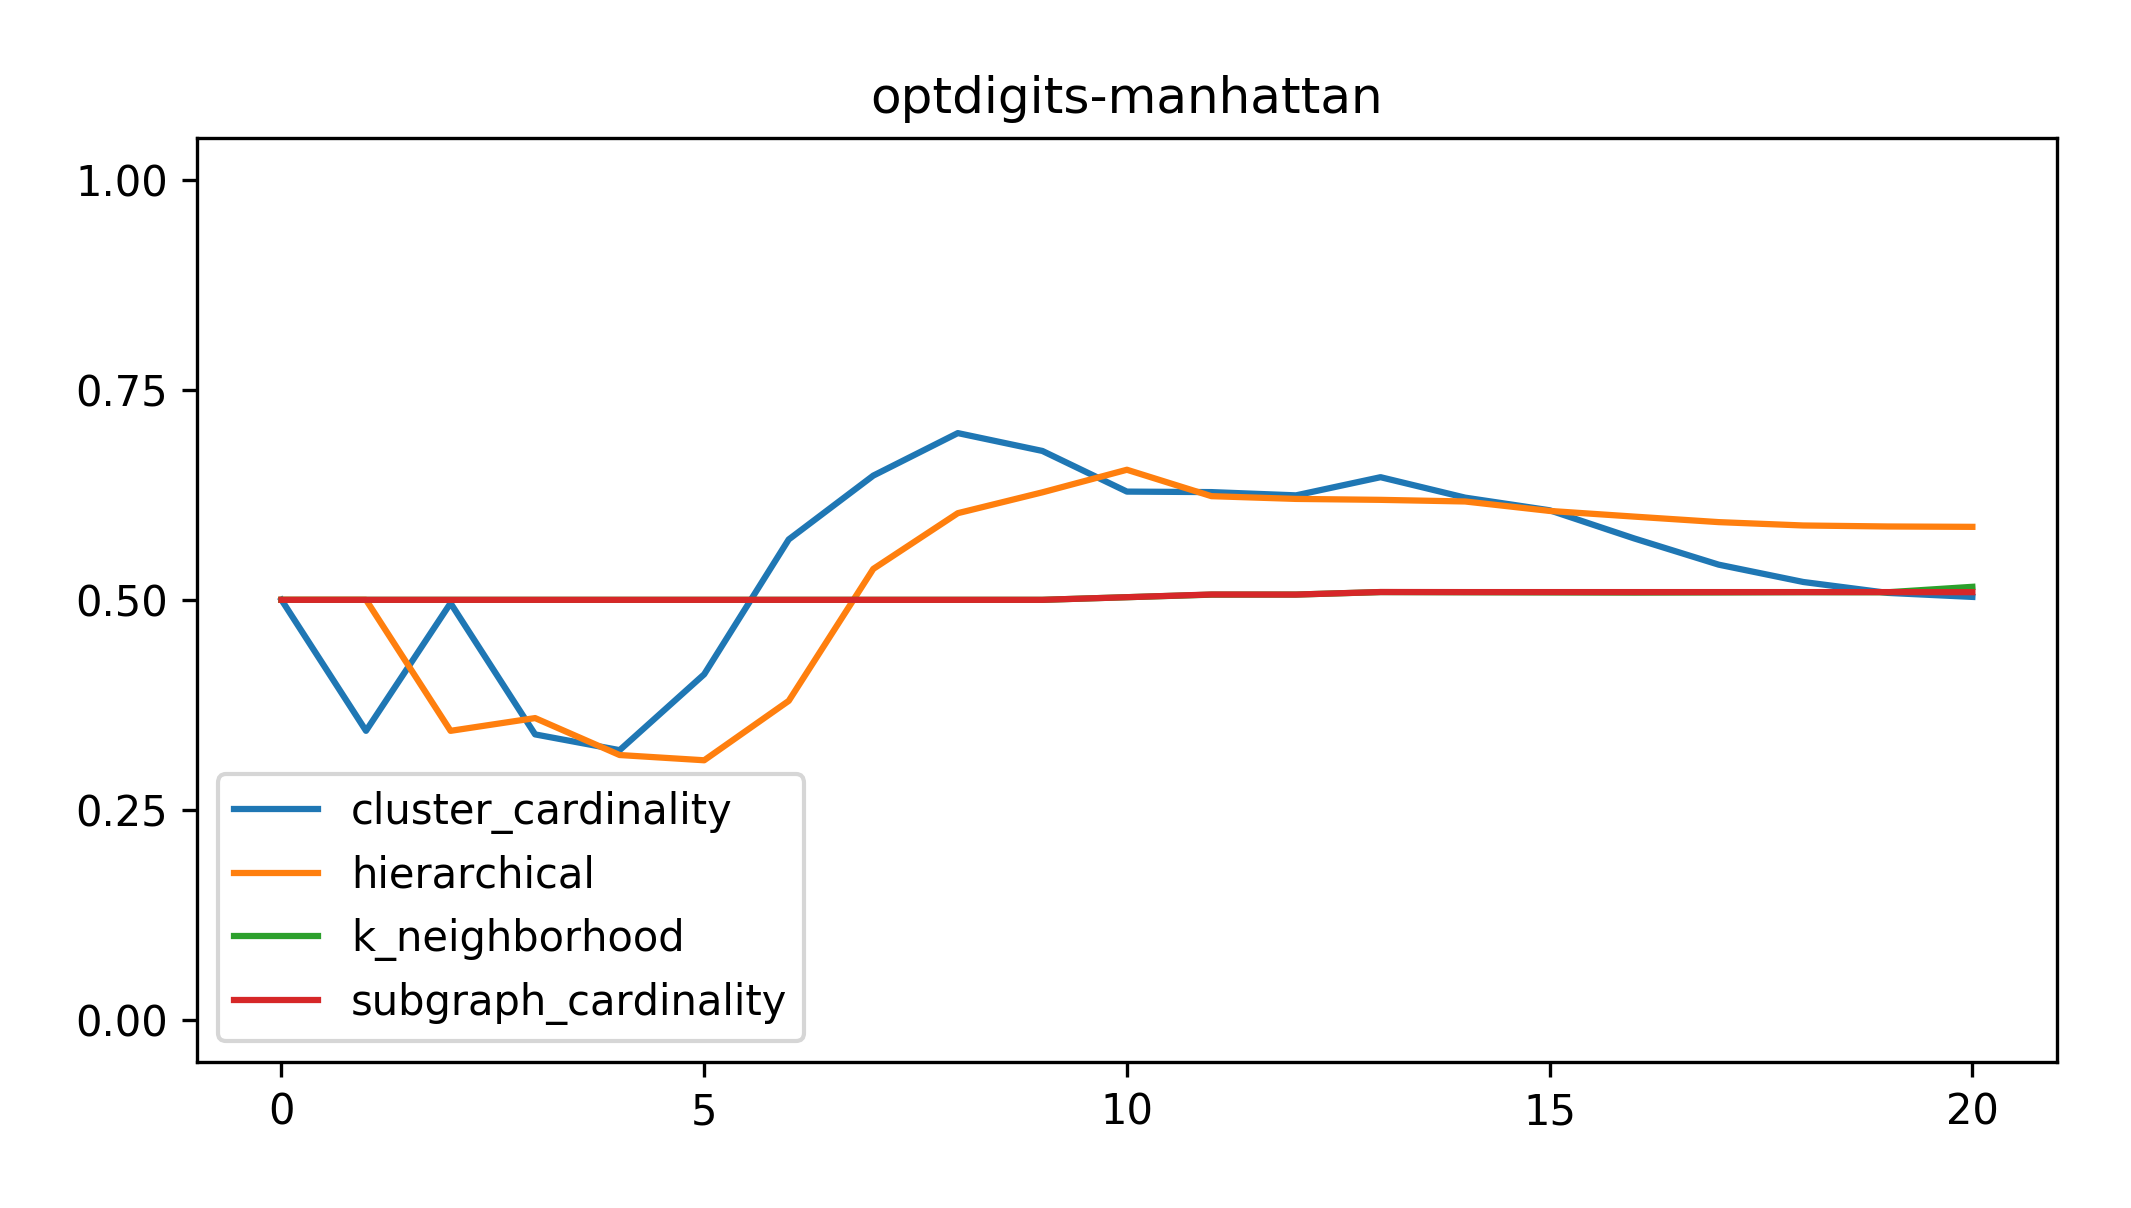
\includegraphics[width=2.2in]{kdd/static/auc_vs_depth/optdigits-manhattan.png}

% Pima
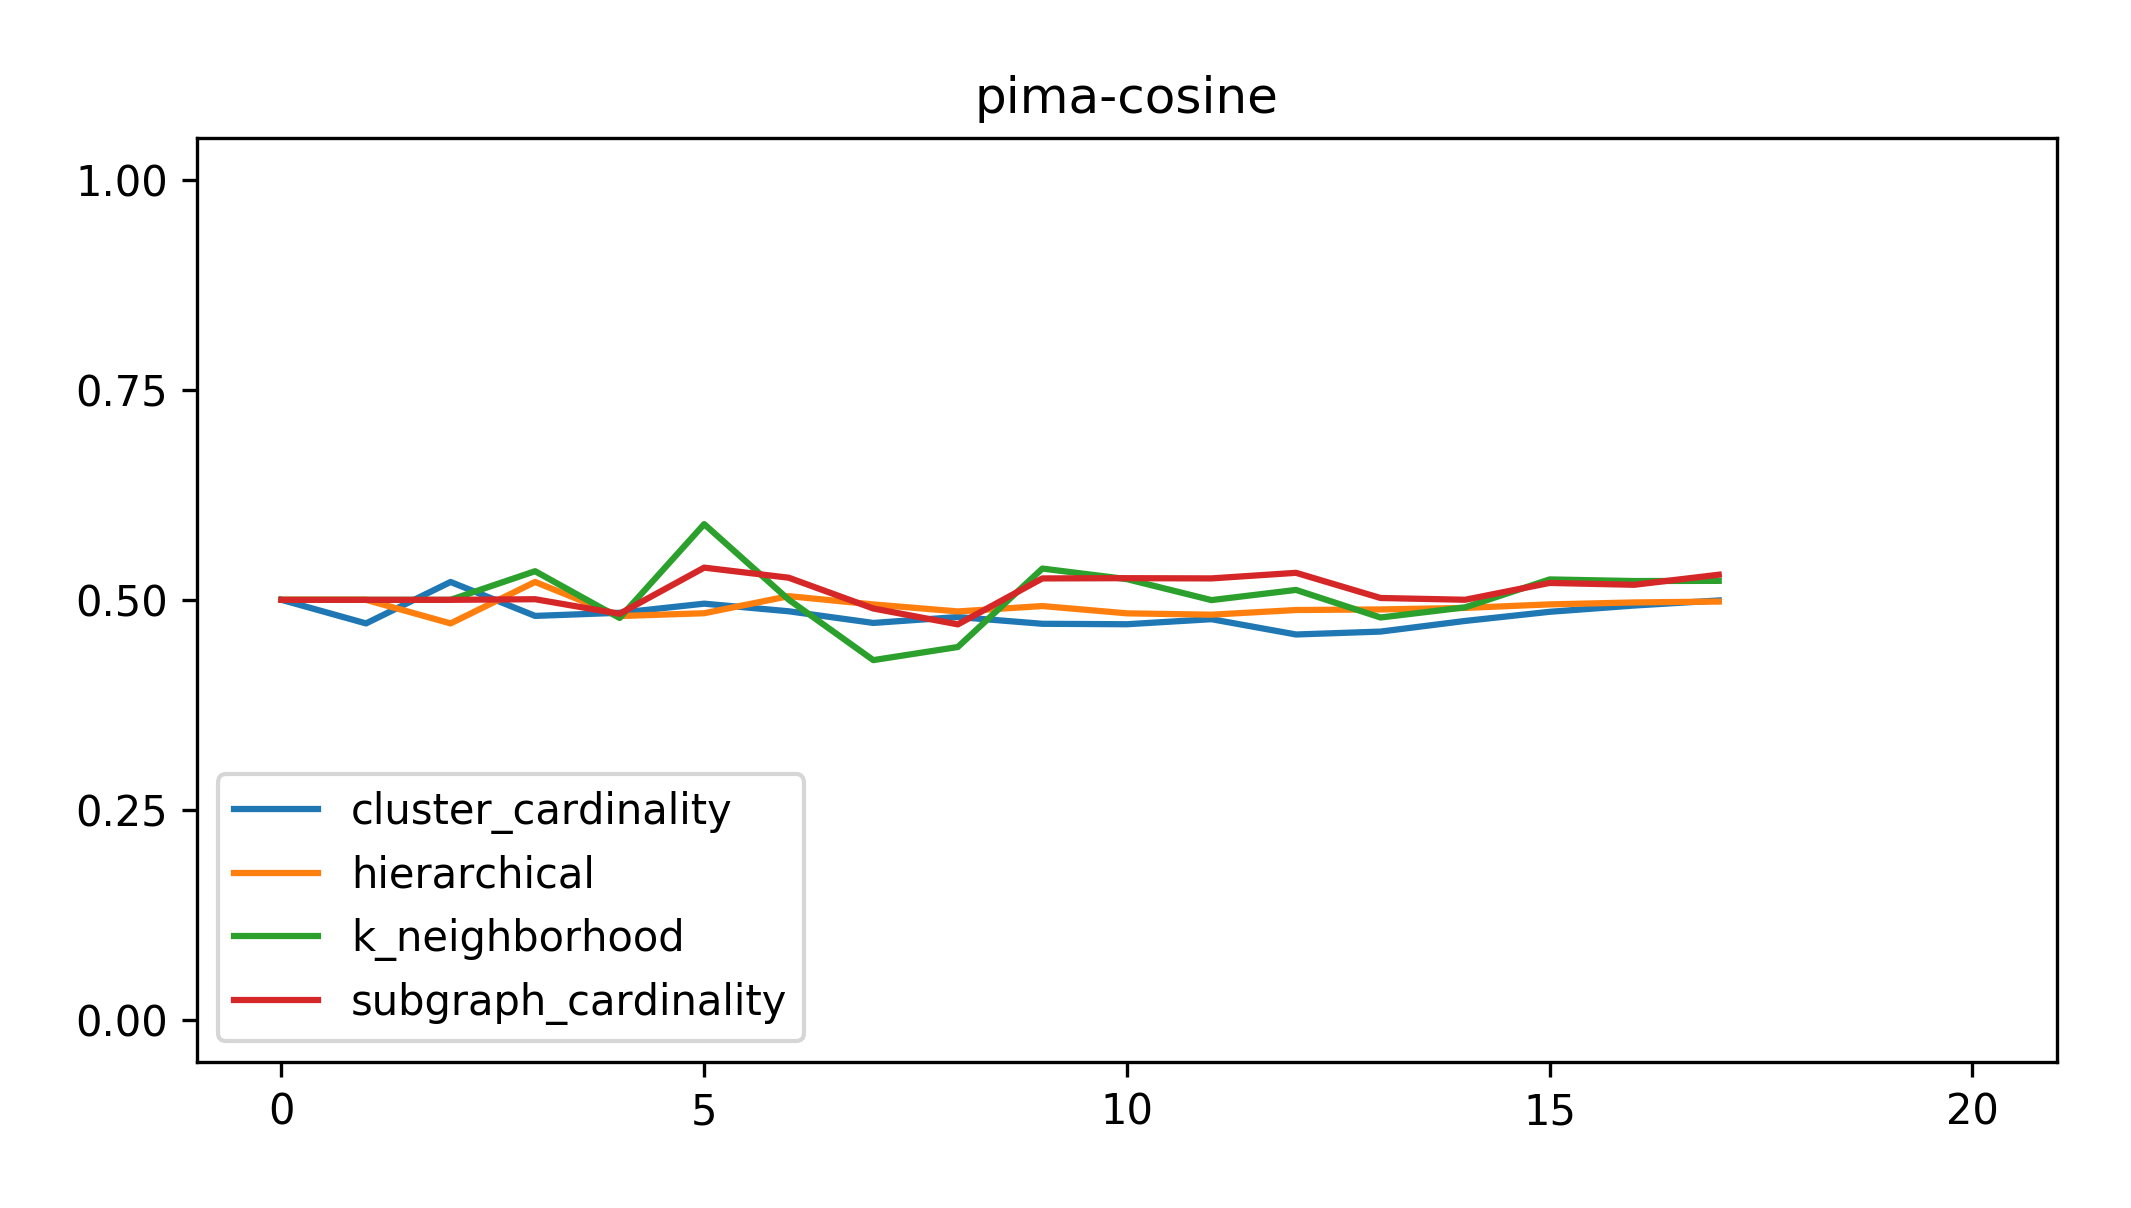
\includegraphics[width=2.2in]{kdd/static/auc_vs_depth/pima-cosine.png}
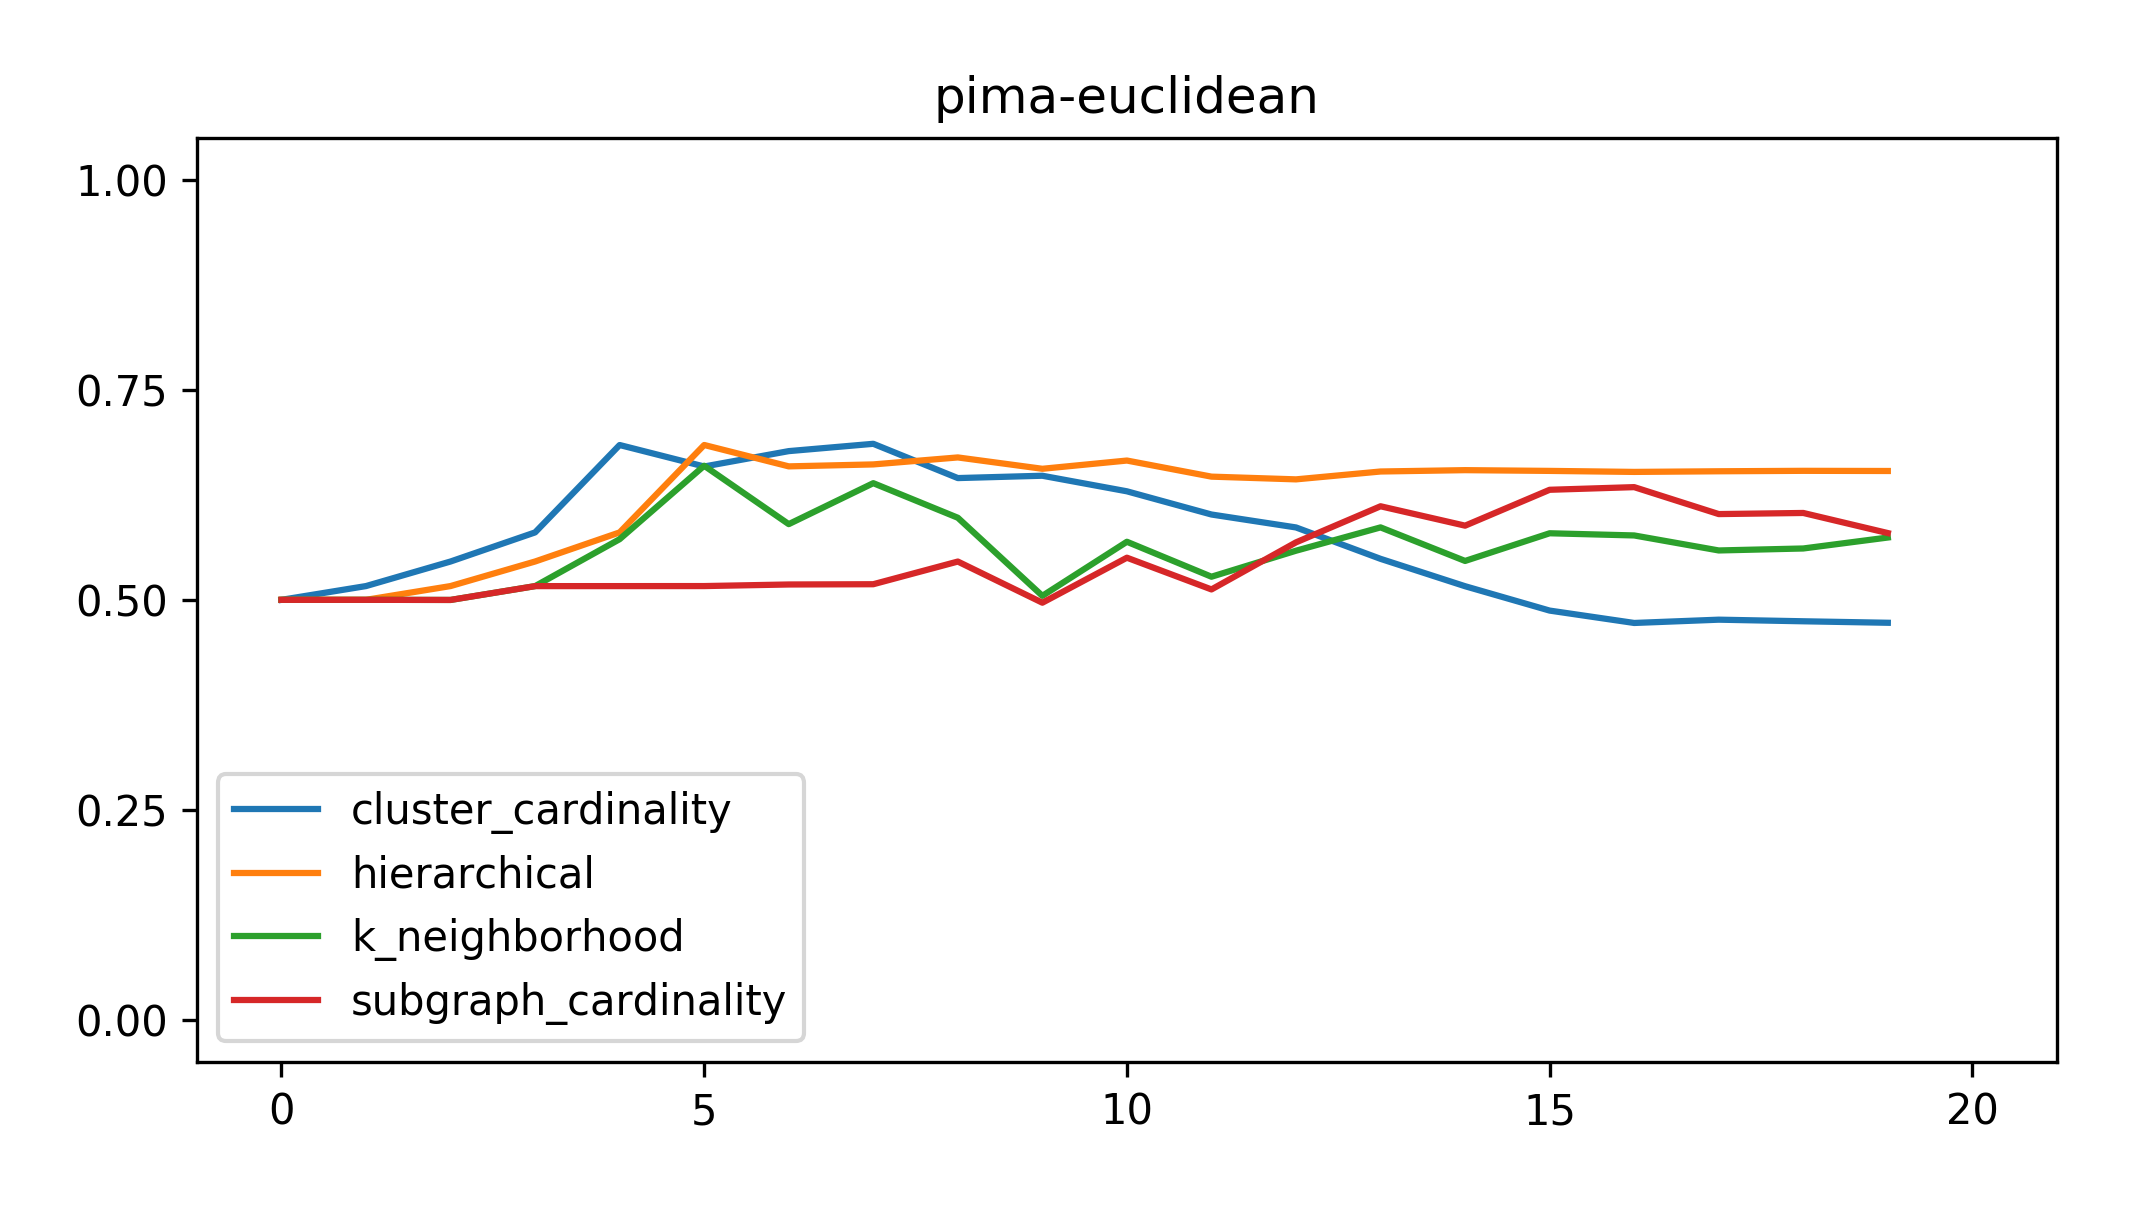
\includegraphics[width=2.2in]{kdd/static/auc_vs_depth/pima-euclidean.png}
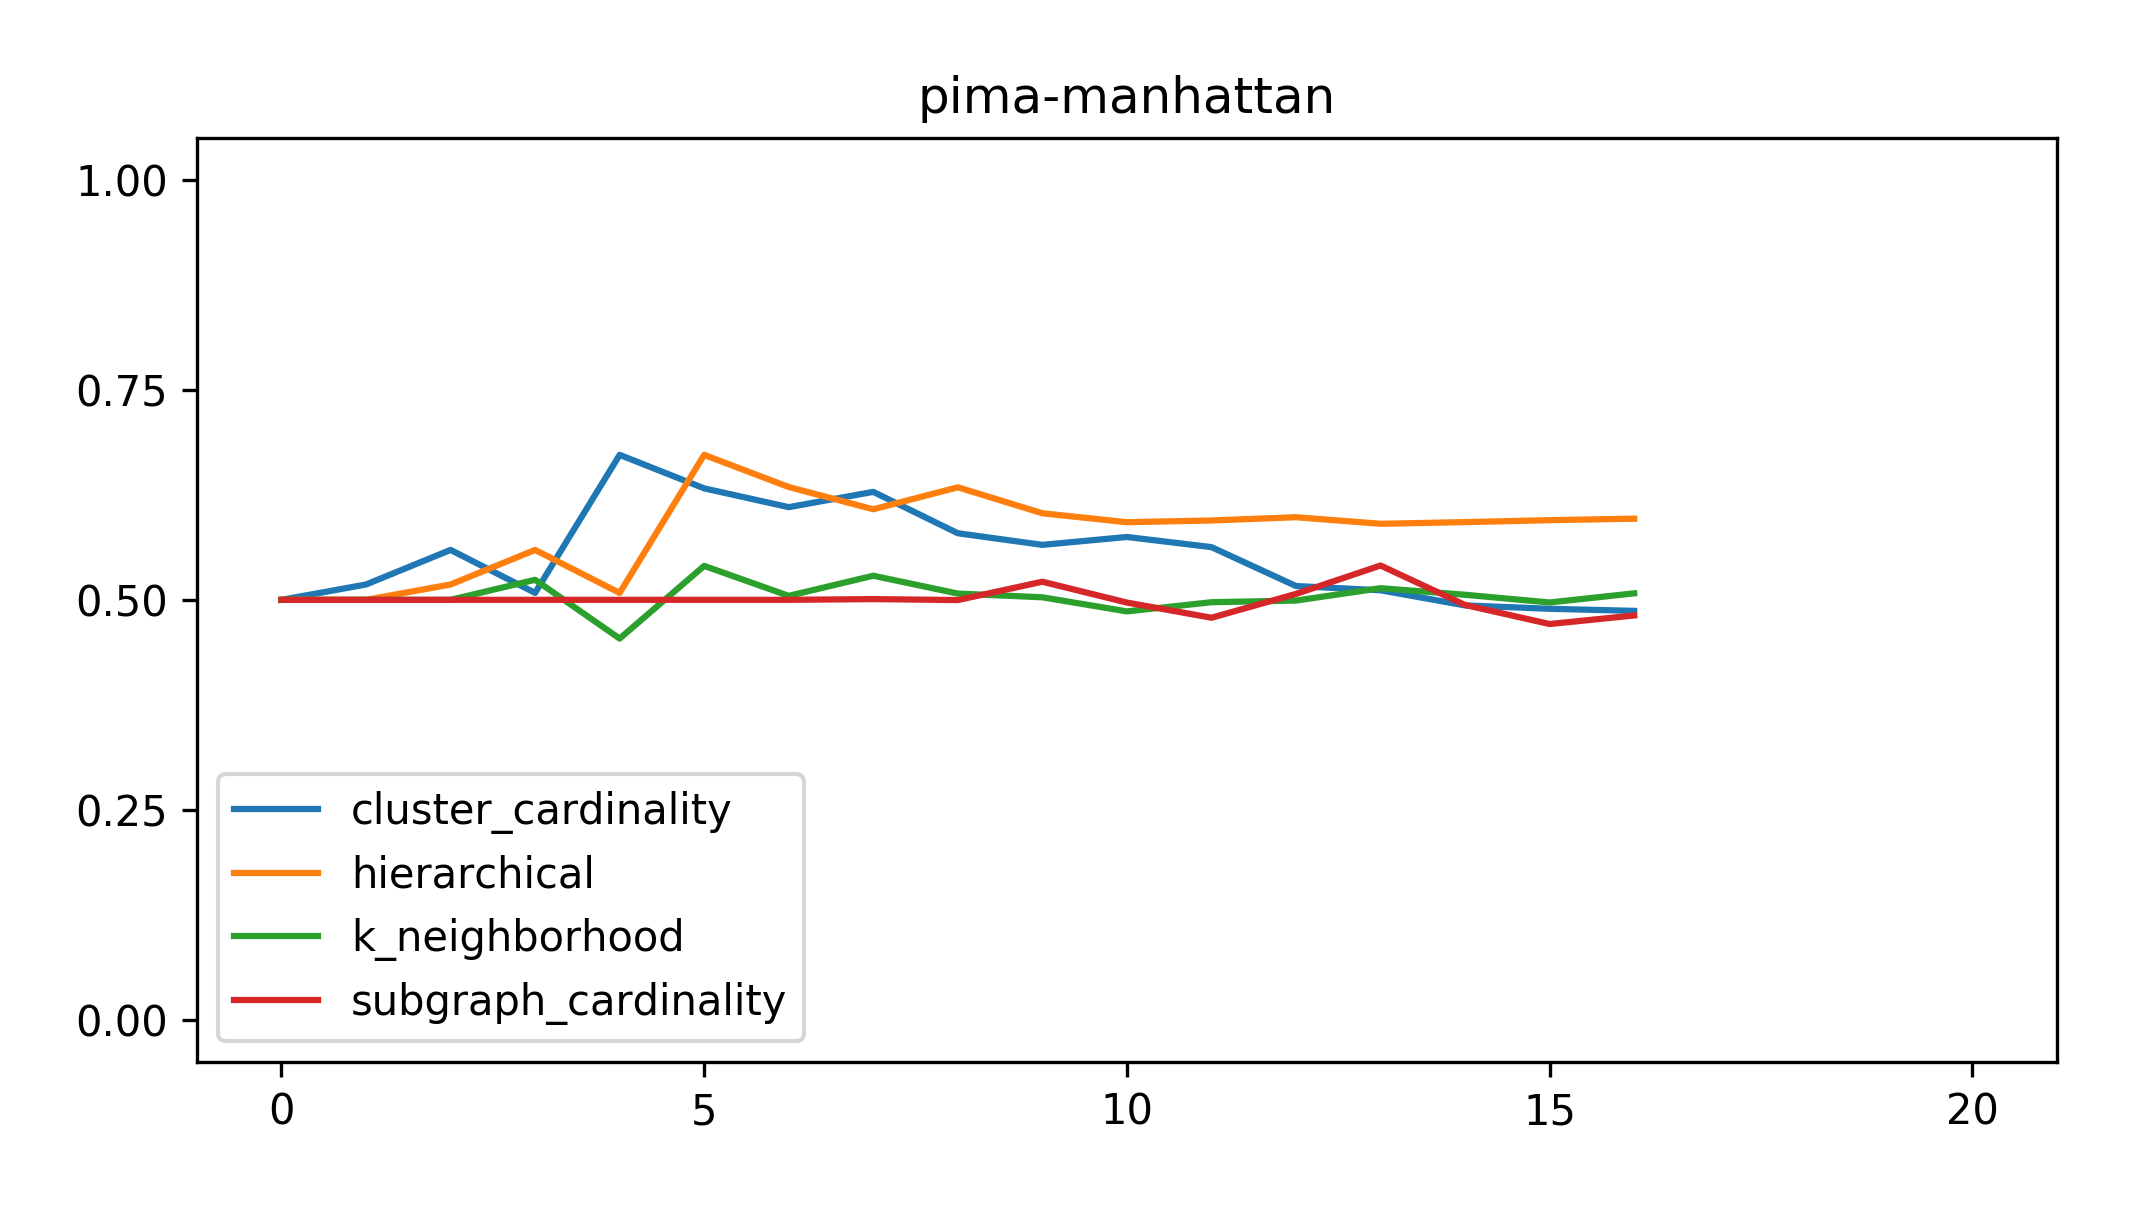
\includegraphics[width=2.2in]{kdd/static/auc_vs_depth/pima-manhattan.png}

% Satellite
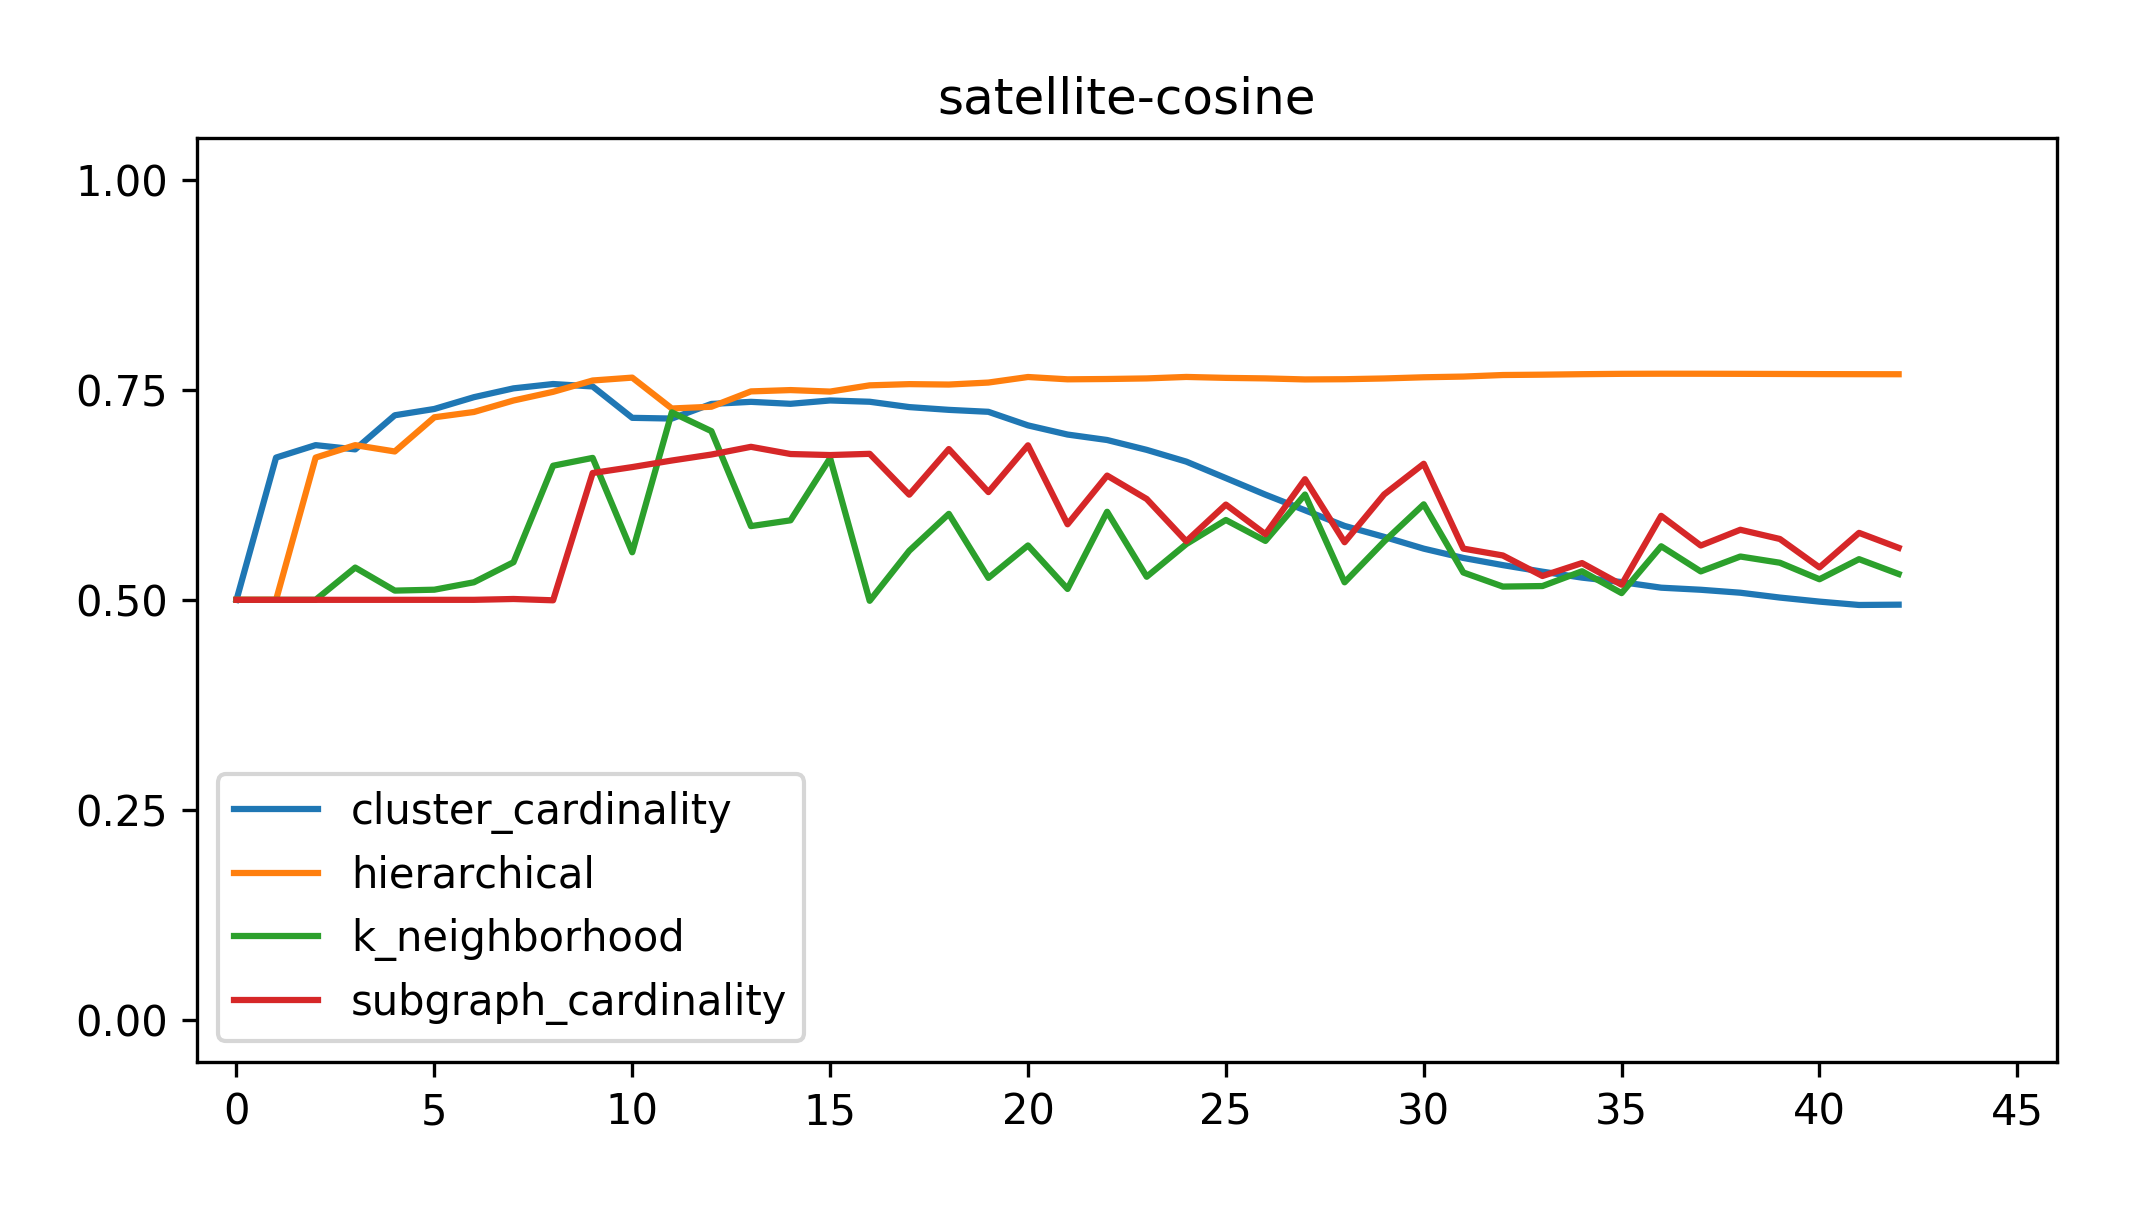
\includegraphics[width=2.2in]{kdd/static/auc_vs_depth/satellite-cosine.png}
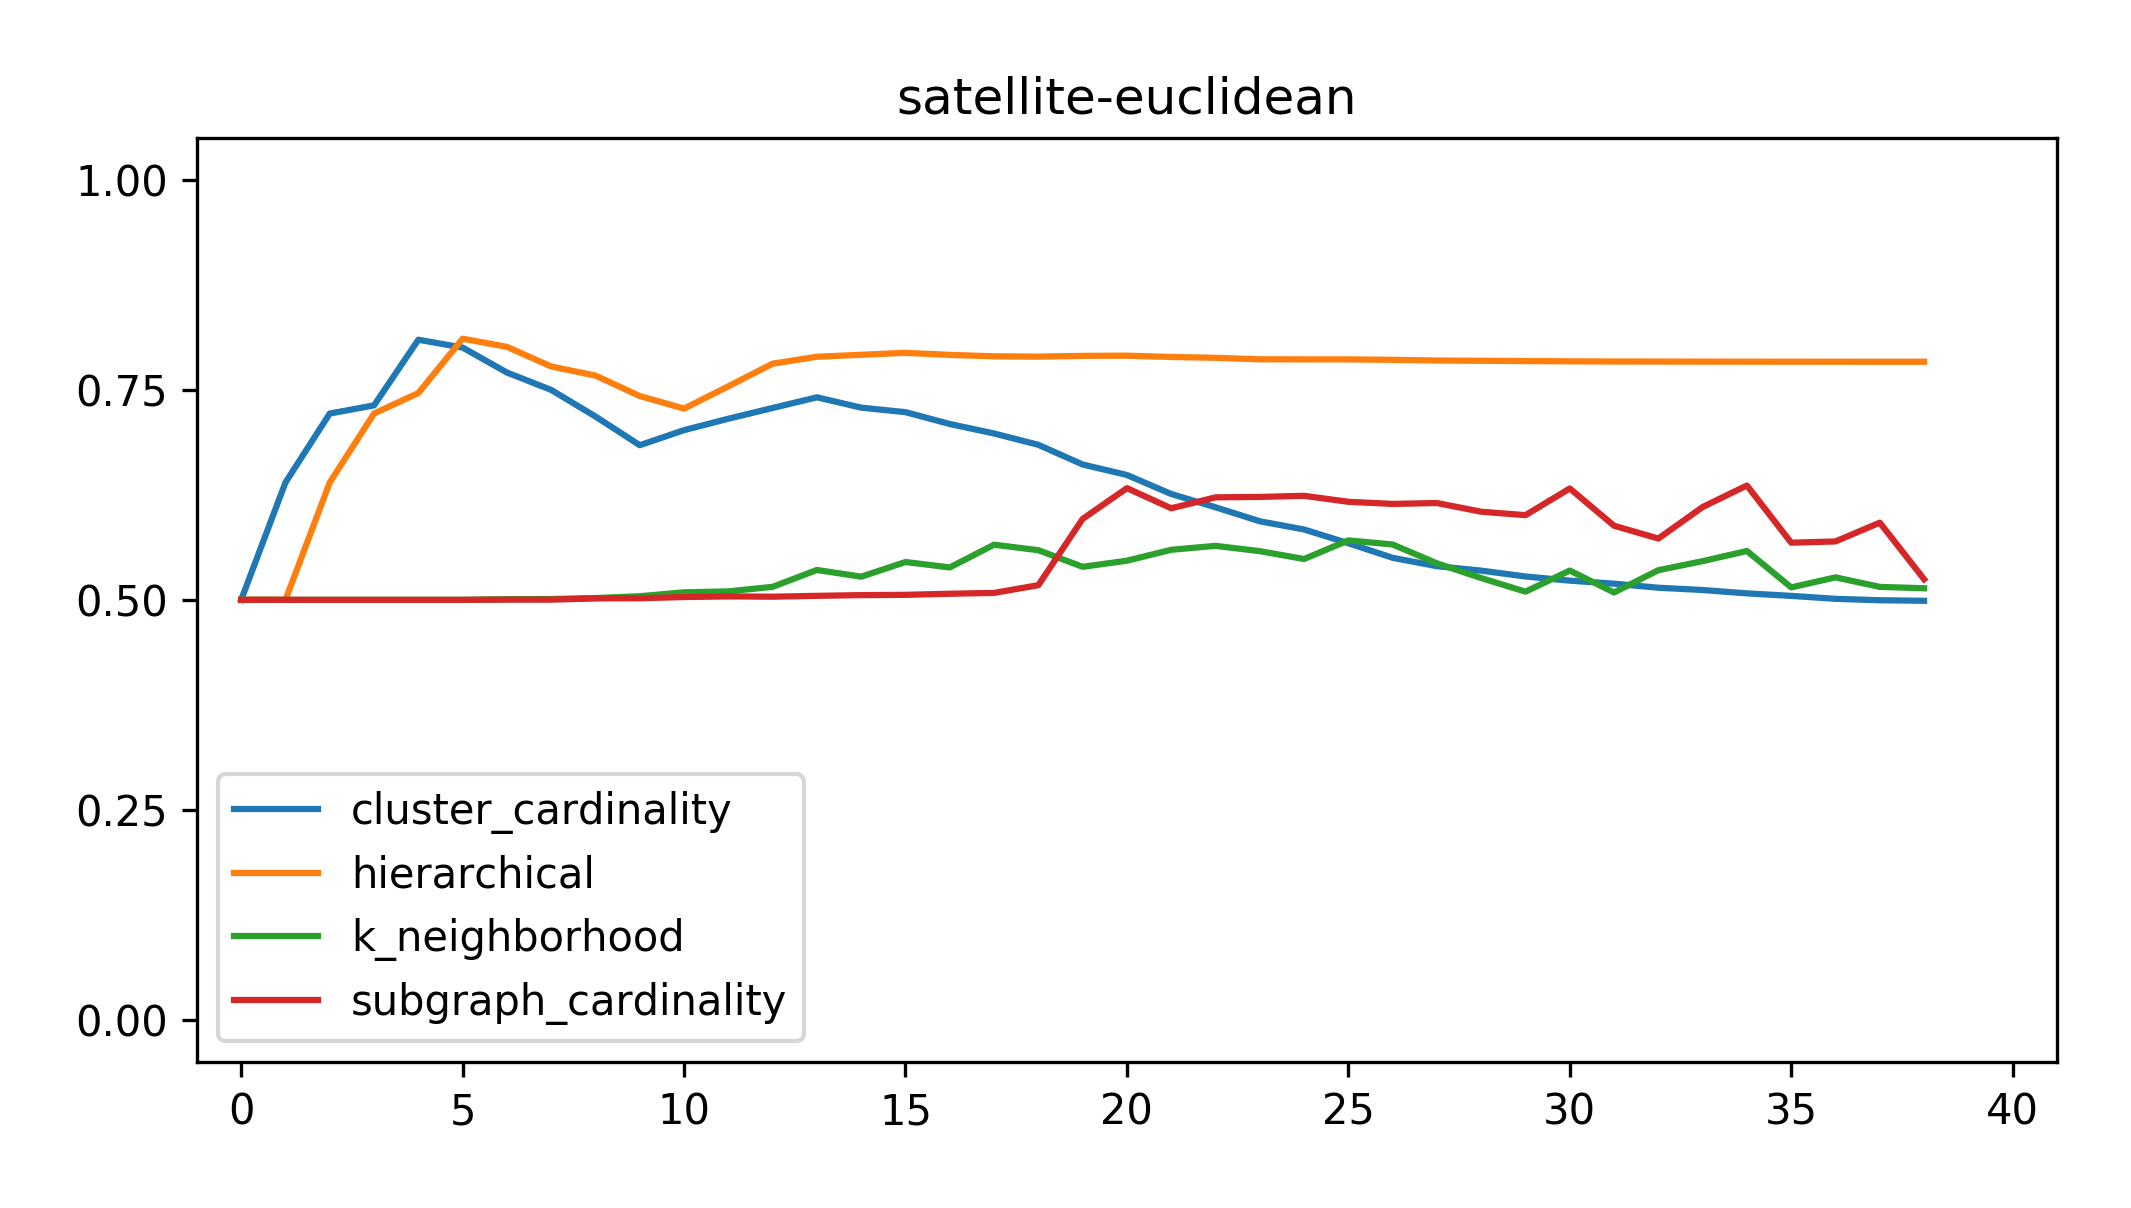
\includegraphics[width=2.2in]{kdd/static/auc_vs_depth/satellite-euclidean.png}
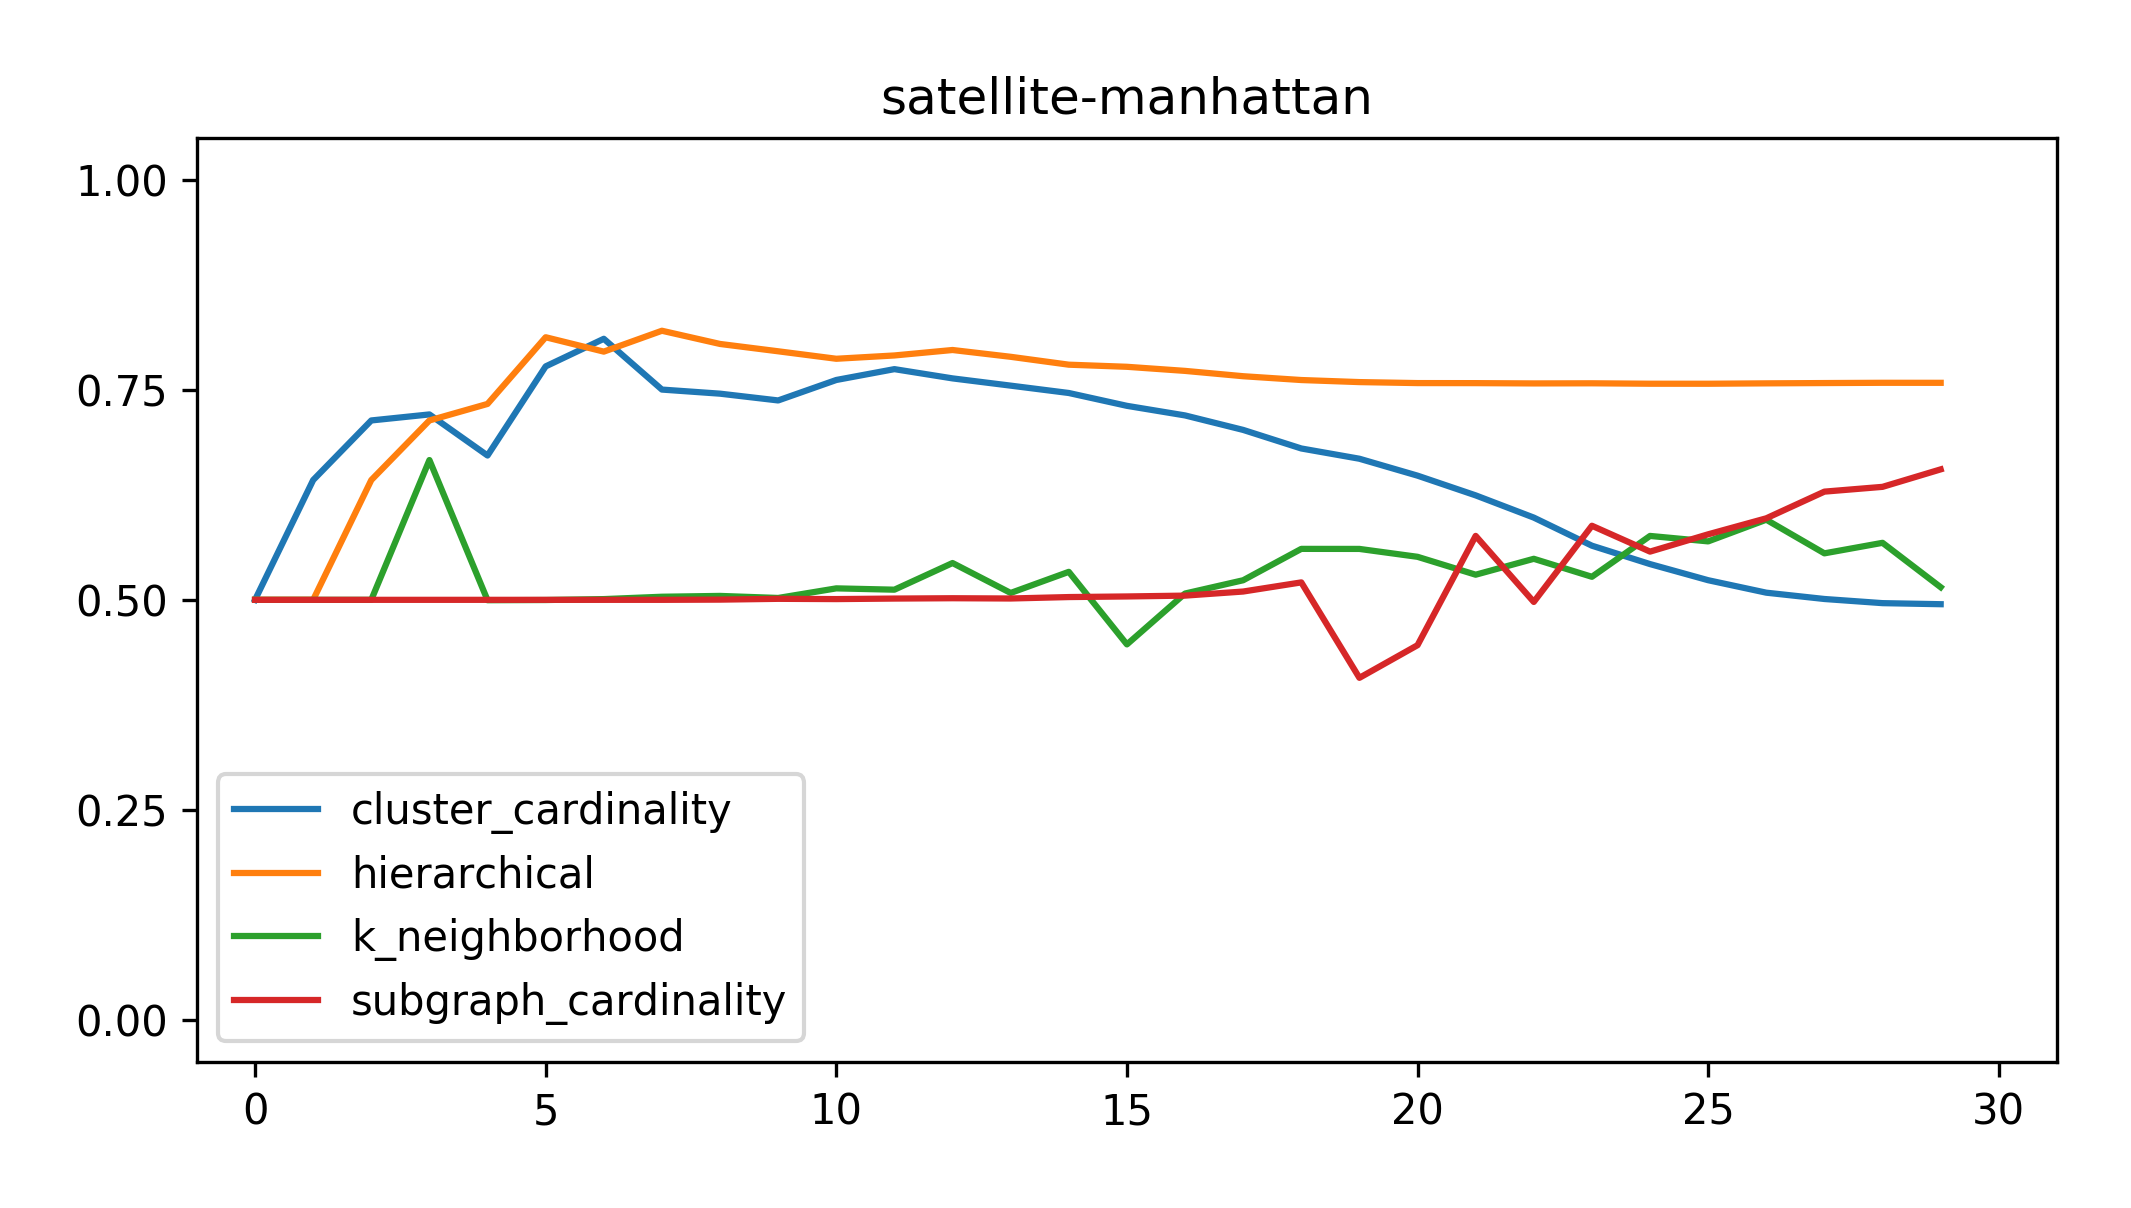
\includegraphics[width=2.2in]{kdd/static/auc_vs_depth/satellite-manhattan.png}

\caption{
Plots of ROC-AUC vs Depth for our measures of Anomolousness.
}

\label{results:datasets_2}
\end{figure*}

\begin{figure*}[!t]
\centering
% Satimage-2
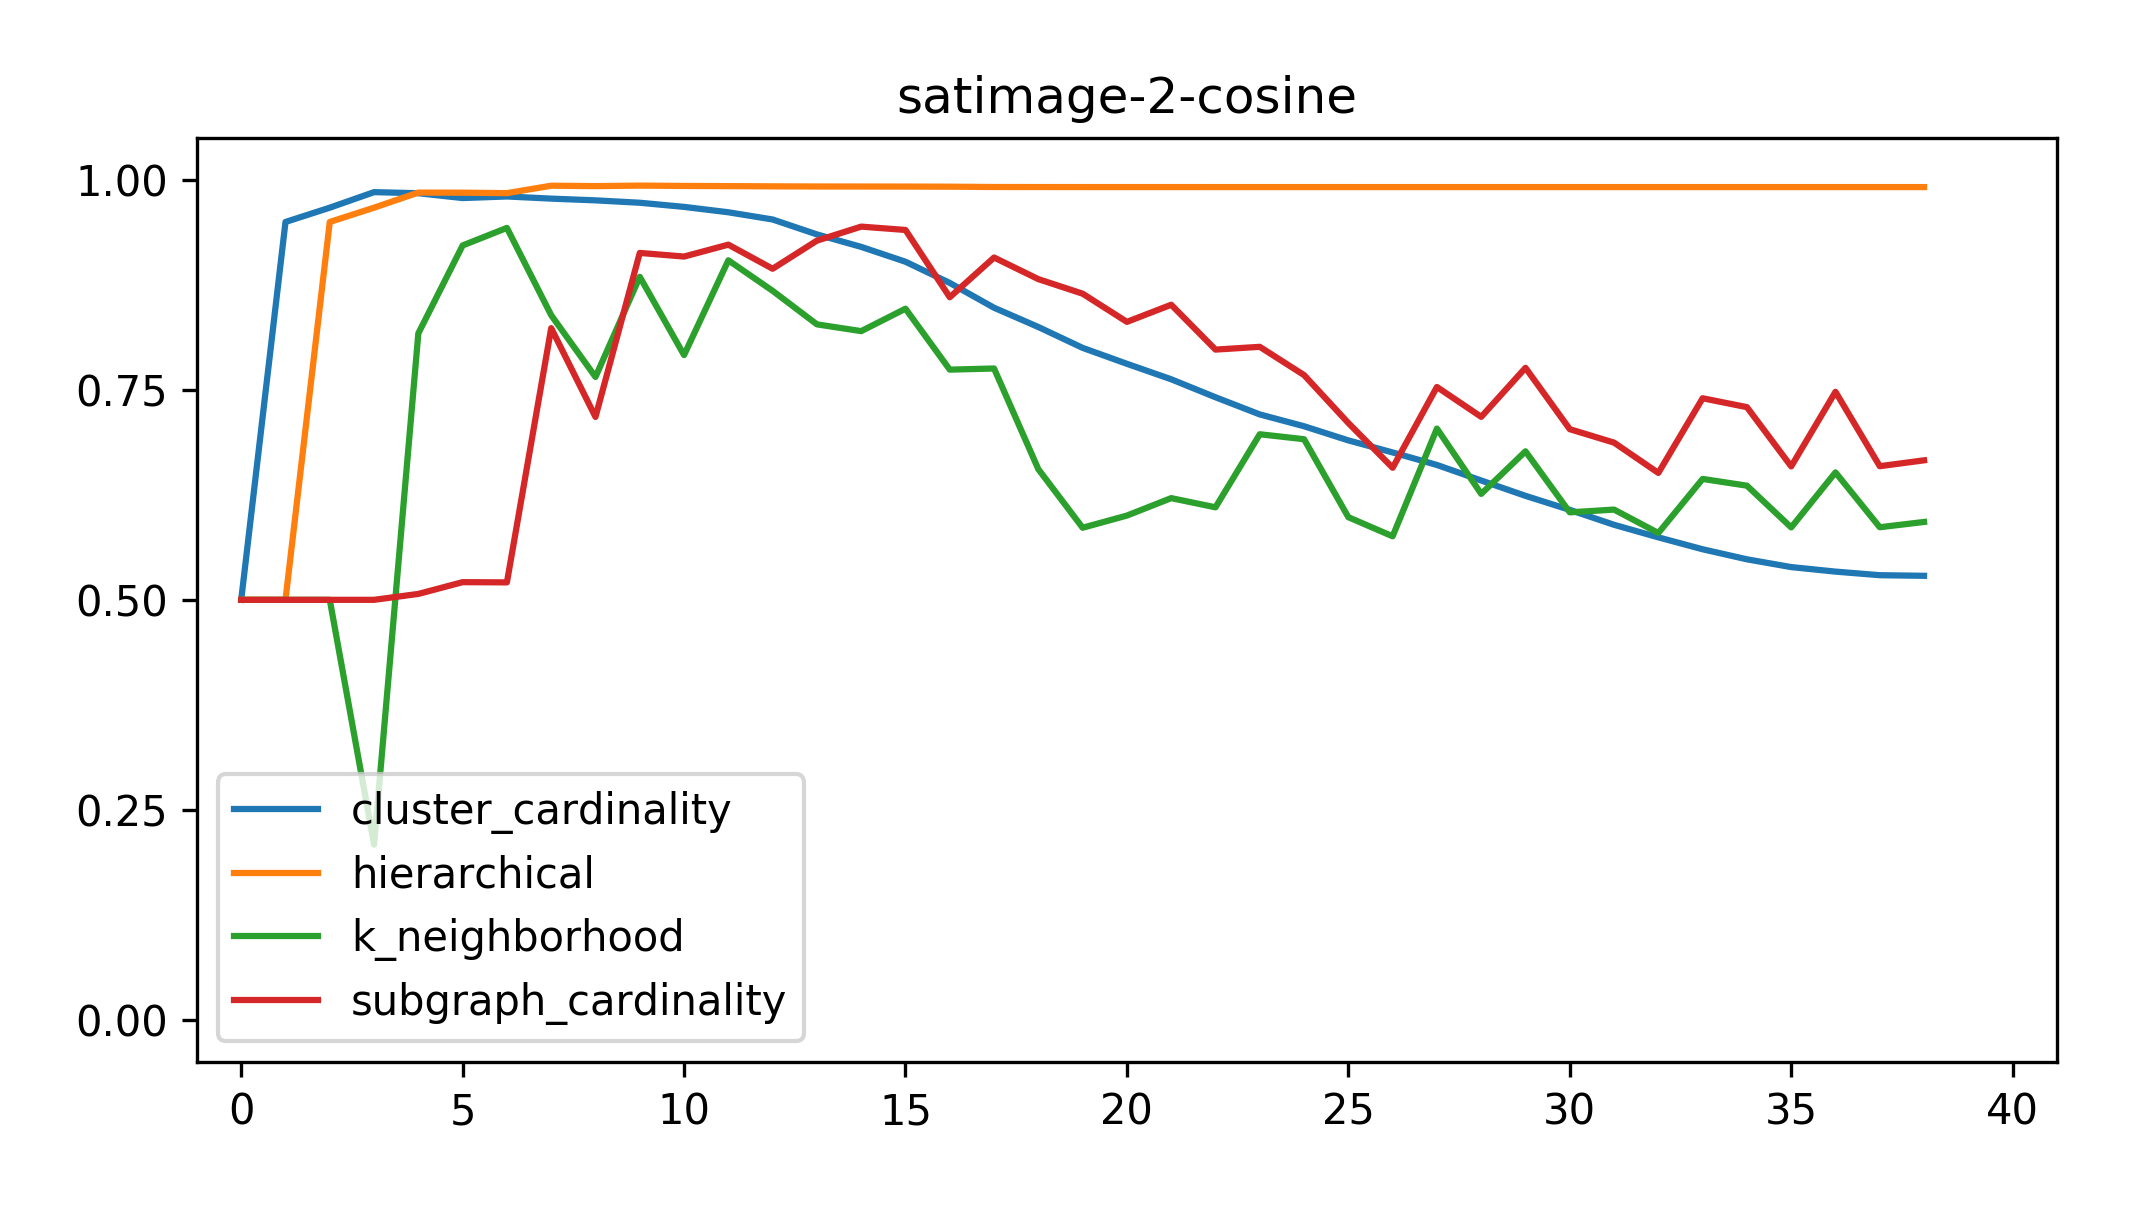
\includegraphics[width=2.2in]{kdd/static/auc_vs_depth/satimage-2-cosine.png}
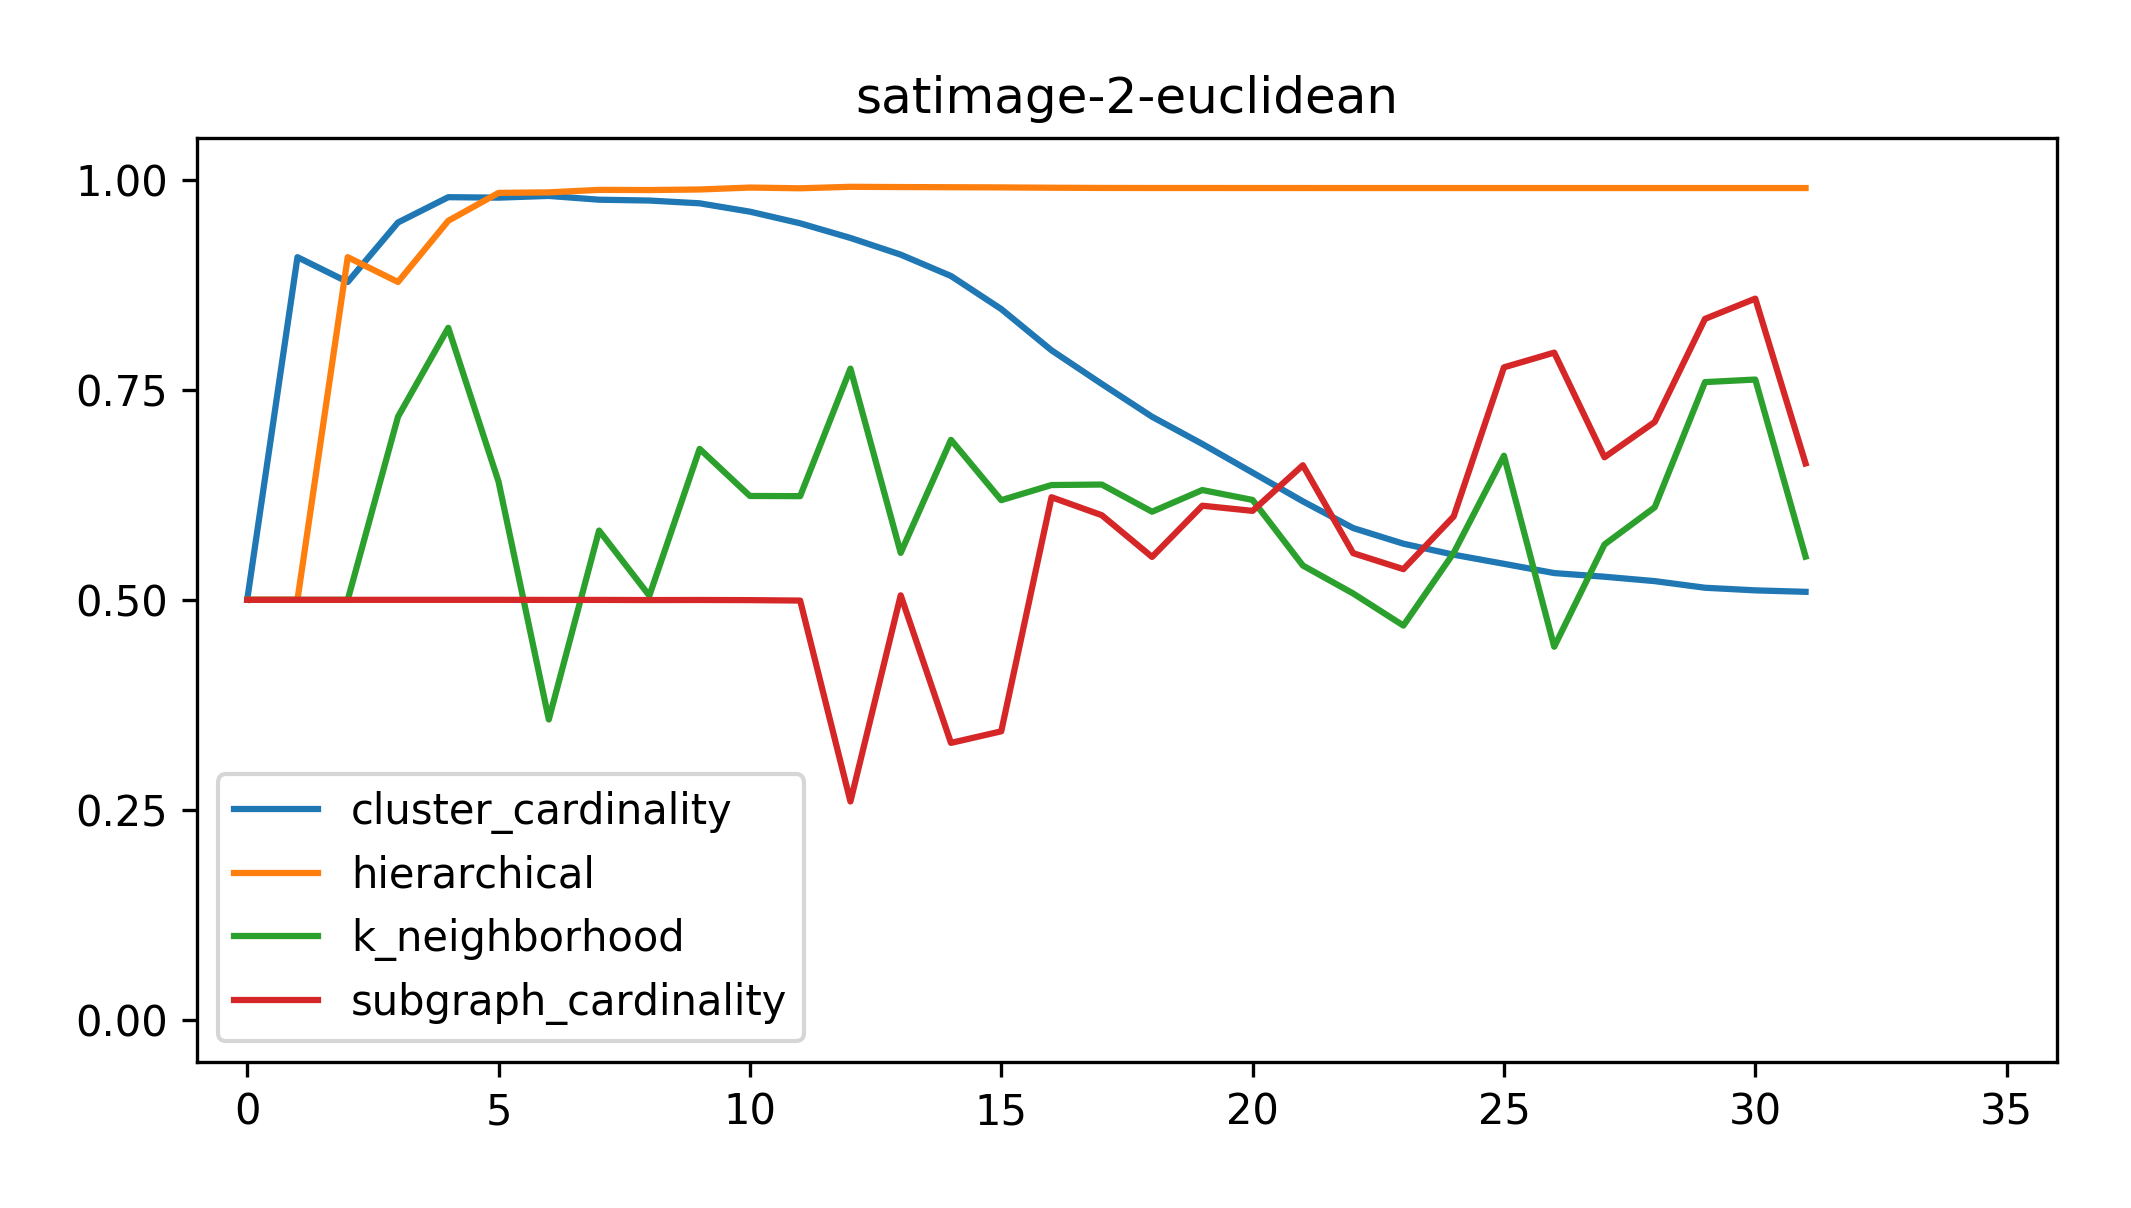
\includegraphics[width=2.2in]{kdd/static/auc_vs_depth/satimage-2-euclidean.png}
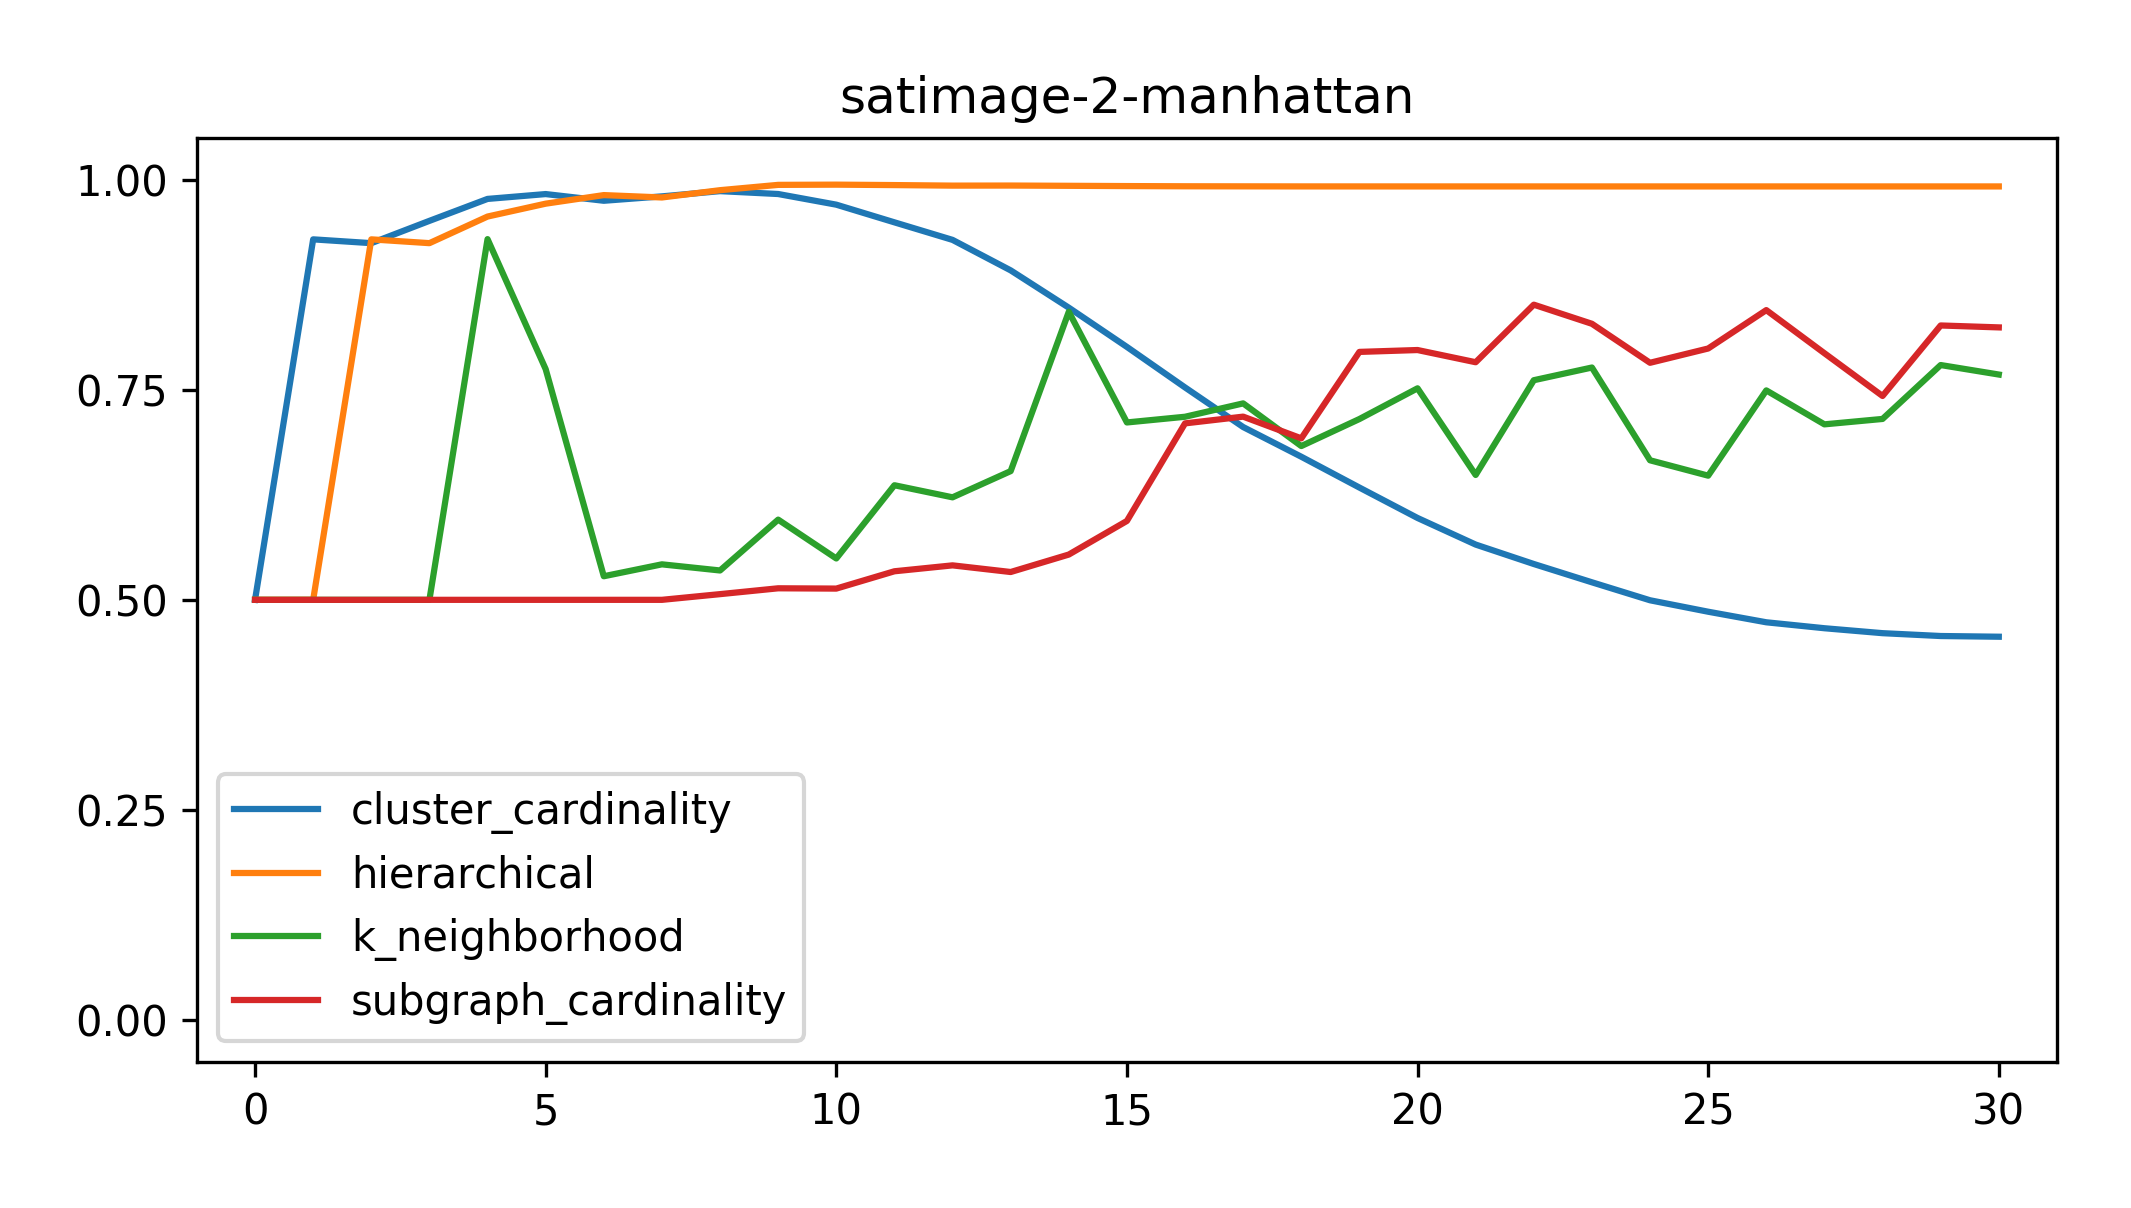
\includegraphics[width=2.2in]{kdd/static/auc_vs_depth/satimage-2-manhattan.png}

% Thyroid
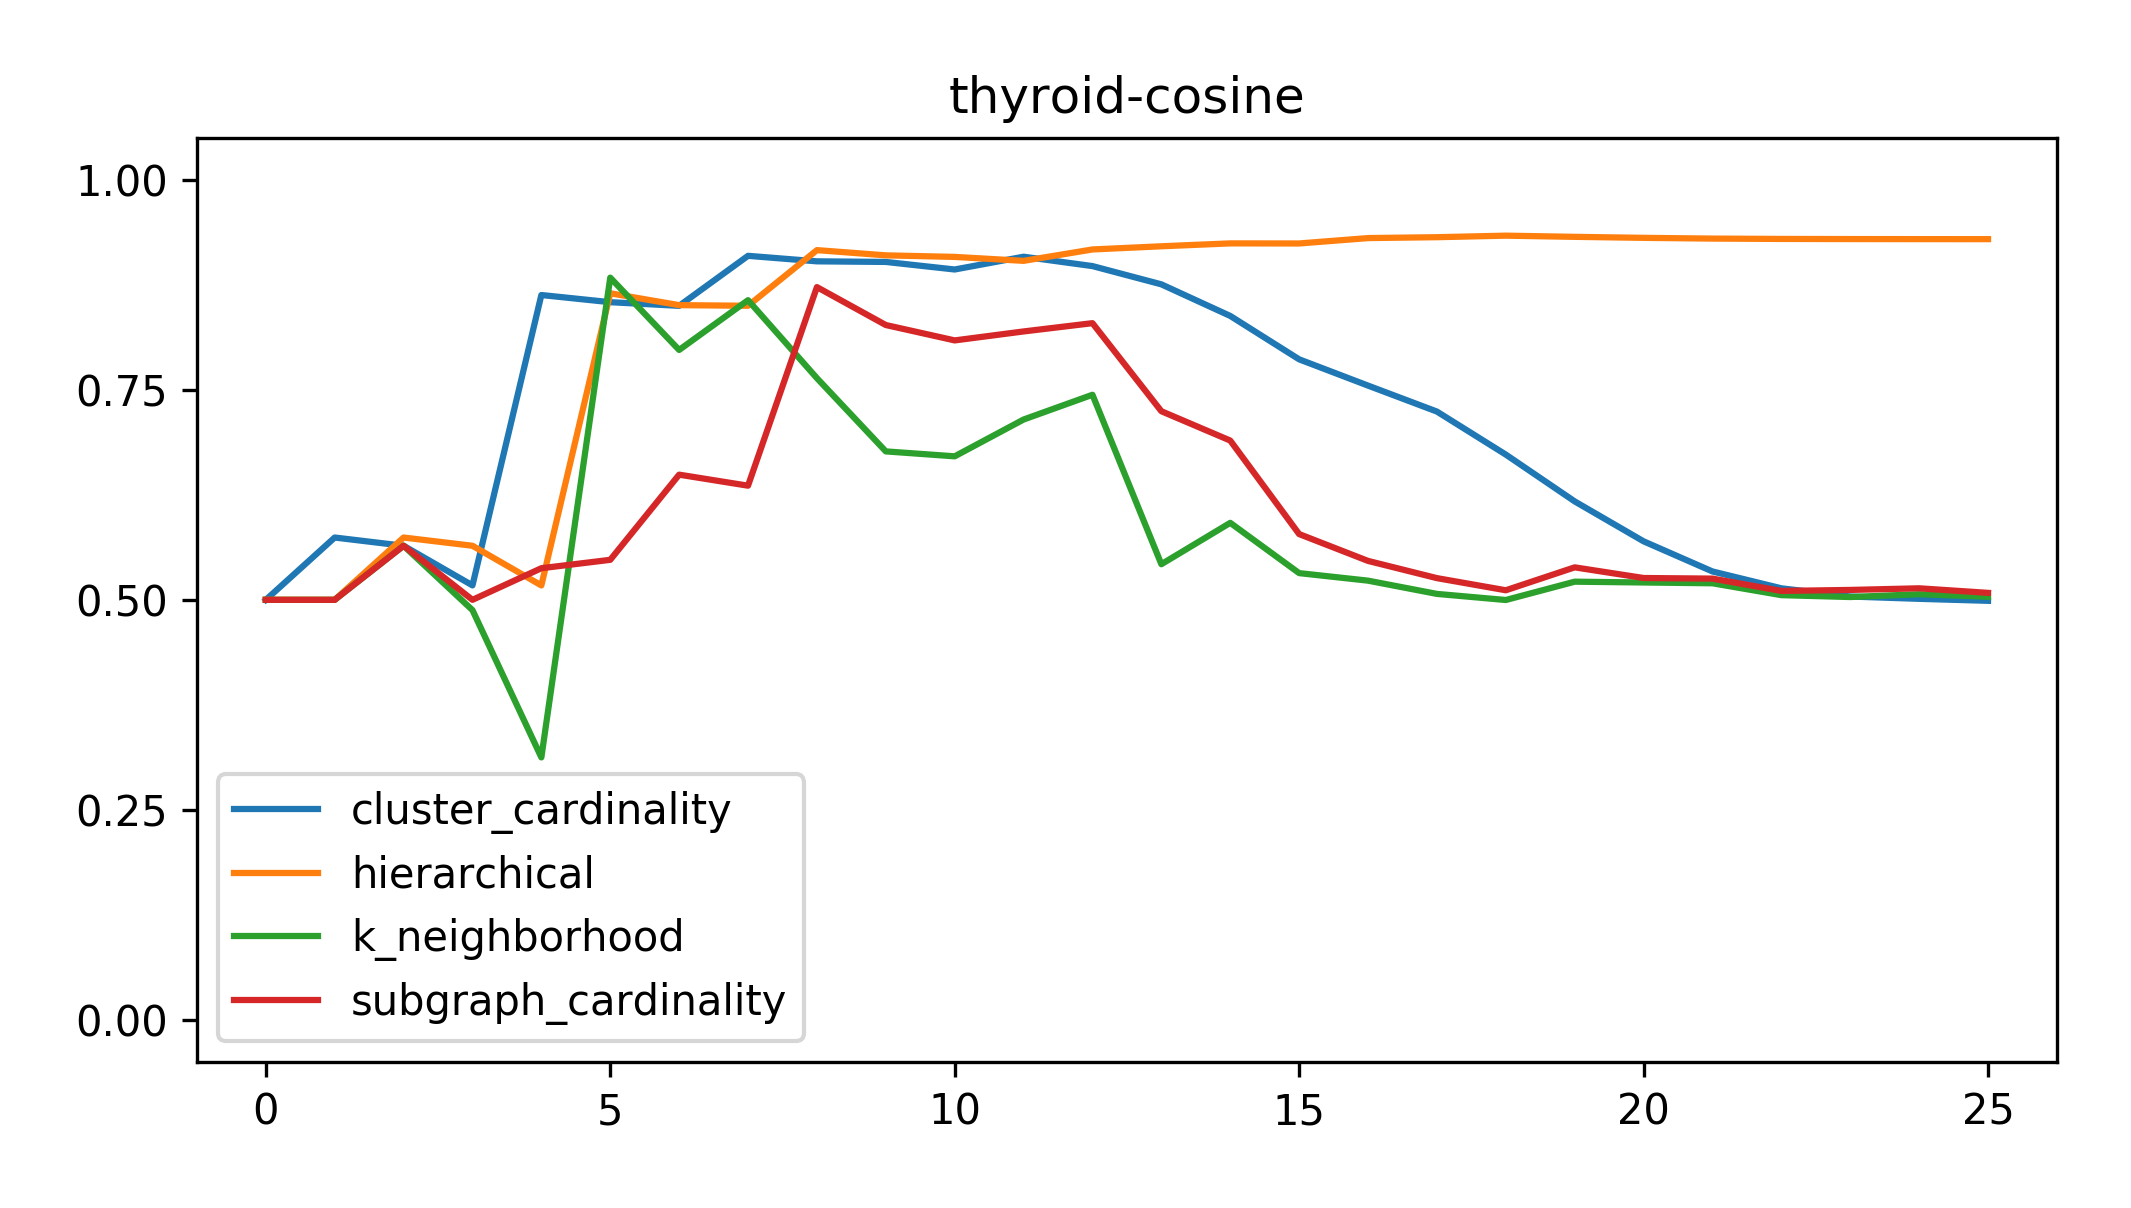
\includegraphics[width=2.2in]{kdd/static/auc_vs_depth/thyroid-cosine.png}
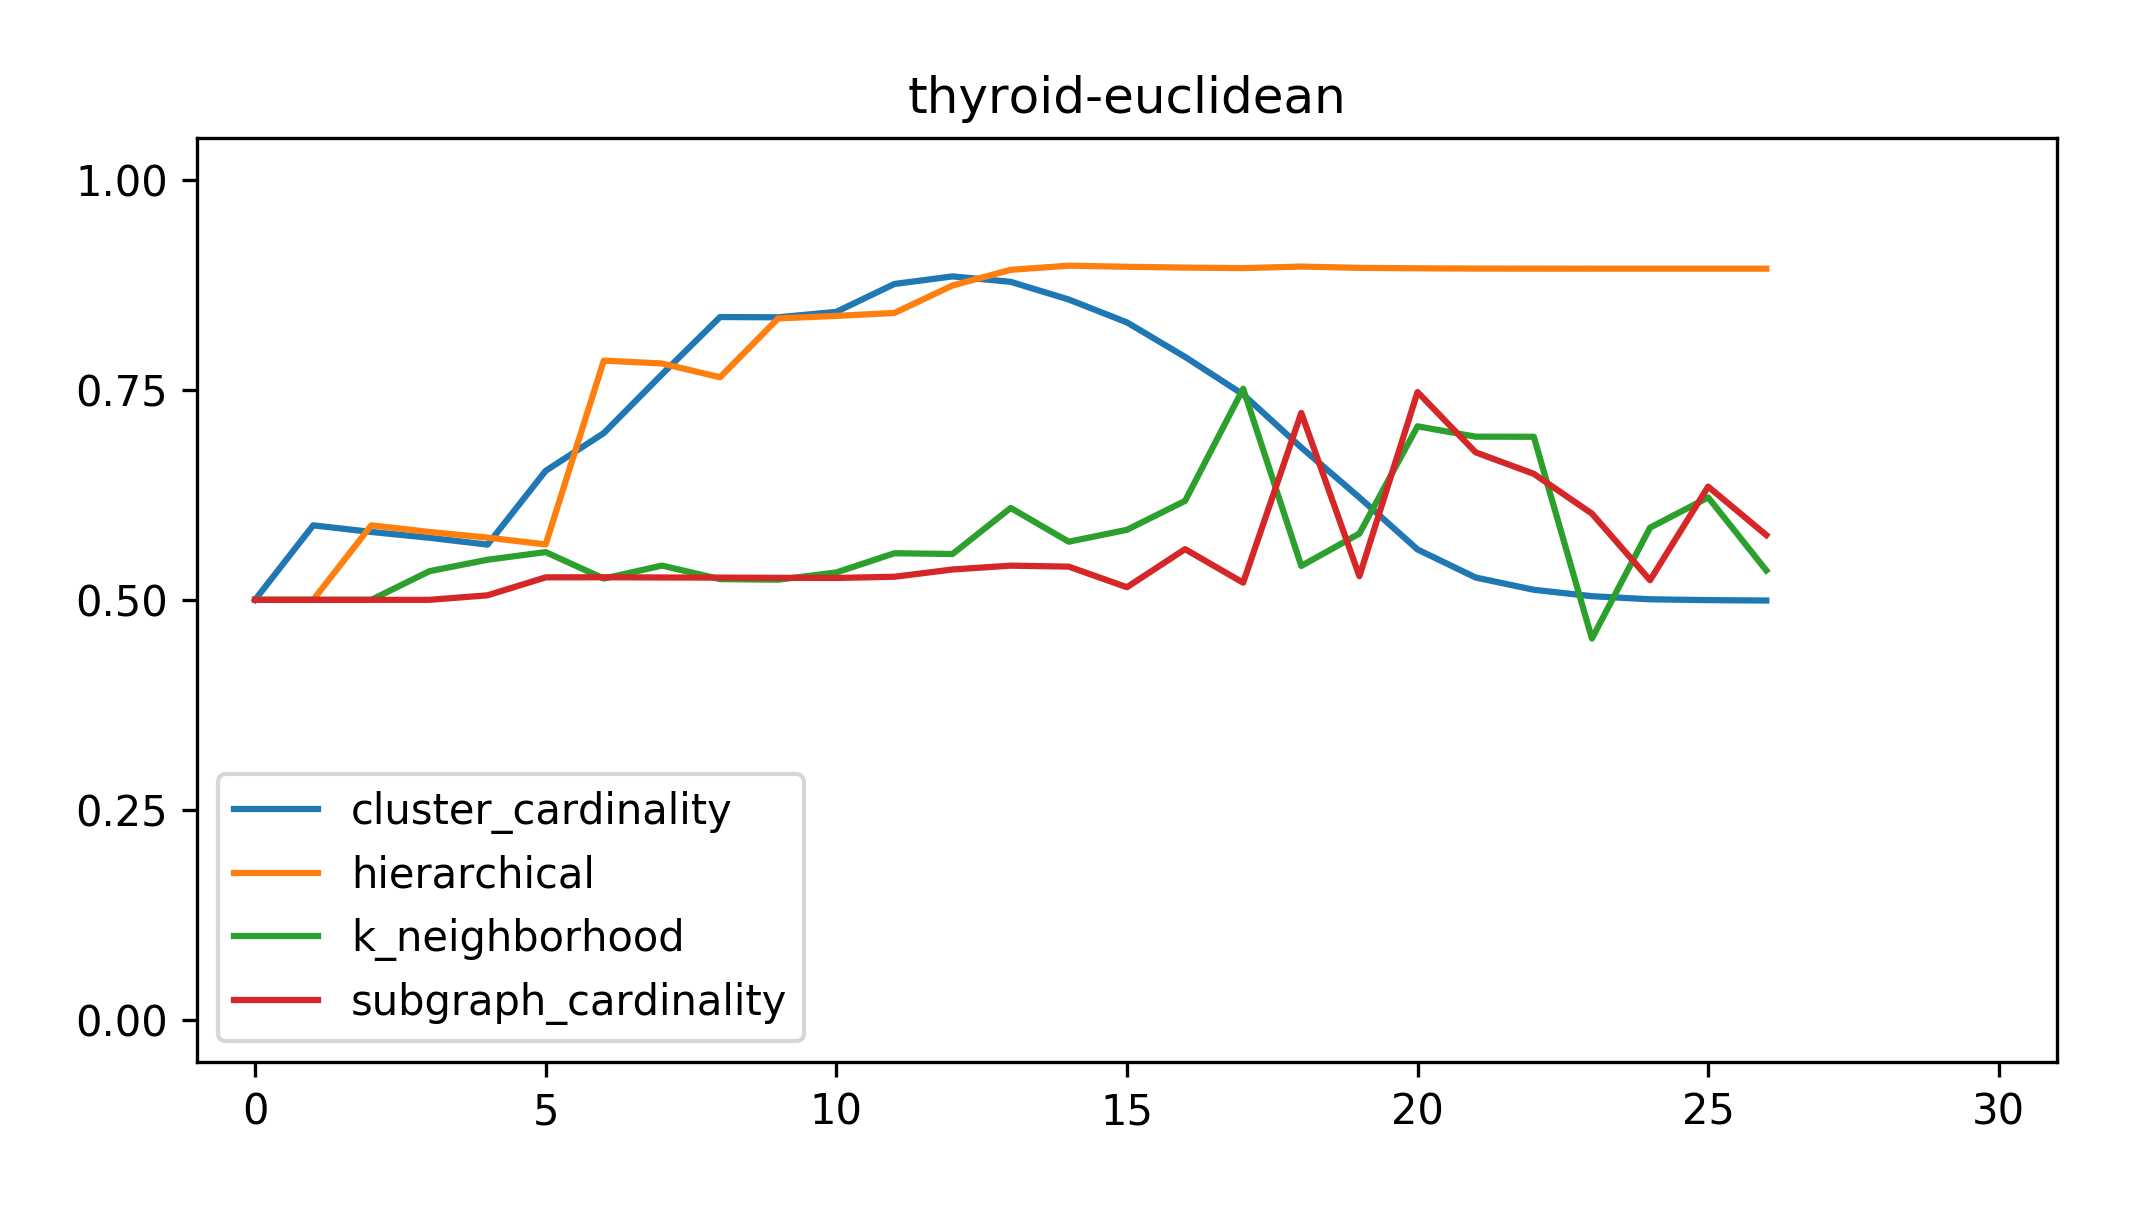
\includegraphics[width=2.2in]{kdd/static/auc_vs_depth/thyroid-euclidean.png}
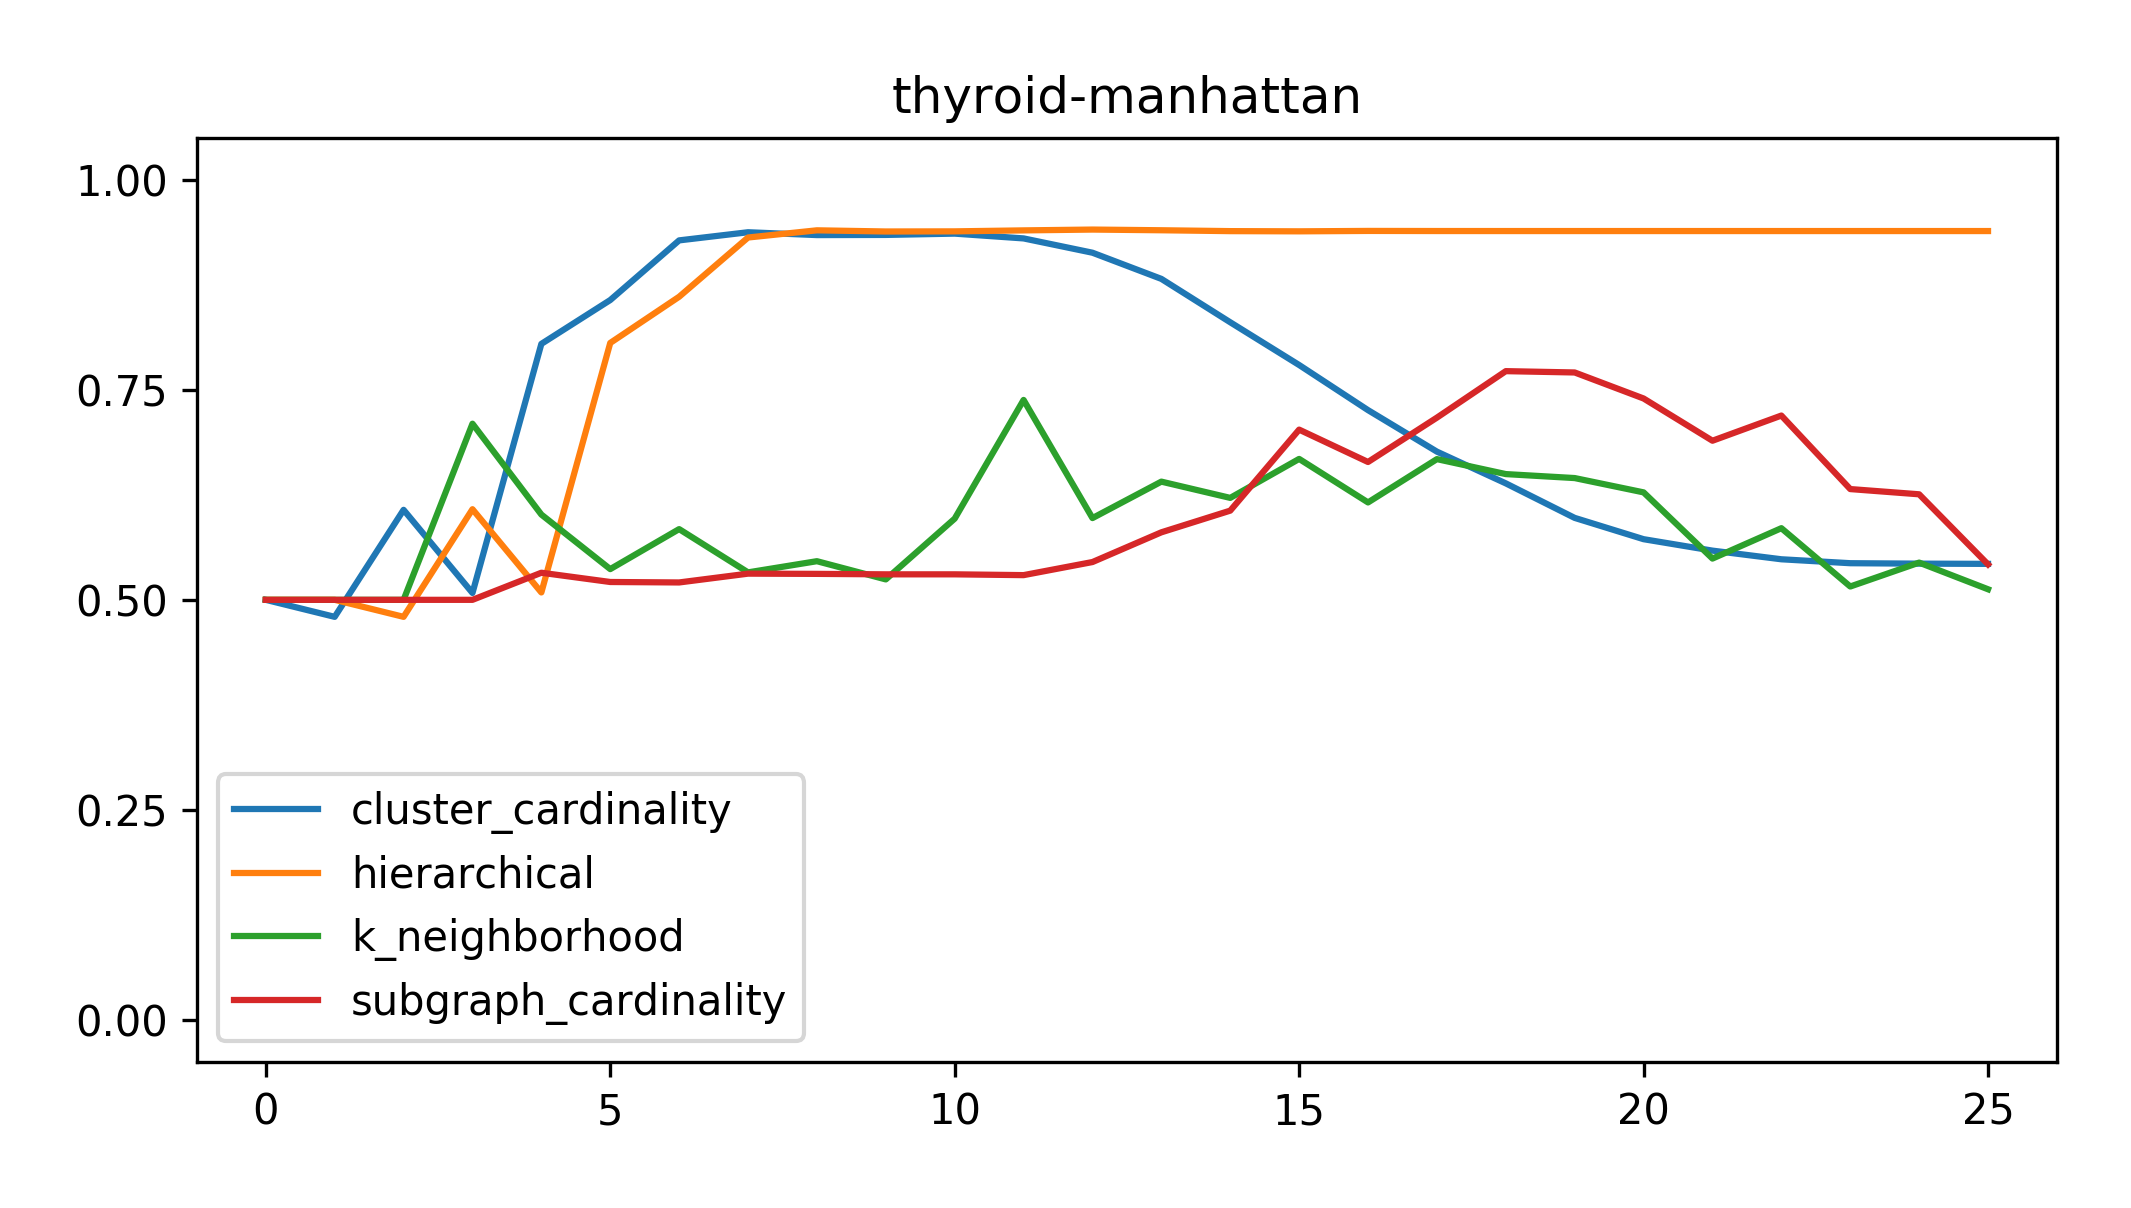
\includegraphics[width=2.2in]{kdd/static/auc_vs_depth/thyroid-manhattan.png}

% Vertebral
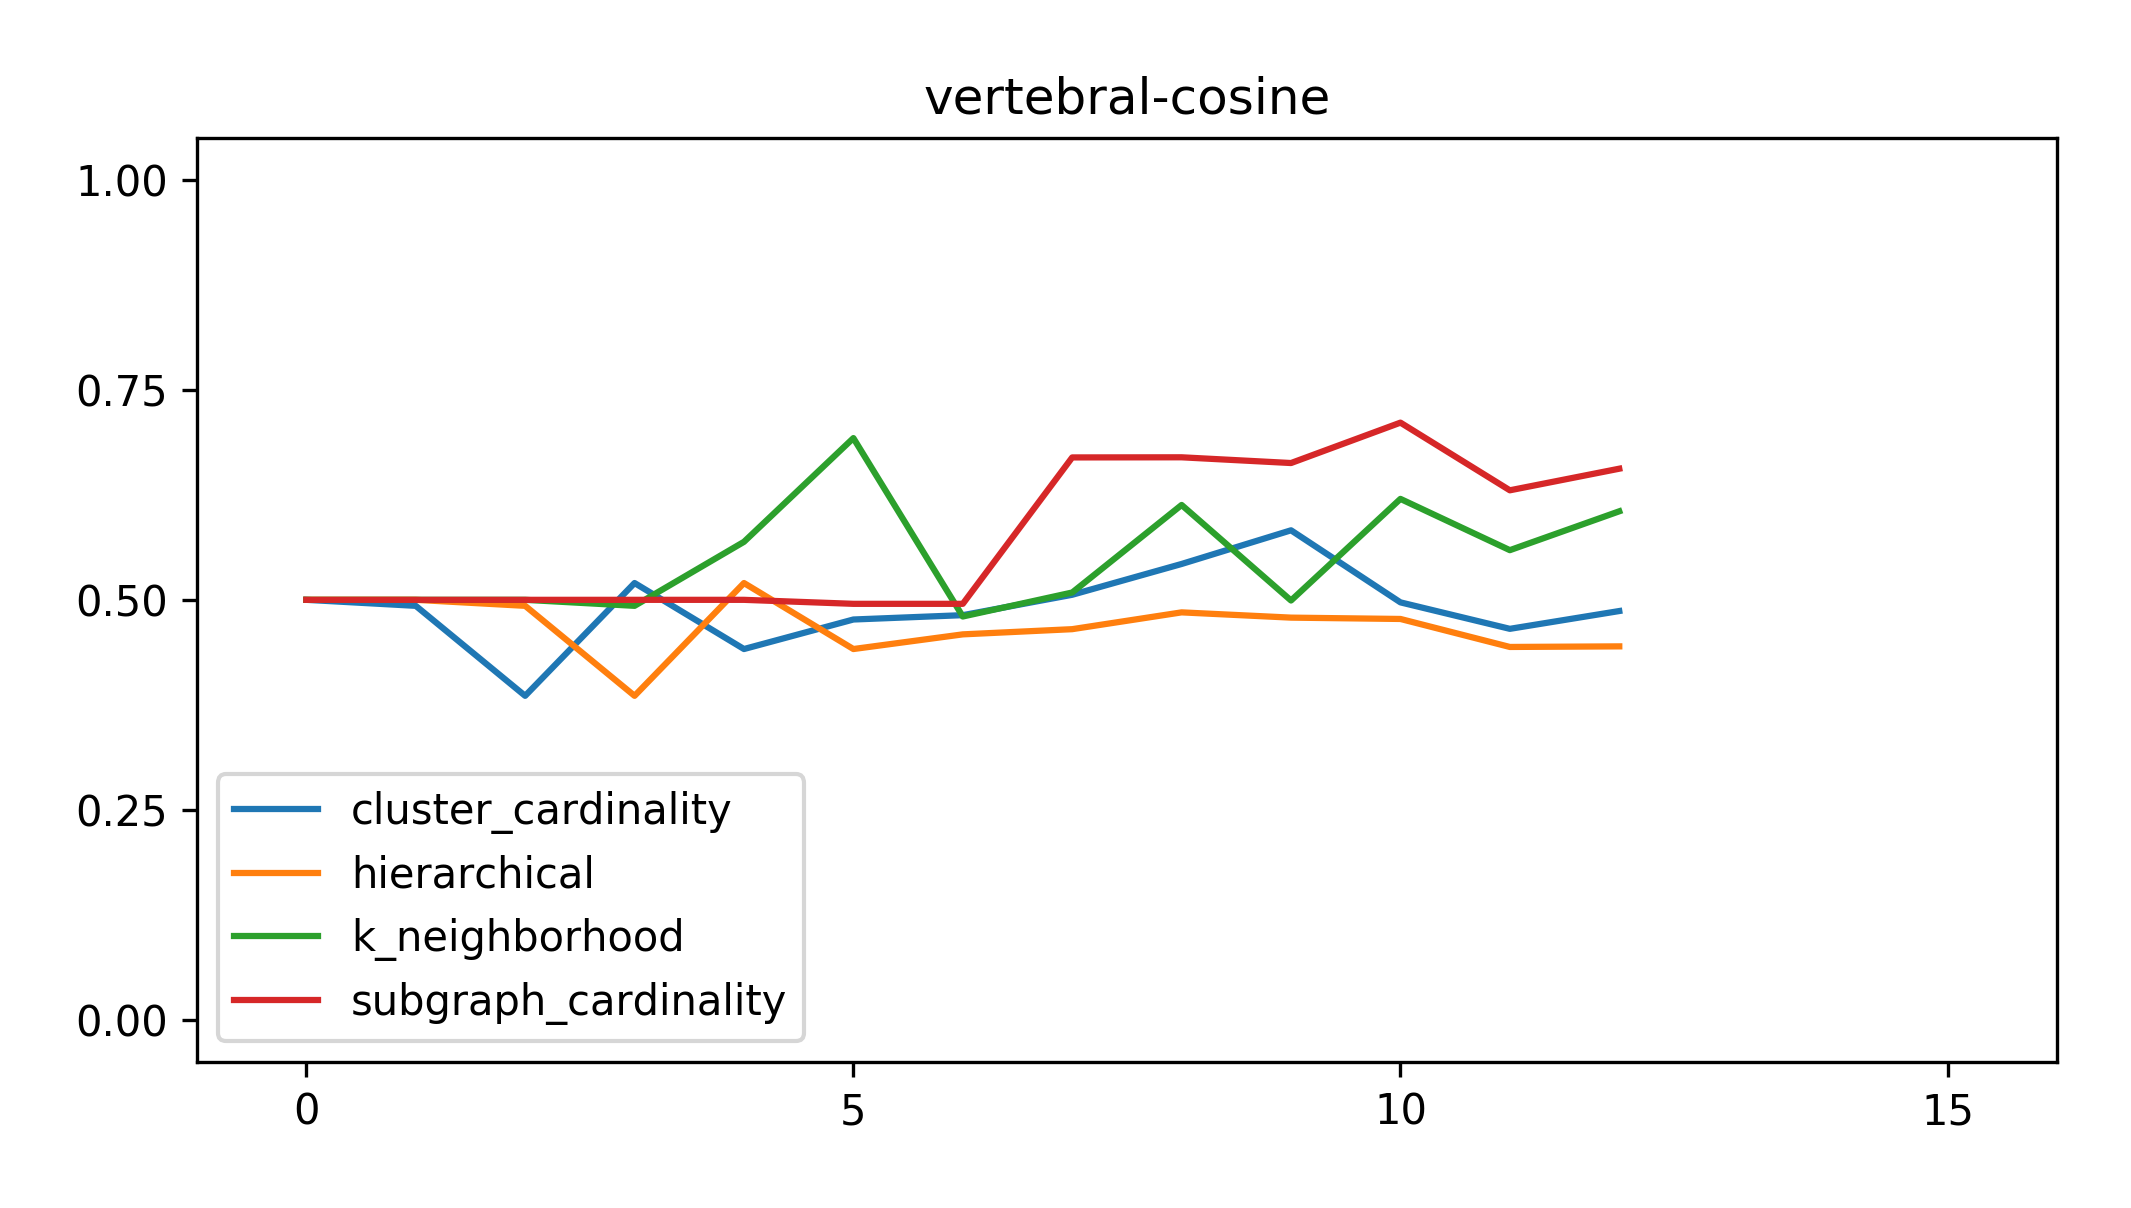
\includegraphics[width=2.2in]{kdd/static/auc_vs_depth/vertebral-cosine.png}
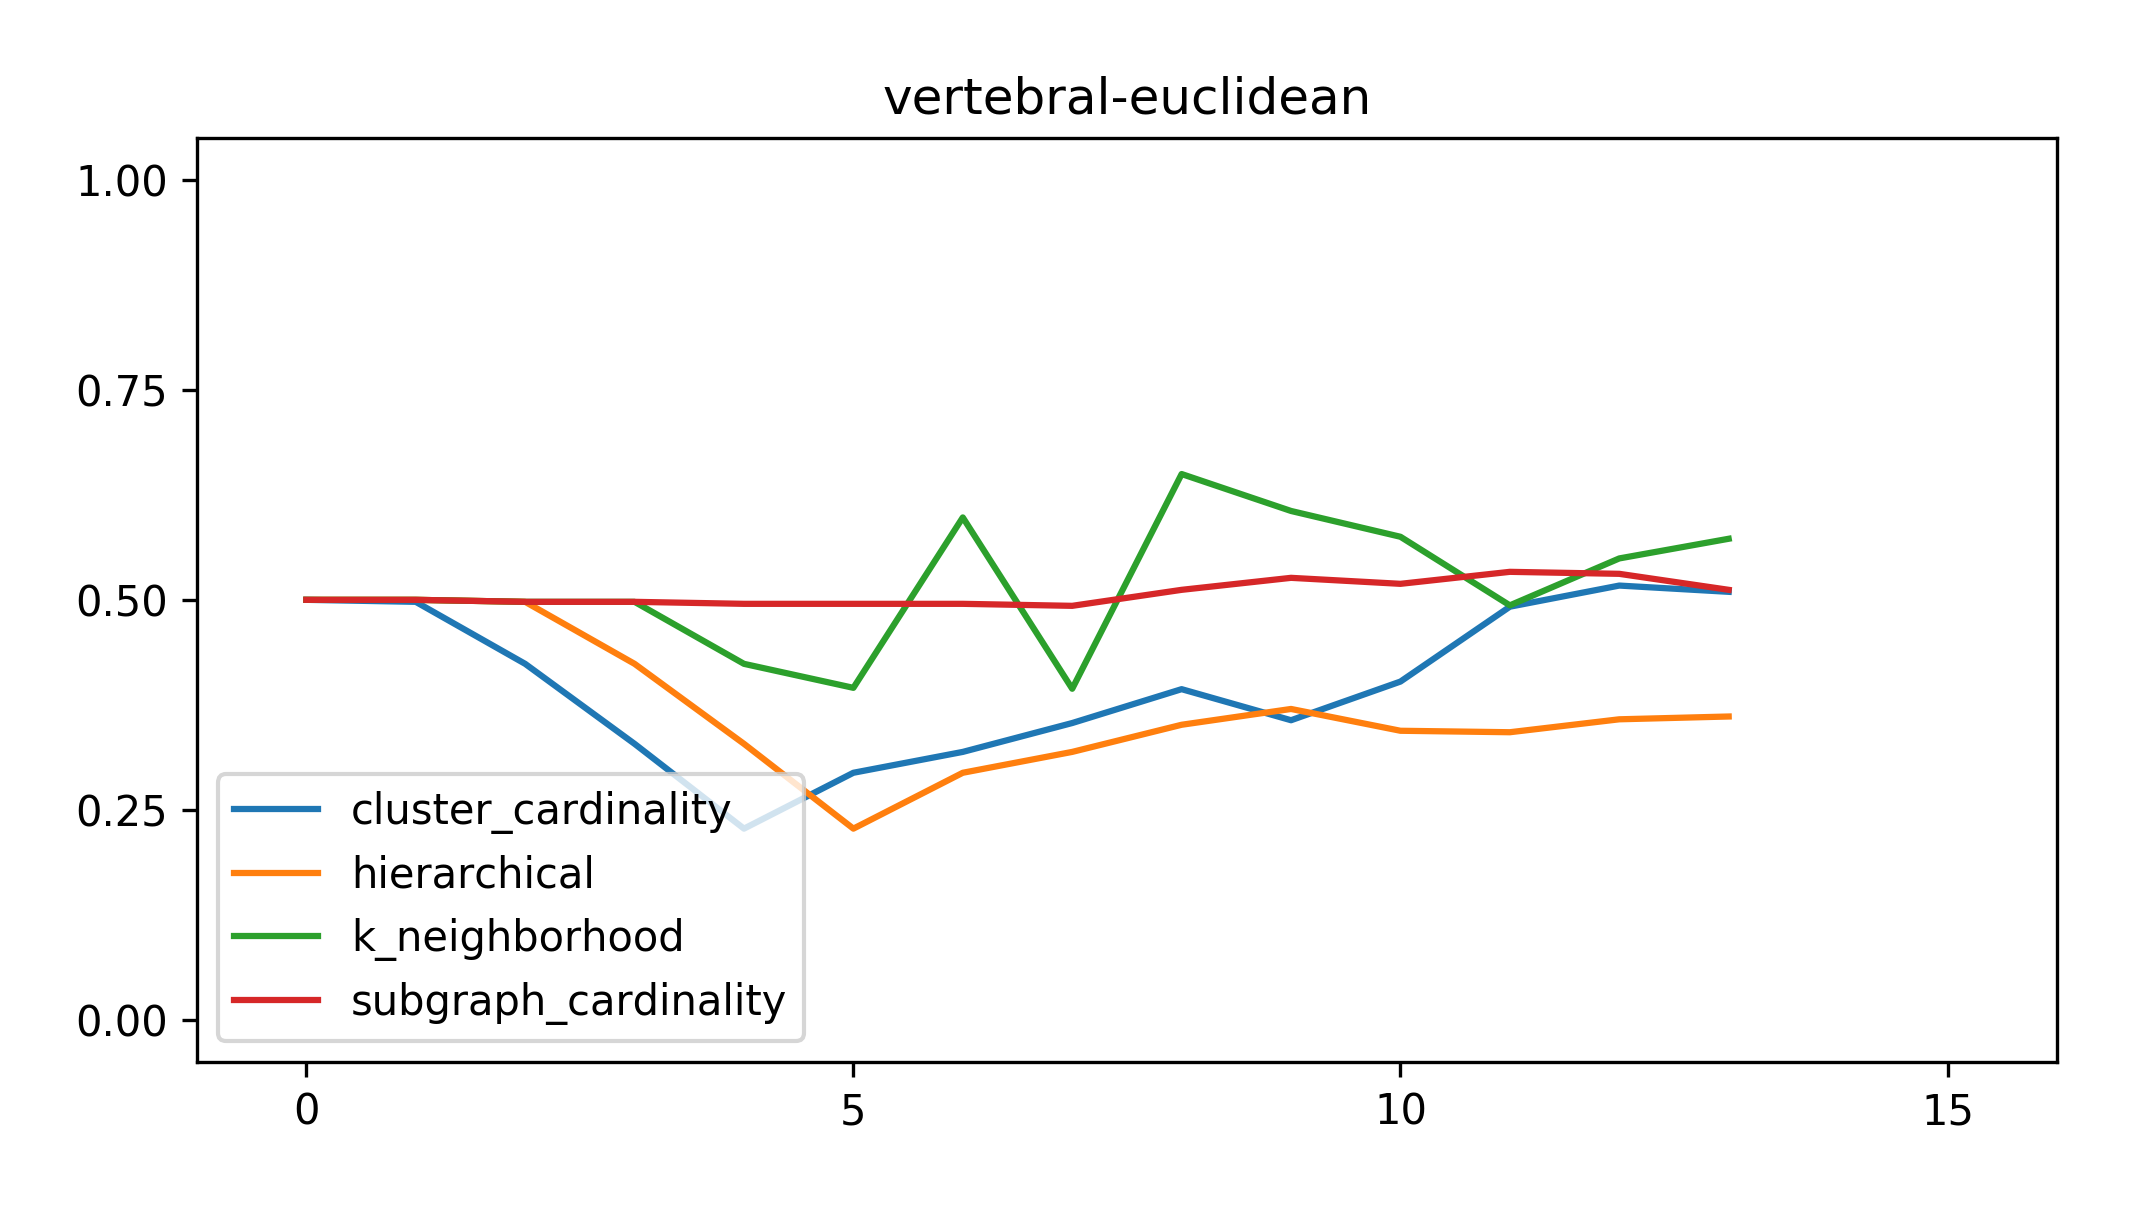
\includegraphics[width=2.2in]{kdd/static/auc_vs_depth/vertebral-euclidean.png}
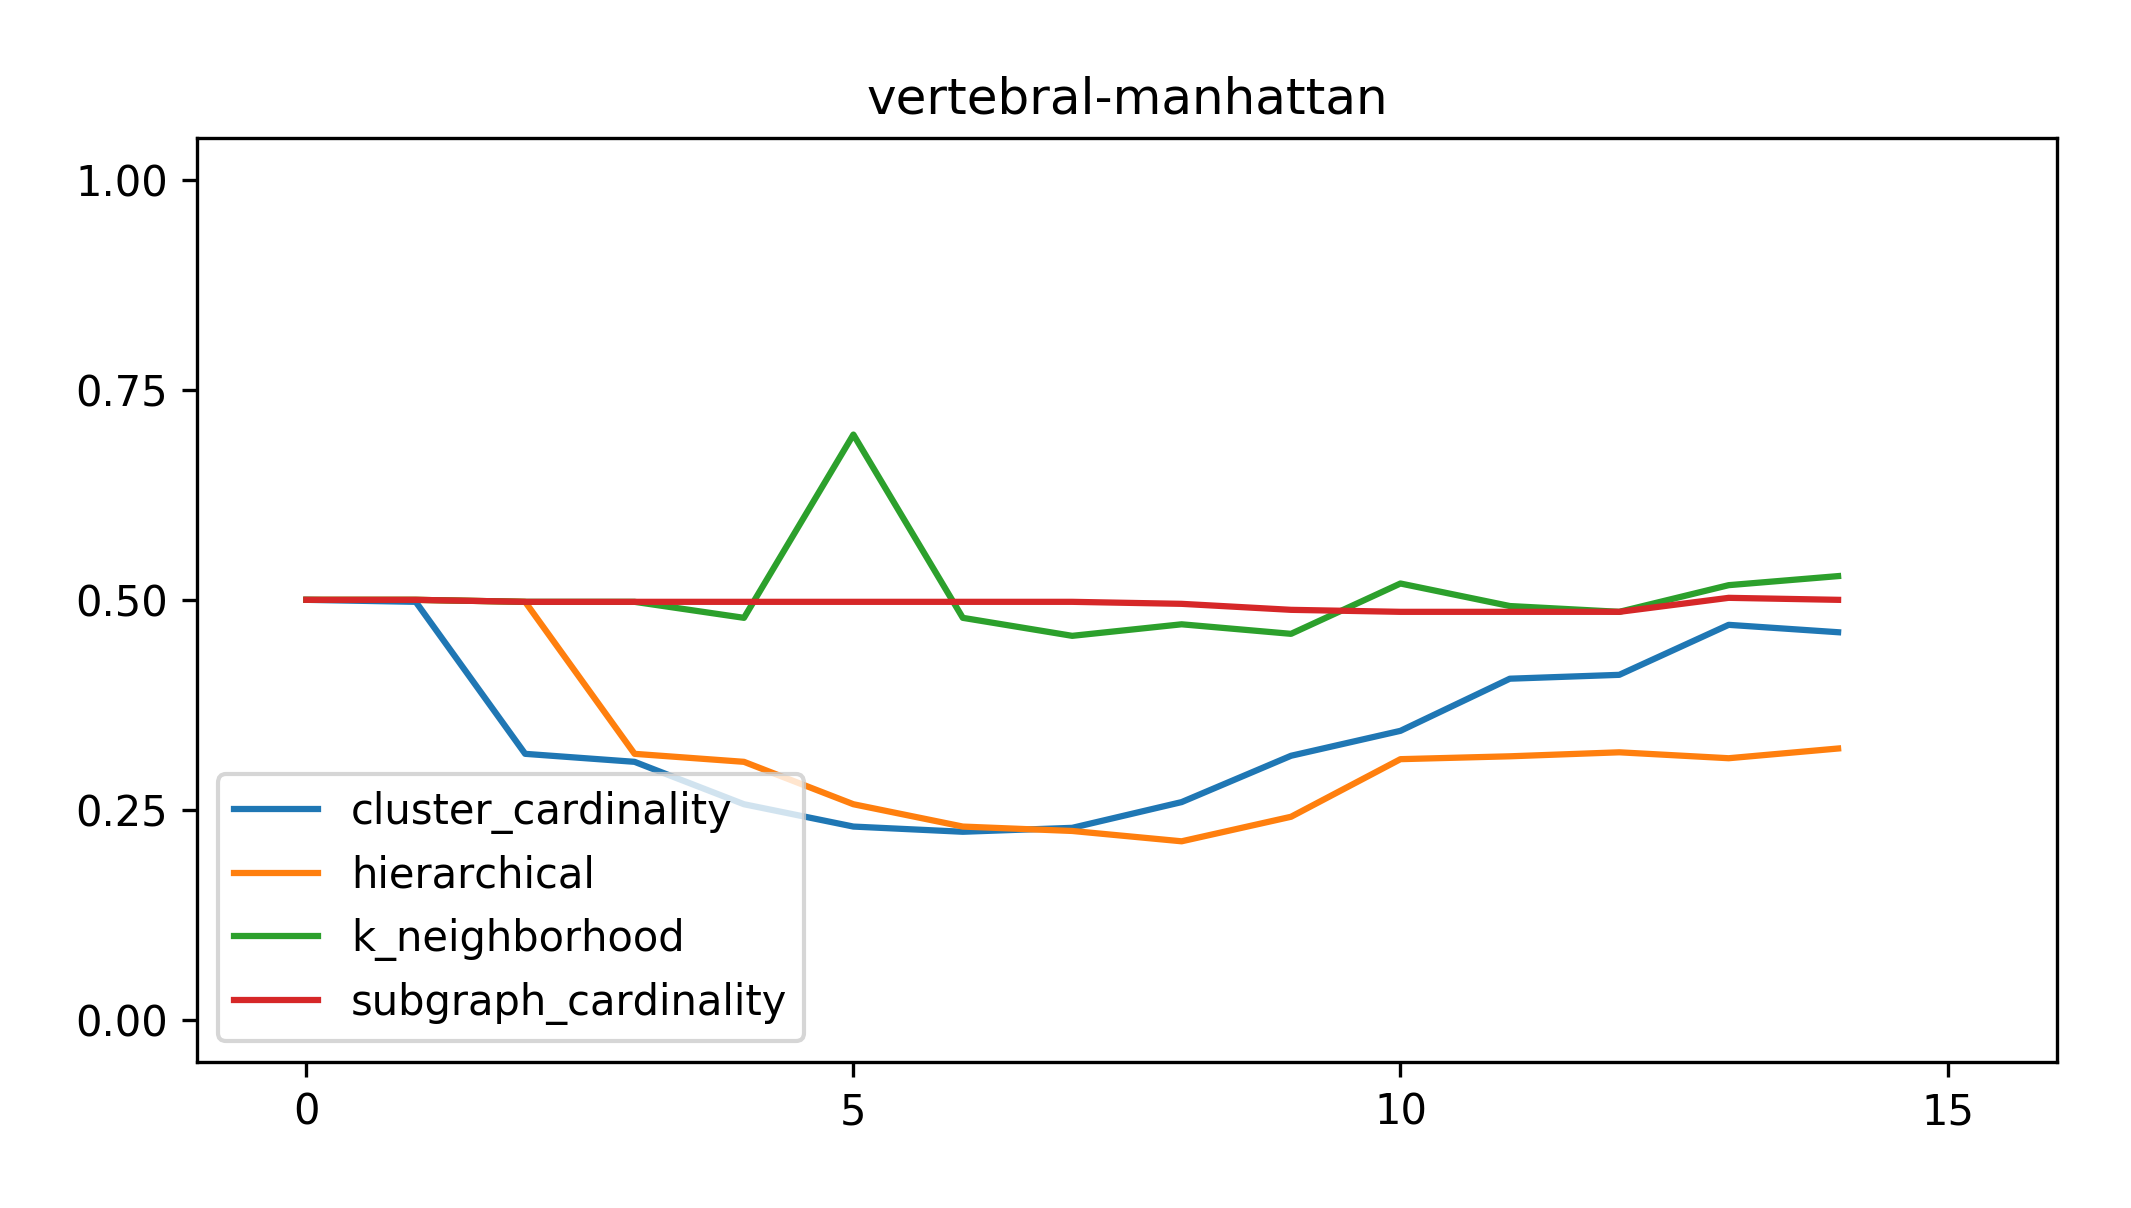
\includegraphics[width=2.2in]{kdd/static/auc_vs_depth/vertebral-manhattan.png}

% Vowels
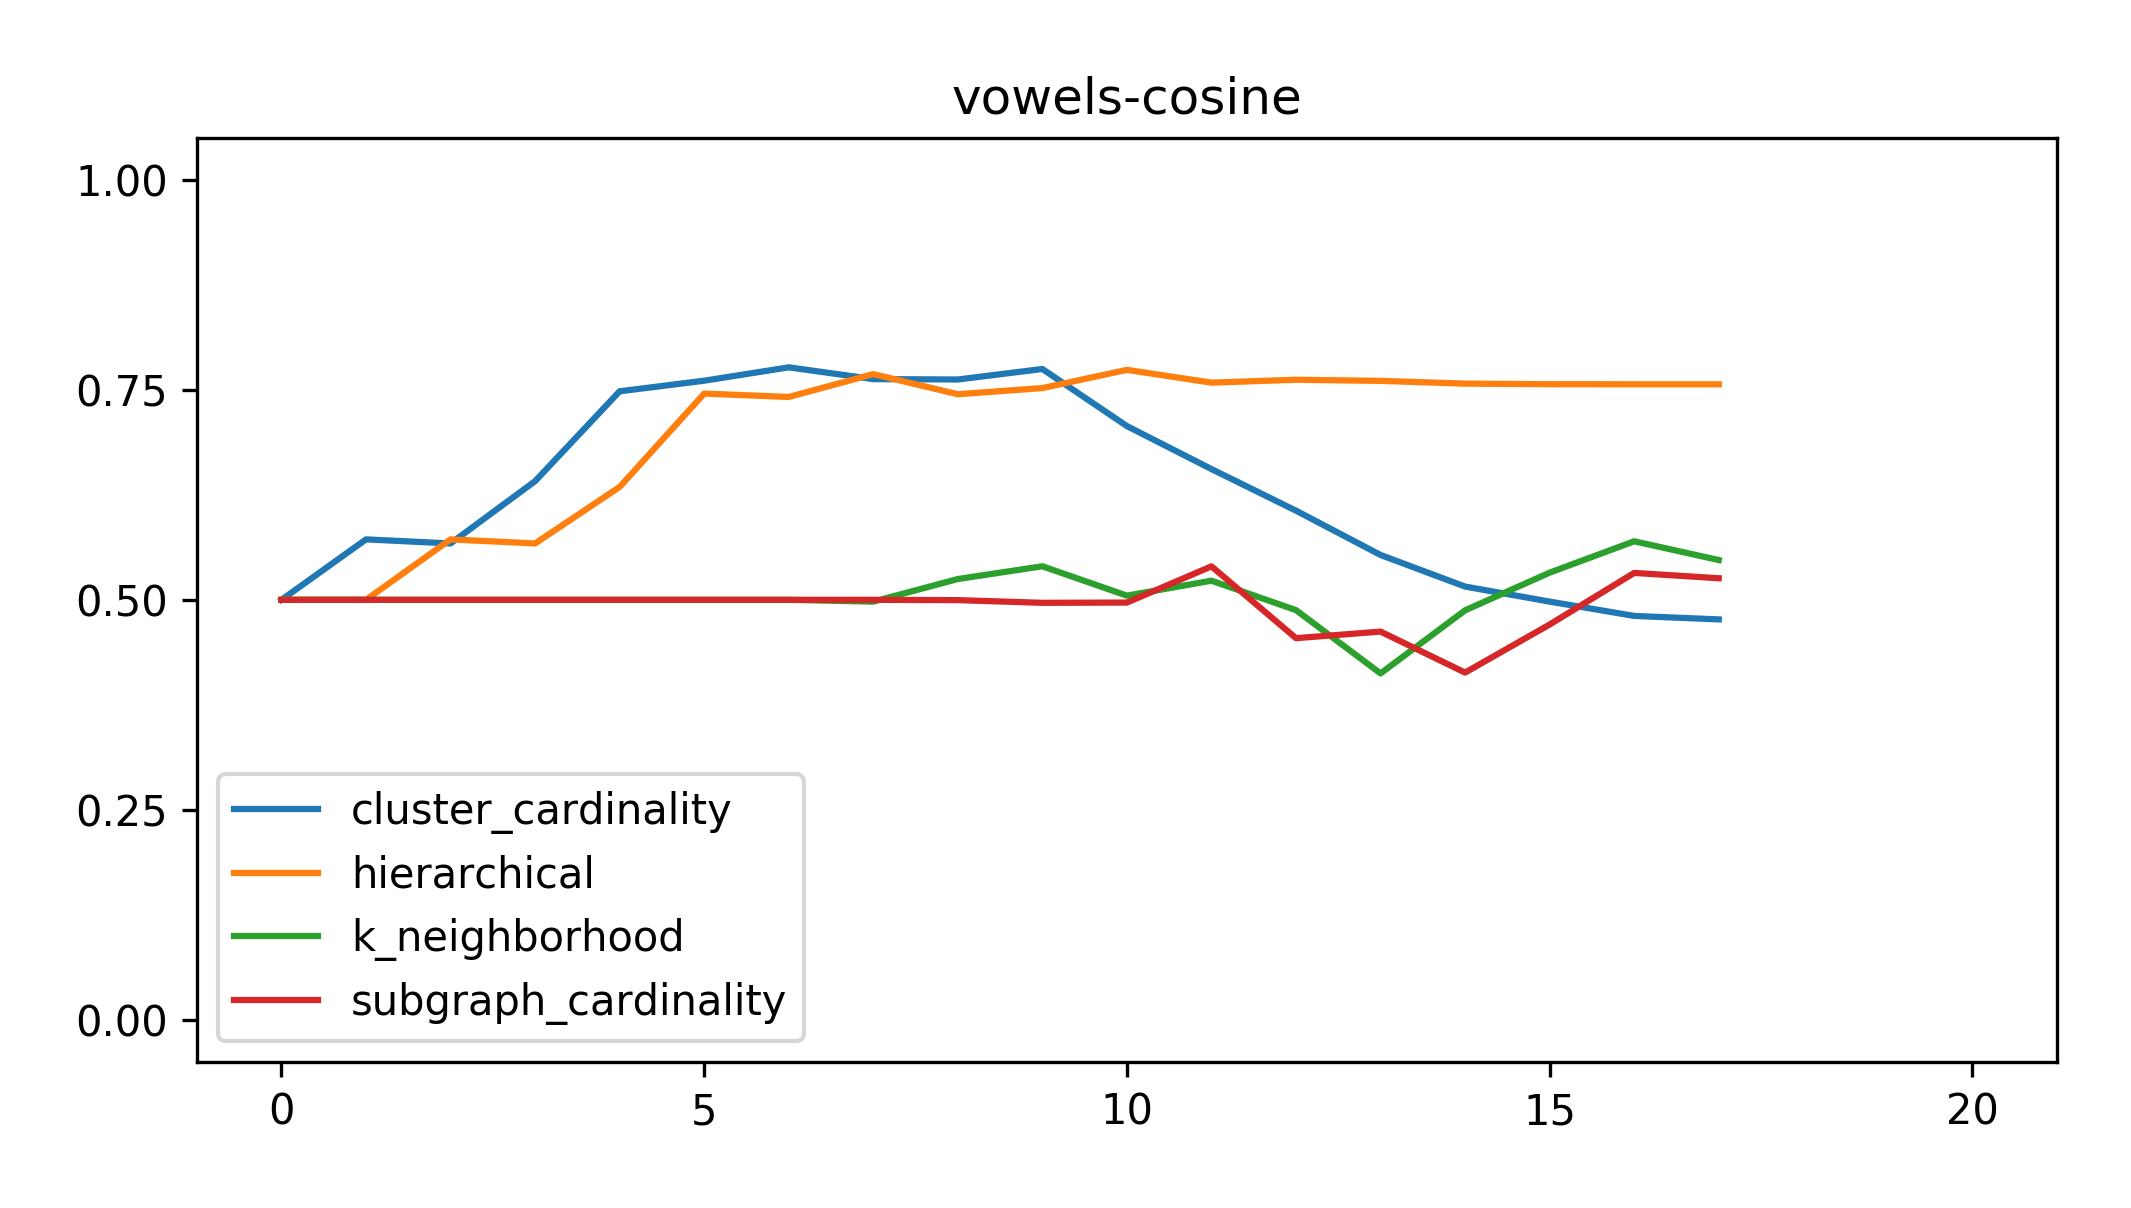
\includegraphics[width=2.2in]{kdd/static/auc_vs_depth/vowels-cosine.png}
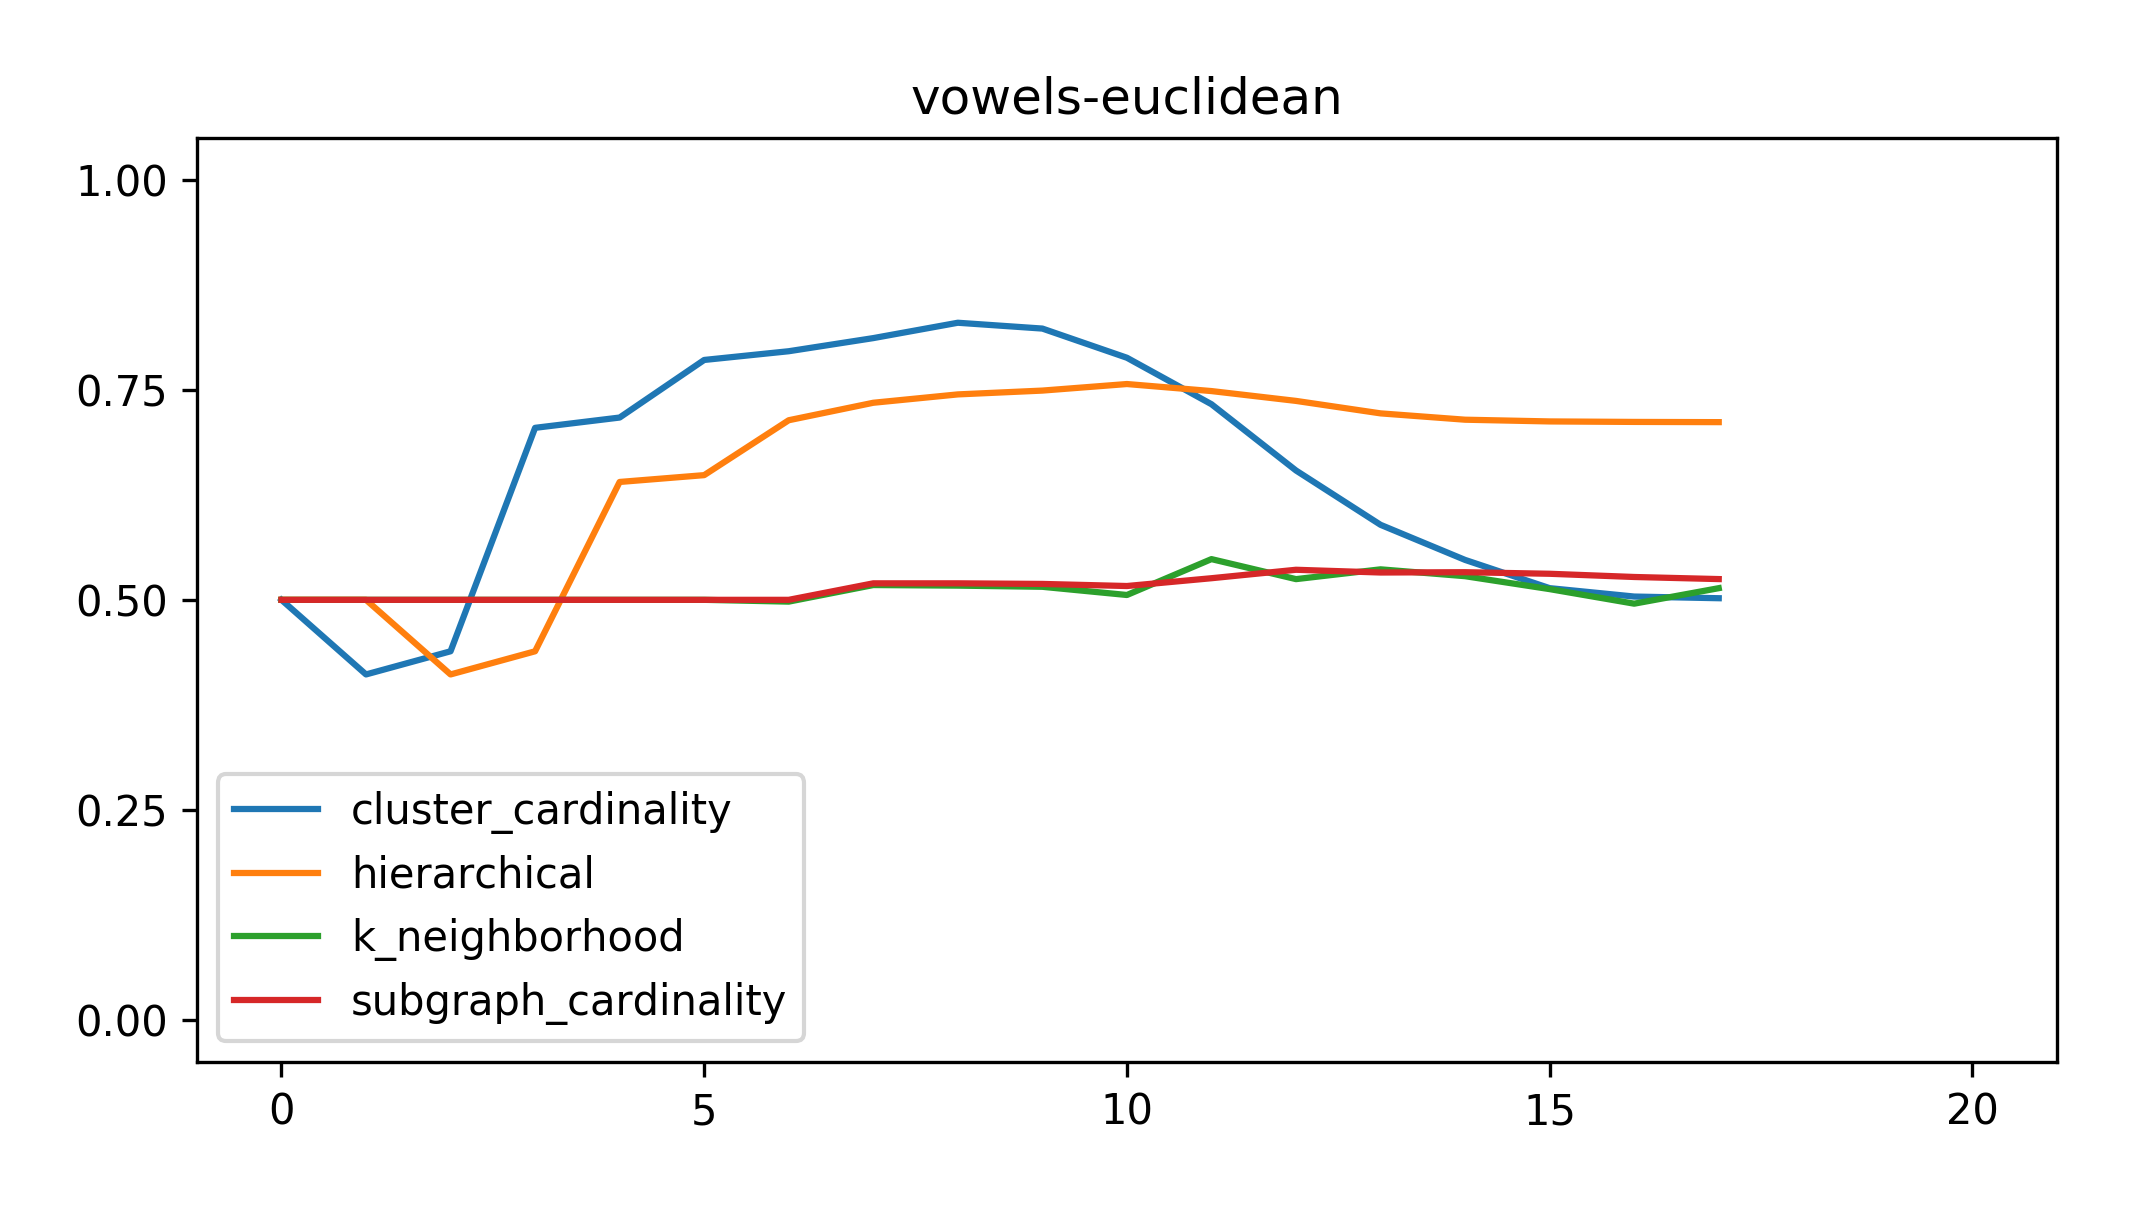
\includegraphics[width=2.2in]{kdd/static/auc_vs_depth/vowels-euclidean.png}
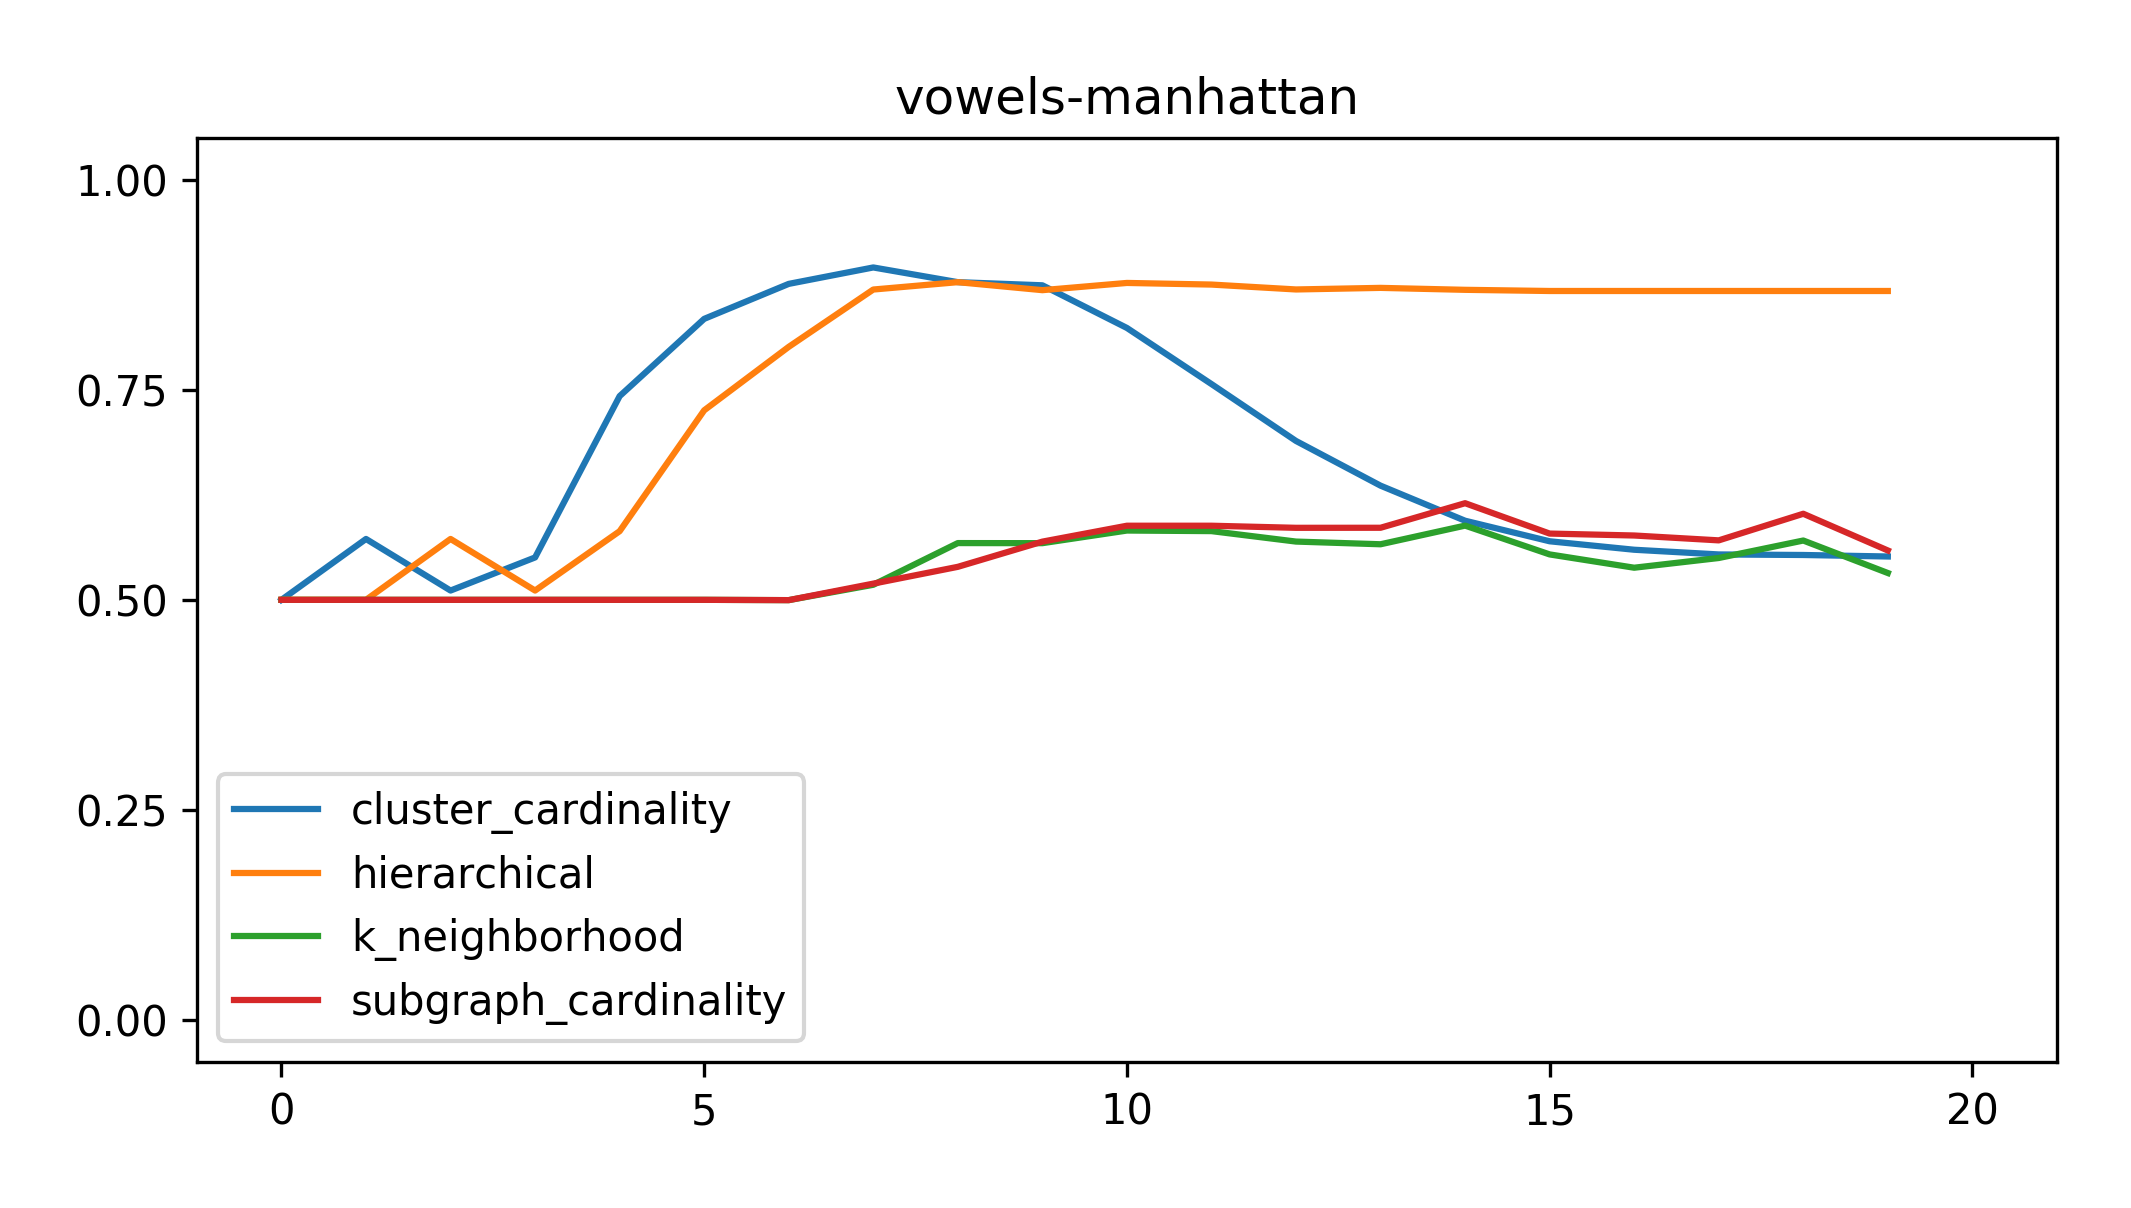
\includegraphics[width=2.2in]{kdd/static/auc_vs_depth/vowels-manhattan.png}

% WBC
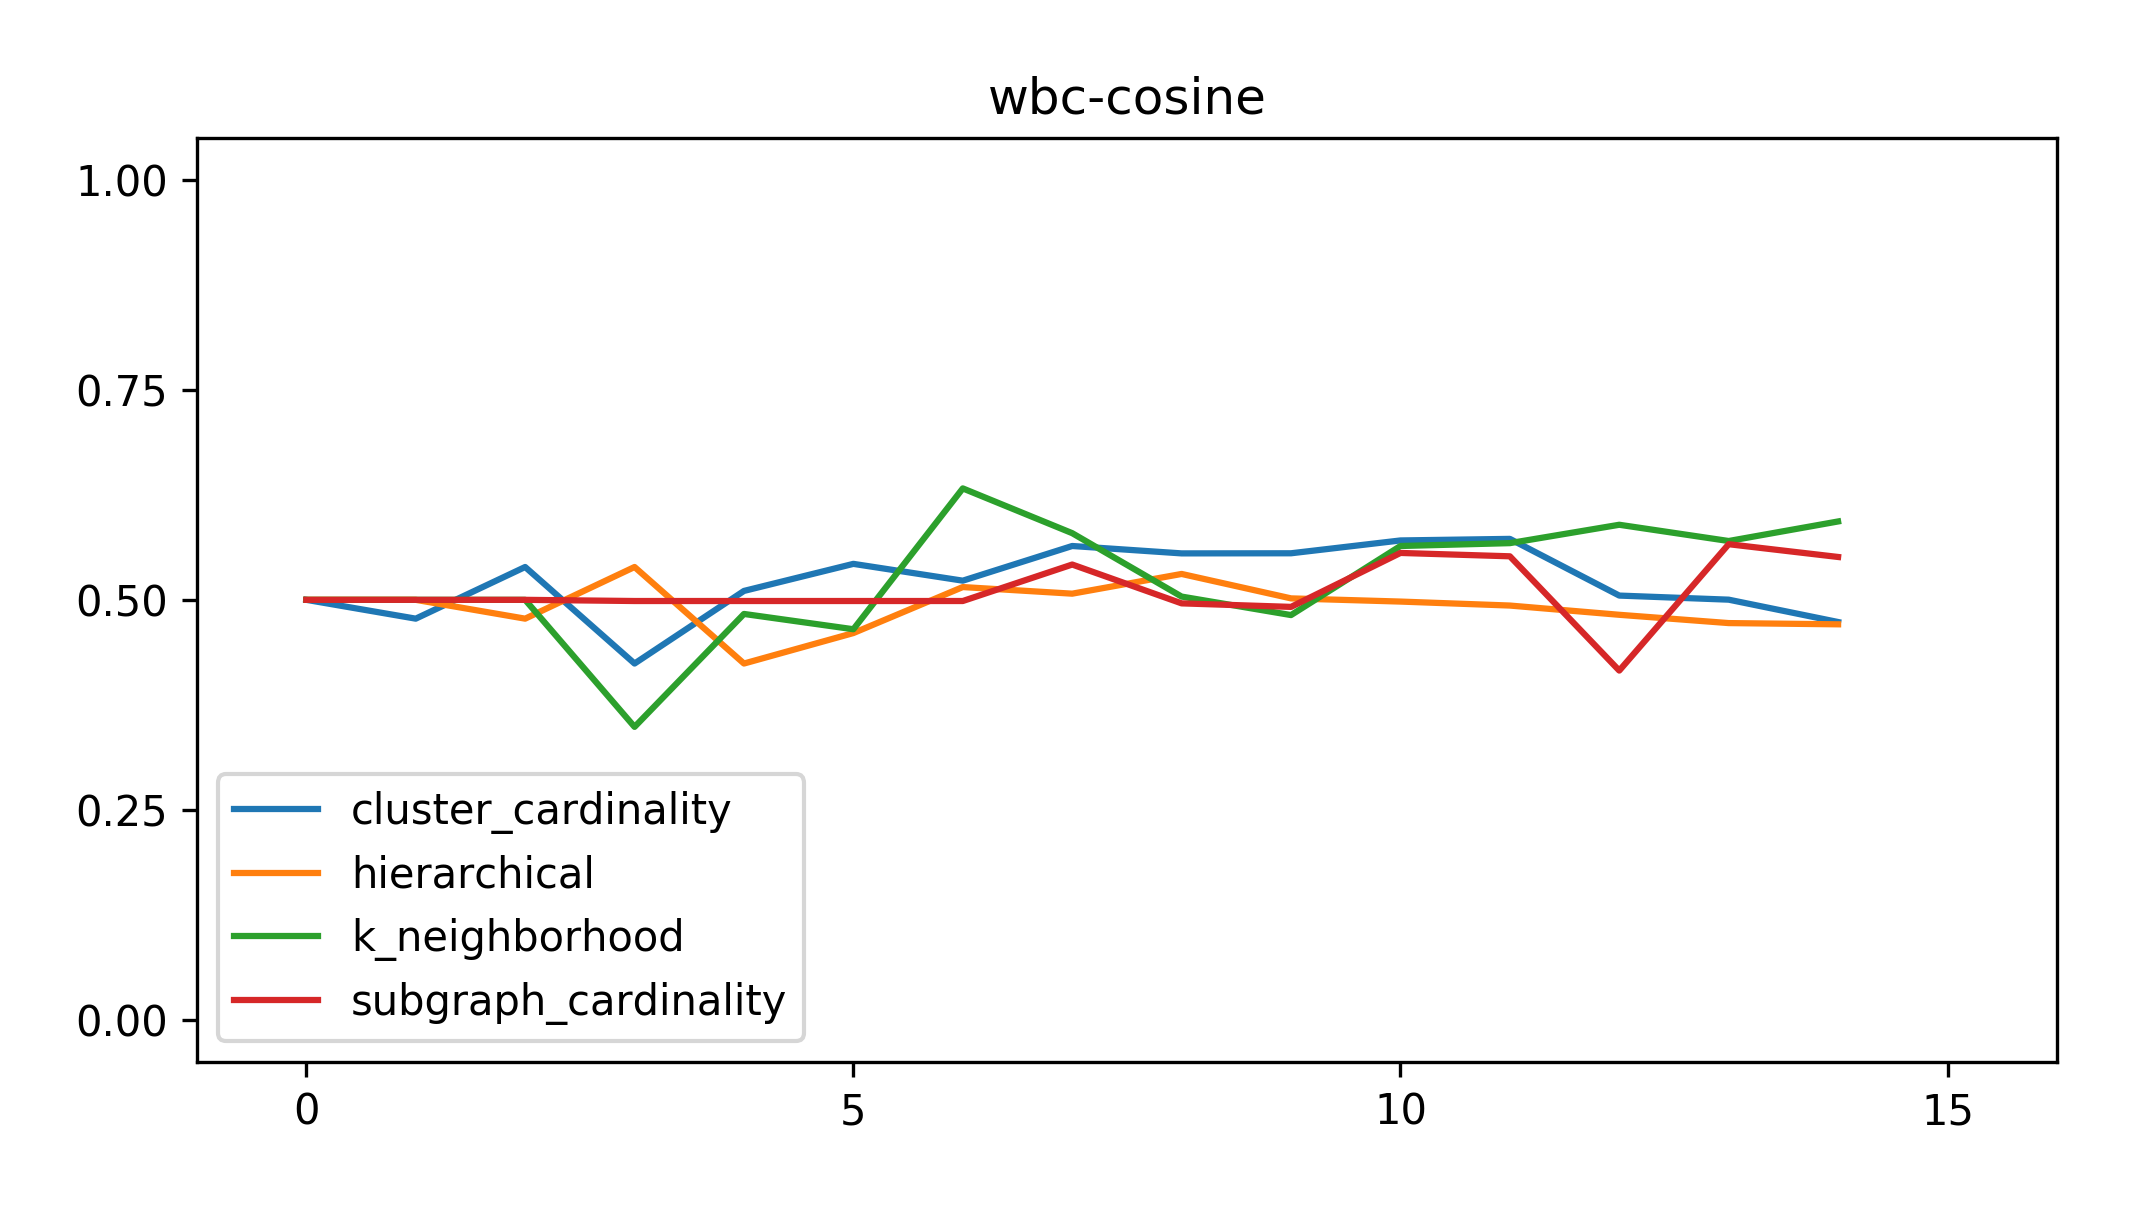
\includegraphics[width=2.2in]{kdd/static/auc_vs_depth/wbc-cosine.png}
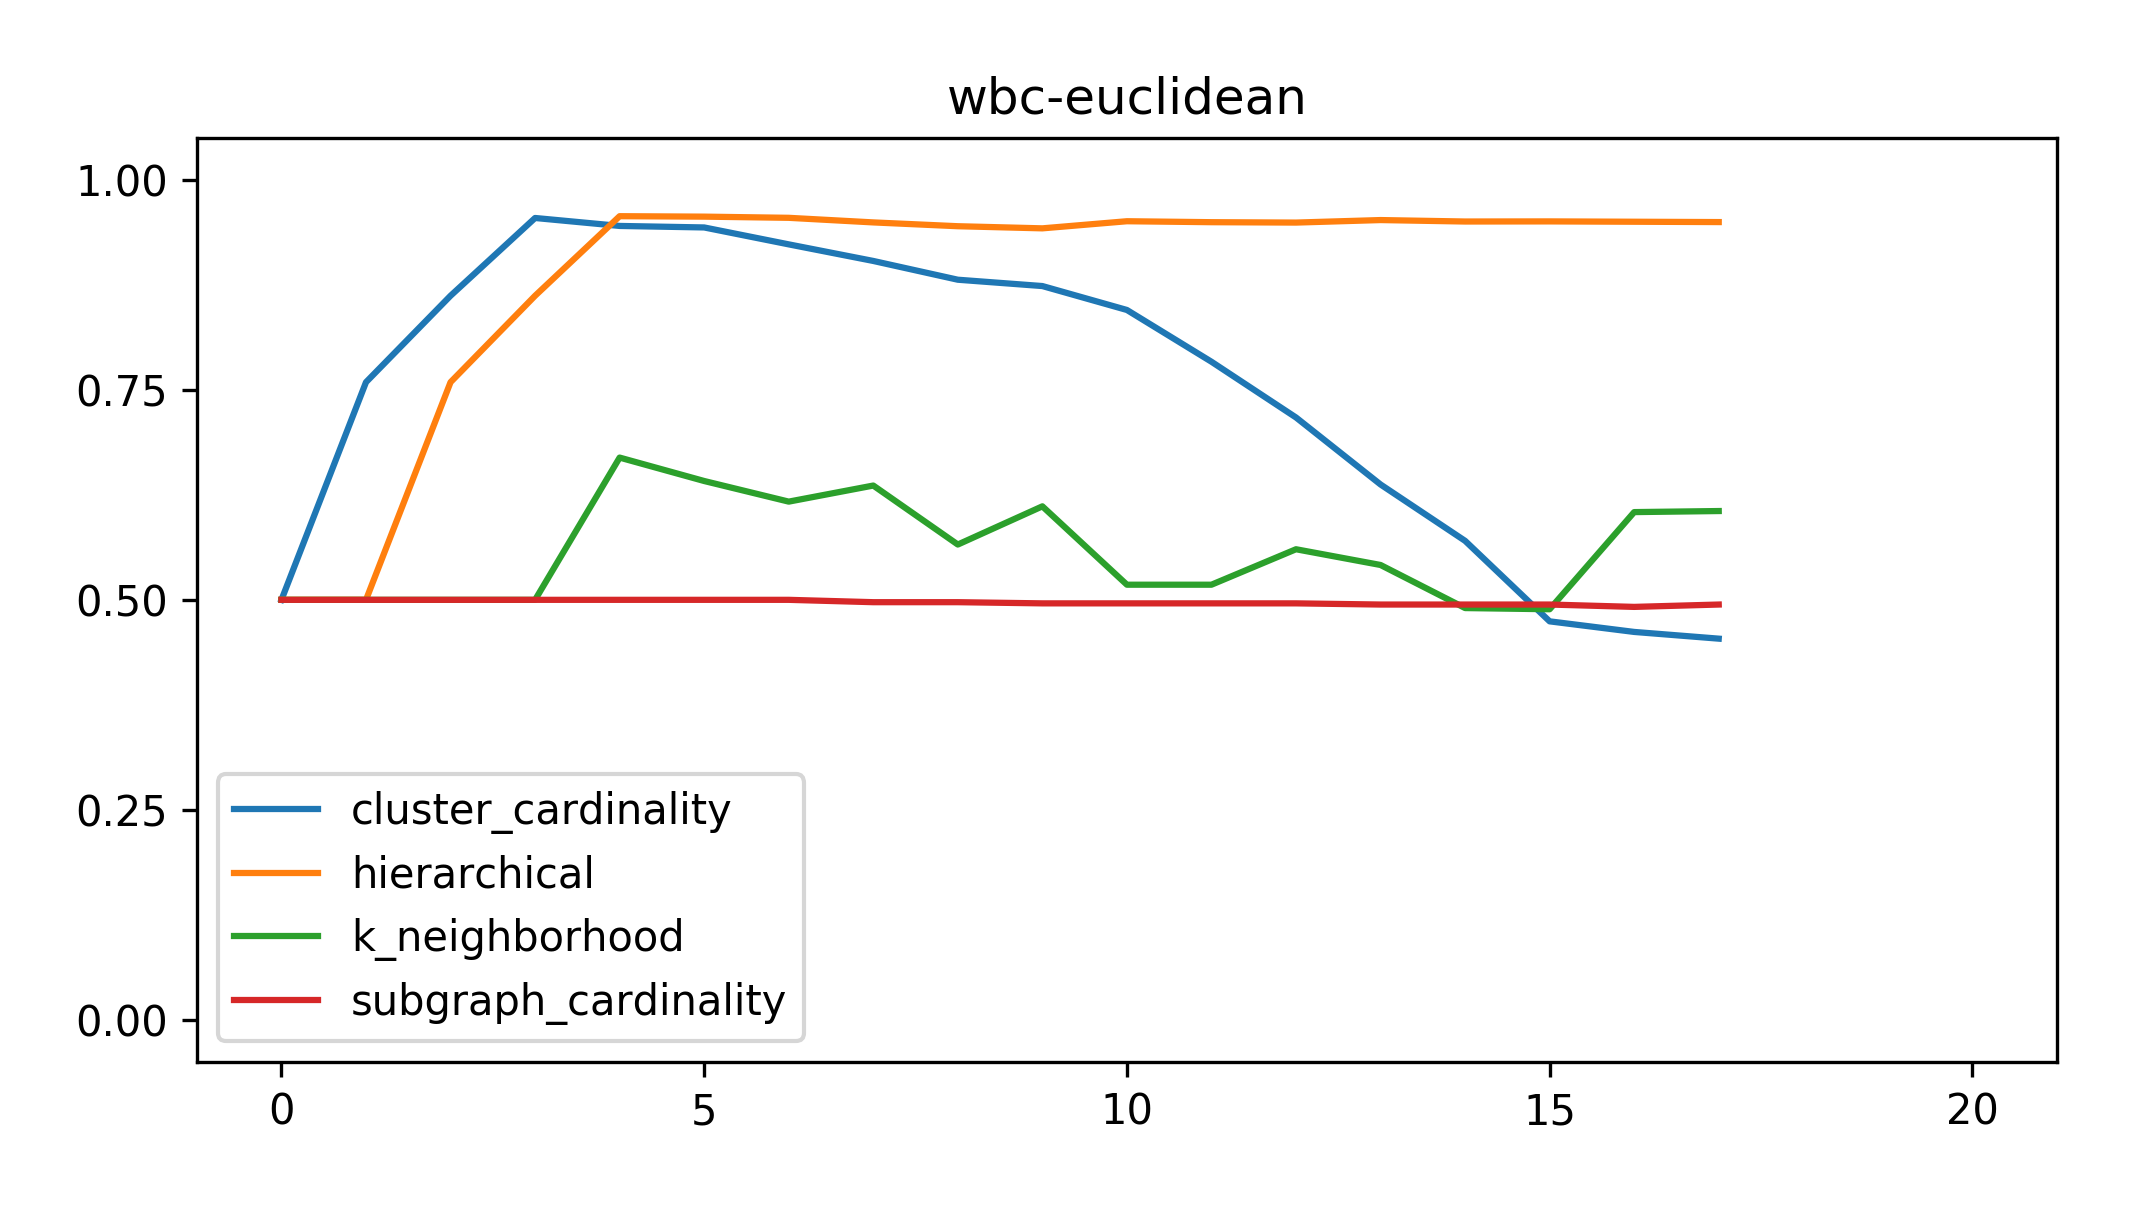
\includegraphics[width=2.2in]{kdd/static/auc_vs_depth/wbc-euclidean.png}
\includegraphics[width=2.2in]{kdd/static/auc_vs_depth/wbc-manhattan.png}

% Wine
\includegraphics[width=2.2in]{kdd/static/auc_vs_depth/wine-cosine.png}
\includegraphics[width=2.2in]{kdd/static/auc_vs_depth/wine-euclidean.png}
\includegraphics[width=2.2in]{kdd/static/auc_vs_depth/wine-manhattan.png}

\caption{
Plots of ROC-AUC vs Depth for our measures of Anomolousness.
}

\label{results:datasets_3}
\end{figure*}

\begin{figure*}[!t]
\centering

% HTTP
\includegraphics[width=2.2in]{kdd/static/auc_vs_depth/http-cosine.png}
\includegraphics[width=2.2in]{kdd/static/auc_vs_depth/http-euclidean.png}
\includegraphics[width=2.2in]{kdd/static/auc_vs_depth/http-manhattan.png}

% Shuttle
\includegraphics[width=2.2in]{kdd/static/auc_vs_depth/shuttle-cosine.png}
\includegraphics[width=2.2in]{kdd/static/auc_vs_depth/shuttle-euclidean.png}
\includegraphics[width=2.2in]{kdd/static/auc_vs_depth/shuttle-manhattan.png}

% SMTP
\includegraphics[width=2.2in]{kdd/static/auc_vs_depth/smtp-cosine.png}
\includegraphics[width=2.2in]{kdd/static/auc_vs_depth/smtp-euclidean.png}
\includegraphics[width=2.2in]{kdd/static/auc_vs_depth/smtp-manhattan.png}

% Pendigits
\includegraphics[width=2.2in]{kdd/static/auc_vs_depth/pendigits-cosine.png}
\includegraphics[width=2.2in]{kdd/static/auc_vs_depth/pendigits-euclidean.png}
\includegraphics[width=2.2in]{kdd/static/auc_vs_depth/pendigits-manhattan.png}

% Mammography
\includegraphics[width=2.2in]{kdd/static/auc_vs_depth/mammography-cosine.png}
\includegraphics[width=2.2in]{kdd/static/auc_vs_depth/mammography-euclidean.png}
\includegraphics[width=2.2in]{kdd/static/auc_vs_depth/mammography-manhattan.png}

\caption{
Plots of ROC-AUC vs Depth for our measures of Anomolousness.
}

\label{results:datasets_4}
\end{figure*}






\begin{figure*}[!t]
\centering
% Annthyroid
\includegraphics[width=2.2in]{kdd/static/lfd_vs_depth/annthyroid-cosine.png}
\includegraphics[width=2.2in]{kdd/static/lfd_vs_depth/annthyroid-euclidean.png}
\includegraphics[width=2.2in]{kdd/static/lfd_vs_depth/annthyroid-manhattan.png}

% Arrhythmia
\includegraphics[width=2.2in]{kdd/static/lfd_vs_depth/arrhythmia-cosine.png}
\includegraphics[width=2.2in]{kdd/static/lfd_vs_depth/arrhythmia-euclidean.png}
\includegraphics[width=2.2in]{kdd/static/lfd_vs_depth/arrhythmia-manhattan.png}

% BreastW
\includegraphics[width=2.2in]{kdd/static/lfd_vs_depth/breastw-cosine.png}
\includegraphics[width=2.2in]{kdd/static/lfd_vs_depth/breastw-euclidean.png}
\includegraphics[width=2.2in]{kdd/static/lfd_vs_depth/breastw-manhattan.png}

% Cardio
\includegraphics[width=2.2in]{kdd/static/lfd_vs_depth/cardio-cosine.png}
\includegraphics[width=2.2in]{kdd/static/lfd_vs_depth/cardio-euclidean.png}
\includegraphics[width=2.2in]{kdd/static/lfd_vs_depth/cardio-manhattan.png}

% Glass
\includegraphics[width=2.2in]{kdd/static/lfd_vs_depth/glass-cosine.png}
\includegraphics[width=2.2in]{kdd/static/lfd_vs_depth/glass-euclidean.png}
\includegraphics[width=2.2in]{kdd/static/lfd_vs_depth/glass-manhattan.png}

% Ionosphere
\includegraphics[width=2.2in]{kdd/static/auc_vs_depth/ionosphere-cosine.png}
\includegraphics[width=2.2in]{kdd/static/auc_vs_depth/ionosphere-euclidean.png}
\includegraphics[width=2.2in]{kdd/static/auc_vs_depth/ionosphere-manhattan.png}

\caption{
Plots of Local Fractal Dimension vs Depth for our datasets.
}

\label{results:lfd_1}
\end{figure*}

\begin{figure*}[!t]
\centering
% Lympho
\includegraphics[width=2.2in]{kdd/static/lfd_vs_depth/lympho-cosine.png}
\includegraphics[width=2.2in]{kdd/static/lfd_vs_depth/lympho-euclidean.png}
\includegraphics[width=2.2in]{kdd/static/lfd_vs_depth/lympho-manhattan.png}

% Mnist
\includegraphics[width=2.2in]{kdd/static/lfd_vs_depth/mnist-cosine.png}
\includegraphics[width=2.2in]{kdd/static/lfd_vs_depth/mnist-euclidean.png}
\includegraphics[width=2.2in]{kdd/static/lfd_vs_depth/mnist-manhattan.png}

% Musk
\includegraphics[width=2.2in]{kdd/static/lfd_vs_depth/musk-cosine.png}
\includegraphics[width=2.2in]{kdd/static/lfd_vs_depth/musk-euclidean.png}
\includegraphics[width=2.2in]{kdd/static/lfd_vs_depth/musk-manhattan.png}

% Optdigits
\includegraphics[width=2.2in]{kdd/static/lfd_vs_depth/optdigits-cosine.png}
\includegraphics[width=2.2in]{kdd/static/lfd_vs_depth/optdigits-euclidean.png}
\includegraphics[width=2.2in]{kdd/static/lfd_vs_depth/optdigits-manhattan.png}

% Pima
\includegraphics[width=2.2in]{kdd/static/lfd_vs_depth/pima-cosine.png}
\includegraphics[width=2.2in]{kdd/static/lfd_vs_depth/pima-euclidean.png}
\includegraphics[width=2.2in]{kdd/static/lfd_vs_depth/pima-manhattan.png}

% Satellite
\includegraphics[width=2.2in]{kdd/static/lfd_vs_depth/satellite-cosine.png}
\includegraphics[width=2.2in]{kdd/static/lfd_vs_depth/satellite-euclidean.png}
\includegraphics[width=2.2in]{kdd/static/lfd_vs_depth/satellite-manhattan.png}

\caption{
Plots of Local Fractal Dimension vs Depth for our datasets.
}

\label{results:lfd_2}
\end{figure*}

\begin{figure*}[!t]
\centering
% Satimage-2
\includegraphics[width=2.2in]{kdd/static/lfd_vs_depth/satimage-2-cosine.png}
\includegraphics[width=2.2in]{kdd/static/lfd_vs_depth/satimage-2-euclidean.png}
\includegraphics[width=2.2in]{kdd/static/lfd_vs_depth/satimage-2-manhattan.png}

% Thyroid
\includegraphics[width=2.2in]{kdd/static/lfd_vs_depth/thyroid-cosine.png}
\includegraphics[width=2.2in]{kdd/static/lfd_vs_depth/thyroid-euclidean.png}
\includegraphics[width=2.2in]{kdd/static/lfd_vs_depth/thyroid-manhattan.png}

% Vertebral
\includegraphics[width=2.2in]{kdd/static/lfd_vs_depth/vertebral-cosine.png}
\includegraphics[width=2.2in]{kdd/static/lfd_vs_depth/vertebral-euclidean.png}
\includegraphics[width=2.2in]{kdd/static/lfd_vs_depth/vertebral-manhattan.png}

% Vowels
\includegraphics[width=2.2in]{kdd/static/lfd_vs_depth/vowels-cosine.png}
\includegraphics[width=2.2in]{kdd/static/lfd_vs_depth/vowels-euclidean.png}
\includegraphics[width=2.2in]{kdd/static/lfd_vs_depth/vowels-manhattan.png}

% WBC
\includegraphics[width=2.2in]{kdd/static/lfd_vs_depth/wbc-cosine.png}
\includegraphics[width=2.2in]{kdd/static/lfd_vs_depth/wbc-euclidean.png}
\includegraphics[width=2.2in]{kdd/static/lfd_vs_depth/wbc-manhattan.png}

% Wine
\includegraphics[width=2.2in]{kdd/static/lfd_vs_depth/wine-cosine.png}
\includegraphics[width=2.2in]{kdd/static/lfd_vs_depth/wine-euclidean.png}
\includegraphics[width=2.2in]{kdd/static/lfd_vs_depth/wine-manhattan.png}

\caption{
Plots of Local Fractal Dimension vs Depth for our datasets.
}

\label{results:lfd_3}
\end{figure*}

\begin{figure*}[!t]
\centering

% HTTP
\includegraphics[width=2.2in]{kdd/static/lfd_vs_depth/http-cosine.png}
\includegraphics[width=2.2in]{kdd/static/lfd_vs_depth/http-euclidean.png}
\includegraphics[width=2.2in]{kdd/static/lfd_vs_depth/http-manhattan.png}

% Shuttle
\includegraphics[width=2.2in]{kdd/static/lfd_vs_depth/shuttle-cosine.png}
\includegraphics[width=2.2in]{kdd/static/lfd_vs_depth/shuttle-euclidean.png}
\includegraphics[width=2.2in]{kdd/static/lfd_vs_depth/shuttle-manhattan.png}

% SMTP
\includegraphics[width=2.2in]{kdd/static/lfd_vs_depth/smtp-cosine.png}
\includegraphics[width=2.2in]{kdd/static/lfd_vs_depth/smtp-euclidean.png}
\includegraphics[width=2.2in]{kdd/static/lfd_vs_depth/smtp-manhattan.png}

% Pendigits
\includegraphics[width=2.2in]{kdd/static/lfd_vs_depth/pendigits-cosine.png}
\includegraphics[width=2.2in]{kdd/static/lfd_vs_depth/pendigits-euclidean.png}
\includegraphics[width=2.2in]{kdd/static/lfd_vs_depth/pendigits-manhattan.png}

% Mammography
\includegraphics[width=2.2in]{kdd/static/lfd_vs_depth/mammography-cosine.png}
\includegraphics[width=2.2in]{kdd/static/lfd_vs_depth/mammography-euclidean.png}
\includegraphics[width=2.2in]{kdd/static/lfd_vs_depth/mammography-manhattan.png}

\caption{
Plots of Local Fractal Dimension vs Depth for our datasets.
}

\label{results:lfd_4}
\end{figure*}

